 %%%%%%%%%%%%%%%%%%%%%%%%%%%%%%%%%%%%%%%%%%%%%%%%%
%------ LaTeX-Dokument f�r die gesamte Bachelorarbeit --------
%%%%%%%%%%%%%%%%%%%%%%%%%%%%%%%%%%%%%%%%%%%%%%%%%


%---- Header (mit Formateinstellugen) laden, Inputencoding pr�fen ------
%%%%%%%%%%%%%%%%%%%%%%%%%%%%%%%%%%%%%%%%%%%%%%%%%
%---- LaTeX-Header fuer Abschlussarbeiten, Prof. Thomas Goerne, Dez. 2012/Aug. 2013 ----
%%%%%%%%%%%%%%%%%%%%%%%%%%%%%%%%%%%%%%%%%%%%%%%%%

\documentclass[12pt,paper=A4,parskip=half, pointlessnumbers,bibtotoc,liststotoc,DIV=11,BCOR=1mm]{scrreprt}
% BCOR ist die Bindekorrektur (verlorener Rand am linken Blattrand)! Wert haengt von der Art der Heftung ab!!
% DIV ist eine Satzspiegeleinstellung von KOMA-Script / sccreprt.

\pagestyle{headings}

\usepackage[T1]{fontenc} % Font Encoding fuer europaeische Schriften mit Umlauten (Unterstuetzung der Worttrennung)
\usepackage{lmodern} % PostScript-Varianten der TeX Computer Modern-Schriften laden
\usepackage[english,ngerman]{babel} % Spracheinstellungen fuer Englisch und Neudeutsch laden

\usepackage{graphicx} % Grafikeinbindung (fuer .JPG, .JPEG, .PNG und .PDF, falls pdflatex benutzt wird)
\usepackage[table]{xcolor} % ermoeglicht farbige Schrift und farbige Tabellenzeilen
\definecolor{black}{gray}{0} % Umdefinition der Farbe black, falls noetig (0=schwarz, 1=weiss)
\definecolor{dblue}{rgb}{0.1,0.2,0.6} % Dunkelblau, fuer Hyperlinks
\definecolor{lgray}{gray}{0.9} % Hellgrau, fuer Tabellen (0=schwarz, 1=weiss)

\usepackage{booktabs} % fuer schoene Tabellen

\usepackage[round,authoryear]{natbib} % Literaturverweise mit Name/Jahreszahl in runden Klammern
\bibpunct[:\,]{(}{)}{,}{a}{}{,~}  % Feinformatierung der Natbib-Zitierweise

\usepackage[hyphens]{url}
\usepackage[colorlinks=true,linkcolor=black,citecolor=dblue,urlcolor=dblue]{hyperref} 
\usepackage{hyperref}  
% die Pakete url und hyperref ermoeglichen anklickbare URLs im Quellenverzeichnis in definierter Farbe, 
% sie ermoeglichen den Zeilenumbruch bei langen URLs, und sie erzeugen Hyperlinks (Farbe s.o.) 
% zwischen Quellenverweis und Quellenverzeichnis sowie zwischen label und ref im PDF-Dokument

% Fonteinstellungen fuer Bildunterschriften: Unterschrift serifenlos, "Abbildung" fett (bfseries = bold face series)
\setkomafont{captionlabel}{\sffamily\bfseries}
\setkomafont{caption}{\sffamily}

%---- eigene Packages ------
%\usepackage[usenames,dvipsnames,svgnames,table]{xcolor}
\usepackage{acronym}
\usepackage[latin1]{inputenc} % Inputencoding f�r PC/Win
\usepackage{tikz}
\usepackage{amsmath, amssymb}
\usepackage{mathtools}
\usepackage{pgffor}
\usepackage{varwidth}
\newcommand\Umbruch[2][3cm]{\begin{varwidth}{#1}\centering#2\end{varwidth}}
\usetikzlibrary{shapes,snakes}
\usetikzlibrary{positioning}
\usepgflibrary{arrows}
\usepackage{caption}
\usepackage{pgfplots}
\usepackage{subcaption}
\usepackage{xcolor}
\usepackage{listings}


\renewcommand{\thefootnote}{\roman{footnote}}
\newcommand{\net}{\operatorname{net}}


\colorlet{punct}{red!60!black}
\definecolor{background}{HTML}{EEEEEE}
\definecolor{delim}{RGB}{20,105,176}
\colorlet{numb}{magenta!60!black}

\lstdefinelanguage{json}{
    %basicstyle=\footnotesize\ttfamily,
    %numbers=left,
    %numberstyle=\scriptsize,
    %stepnumber=1,
    %numbersep=8pt,
    %showstringspaces=false,
    sensitive=false,
    %breaklines=true,
    %frame=lines,
    %backgroundcolor=\color{background},
    escapeinside={...a}{a...},
    literate=
     *{0}{{{\color{numb}0}}}{1}
      {1}{{{\color{numb}1}}}{1}
      {2}{{{\color{numb}2}}}{1}
      {3}{{{\color{numb}3}}}{1}
      {4}{{{\color{numb}4}}}{1}
      {5}{{{\color{numb}5}}}{1}
      {6}{{{\color{numb}6}}}{1}
      {7}{{{\color{numb}7}}}{1}
      {8}{{{\color{numb}8}}}{1}
      {9}{{{\color{numb}9}}}{1}
      {:}{{{\color{punct}{:}}}}{1}
      {,}{{{\color{punct}{,}}}}{1}
      {\{}{{{\color{delim}{\{}}}}{1}
      {\}}{{{\color{delim}{\}}}}}{1}
      {[}{{{\color{delim}{[}}}}{1}
      {]}{{{\color{delim}{]}}}}{1},
}

\definecolor{lightgray}{rgb}{.9,.9,.9}
\definecolor{darkgray}{rgb}{.4,.4,.4}
\definecolor{purple}{rgb}{0.65, 0.12, 0.82}

\lstdefinelanguage{JavaScript}{
  keywords={typeof, new, true, false, catch, function, return, null, catch, switch, var, if, in, while, do, else, case, break},
  keywordstyle=\color{blue}\bfseries,
  ndkeywords={class, export, boolean, throw, implements, import, this},
  ndkeywordstyle=\color{darkgray}\bfseries,
  identifierstyle=\color{black},
  sensitive=false,
  comment=[l]{//},
  morecomment=[s]{/*}{*/},
  commentstyle=\color{purple}\ttfamily,
  stringstyle=\color{red}\ttfamily,
  morestring=[b]',
  escapeinside={...a}{a...},
  morestring=[b]"
}

\lstset{
   language=JavaScript,
   backgroundcolor=\color{lightgray},
   extendedchars=true,
   basicstyle=\footnotesize\ttfamily,
   showstringspaces=false,
   showspaces=false,
   numbers=left,
   numberstyle=\footnotesize,
   numbersep=9pt,
   tabsize=2,
   breaklines=true,
   showtabs=false,
   captionpos=b
}



%------------------------------------------------------------------------------------------------------------------
%------ Eigenstaendigkeitserklaerung im gerahmten Kasten (parbox in einer framebox) ------
%------------------------------------------------------------------------------------------------------------------

\newcommand{\eigen}{
\setlength{\fboxsep}{2ex}
\setlength{\fboxrule}{0.8pt} 
% Einstellungen fuer Rahmenabstand und Rahmendicke der Framebox
\begin{center}
	\fbox{
		\parbox{0.8\linewidth}{
		Ich versichere, die vorliegende Arbeit selbstst\"andig ohne fremde Hilfe verfasst 
		und keine anderen Quellen und Hilfsmittel als die angegebenen benutzt zu haben. 
		Die aus anderen Werken w\"ortlich entnommenen Stellen oder dem Sinn nach 
		entlehnten Passagen sind durch Quellenangaben eindeutig kenntlich gemacht.
		\par\bigskip\bigskip\bigskip\bigskip
		\hspace*{0.8cm}Ort, Datum \hfill \vorname~\nachname\hspace*{0.8cm}
		}
	}
\end{center}
}

%%%%%%%%%%%%%%%%%%%%%%%%%%%%%%%%%%%%%%%%%%%%%%%%%
\usepackage[latin1]{inputenc} % Inputencoding f�r PC/Win


%------------------------ Titelblatt-Layout laden ----------------------------------
%%%%%%%%%%%%%%%%%%%%%%%%%%%%%%%%%%%%%%%%%%%%%%%%%
%------ LaTeX-Titelblatt fuer Bachelorarbeiten, Prof. Thomas Goerne, Dezember 2012 -------
%------------------------------------------------------------------------------------------------------------------
%--------------------------------- Deklarationen fuer die Titelseite  --------------------------------------
%%%%%%%%%%%%%%%%%%%%%%%%%%%%%%%%%%%%%%%%%%%%%%%%%

\title{\titel\\[2ex]
\LARGE Bachelor-Thesis\\
\large zur Erlangung des akademischen Grades B.Sc.\\[1.5ex]
\LARGE \vorname~\nachname\\[0.5ex] 
\large \matrikelnummer
}

\author{\unitlength1mm
\large\raisebox{-1ex}{
\includegraphics[width=4em]{HAW_wuerfel}}\hspace{1ex}
\parbox[b]{11.2cm}{\sffamily\large%
Hochschule f\"ur Angewandte Wissenschaften Hamburg\\[-0.2ex]
Fakult\"at Design, Medien und Information\\[-0.2ex]
Department Medientechnik
}\\[6ex]
\sffamily\large Erstpr\"ufer: \erstpruef\\[0.5ex]
\sffamily\large Zweitpr\"ufer: \zweitpruef}

%%%%%%%%%%%%%%%%%%%%%%%%%%%%%%%%%%%%%%%%%%%%%%%%%
%\input{hawmt-master-titelblatt}

%---------------------------- Titeldefinitionen --------------------------------------

\newcommand{\vorname}{Xuan Linh}
\newcommand{\nachname}{Do}
\newcommand{\matrikelnummer}{2138196}

\newcommand{\titel}{Realisierung eines interaktiven k�nstlichen neuronalen Netzwerks in Javascript mit spielerischen Elementen
%\\[0.2ex]\Large Untertitel Untertitel Untertitel Untertitel
}			
\newcommand{\erstpruef}{Prof. Dr. Edmund Weitz}
\newcommand{\zweitpruef}{Prof. Dr. Andreas Pla�}

\date{vorl�ufige Fassung vom \today}   % praktisch f�r Vorab-Versionen. 
%\date{\sffamily Hamburg, 2. 2. 2020}  % Abgabedatum!

%--------------------------------------------------------------------------------------
%----------------------------- hier gehts los! --------------------------------------
%--------------------------------------------------------------------------------------

\begin{document}
\selectlanguage{ngerman}
\maketitle           % Titelseite erzeugen
\tableofcontents % Inhaltsverzeichnis erzeugen
\clearpage          % Seitenumbruch


%------------ Zusammenfassung / Abstract ------------------

\thispagestyle{empty}
\selectlanguage{english}
\section*{\centering\abstractname}

English
 
 
\selectlanguage{ngerman}
\section*{\centering\abstractname}
Diese Arbeit ist eine Fortf�hrung der von Finn Ole Koenecke angefertigten Bachelorarbeit mit dem Titel \glqq{Realisierung eines interaktiven k�nstlichen neuronalen Netzwerks}\grqq{ } aus dem Jahre 2016. Im Rahmen seiner Arbeit wurde ein Programm geschrieben, in dem der Anwender interaktiv die Arbeitsweise und Strukturen von neuronalen Netzen visualisieren und erlernen kann. Das urspr�ngliche Programm von Koenecke ist so aufgebaut, dass die graphische Oberfl�che �ber den Browser und die Rechenarbeit f�r das neuronale Netz im Hintergrund �ber einen Server l�uft.

Ziel dieser Bachelorarbeit ist es, dieses Programm komplett in Javascript, HTML und CSS zu portieren, sodass dieses auch ohne einen Server im Browser l�uft. Zudem wird das Programm so erweitert, dass das neuronale Netz spielerisch eingesetzt werden kann. Die Erweiterungen sind darauf ausgelegt, noch mehr den didaktischen Charakter des Programms sowie die Einsatzm�glichkeiten von neuronalen Netzen hervorzuheben.
 

%--------------------------- Text -------------------------------

%% !TEX root = BachelorthesisNeu.tex
%%%%%%%%%%%%%%%%%%%%%%%%%%%%%%%%%%%%%%%%%%%%%%%%%%
%---- LaTeX-Header fuer Abschlussarbeiten, Prof. Thomas Goerne, Dez. 2012/Aug. 2013 ----
%%%%%%%%%%%%%%%%%%%%%%%%%%%%%%%%%%%%%%%%%%%%%%%%%

\documentclass[12pt,paper=A4,parskip=half, pointlessnumbers,bibtotoc,liststotoc,DIV=11,BCOR=1mm]{scrreprt}
% BCOR ist die Bindekorrektur (verlorener Rand am linken Blattrand)! Wert haengt von der Art der Heftung ab!!
% DIV ist eine Satzspiegeleinstellung von KOMA-Script / sccreprt.

\pagestyle{headings}

\usepackage[T1]{fontenc} % Font Encoding fuer europaeische Schriften mit Umlauten (Unterstuetzung der Worttrennung)
\usepackage{lmodern} % PostScript-Varianten der TeX Computer Modern-Schriften laden
\usepackage[english,ngerman]{babel} % Spracheinstellungen fuer Englisch und Neudeutsch laden

\usepackage{graphicx} % Grafikeinbindung (fuer .JPG, .JPEG, .PNG und .PDF, falls pdflatex benutzt wird)
\usepackage[table]{xcolor} % ermoeglicht farbige Schrift und farbige Tabellenzeilen
\definecolor{black}{gray}{0} % Umdefinition der Farbe black, falls noetig (0=schwarz, 1=weiss)
\definecolor{dblue}{rgb}{0.1,0.2,0.6} % Dunkelblau, fuer Hyperlinks
\definecolor{lgray}{gray}{0.9} % Hellgrau, fuer Tabellen (0=schwarz, 1=weiss)

\usepackage{booktabs} % fuer schoene Tabellen

\usepackage[round,authoryear]{natbib} % Literaturverweise mit Name/Jahreszahl in runden Klammern
\bibpunct[:\,]{(}{)}{,}{a}{}{,~}  % Feinformatierung der Natbib-Zitierweise

\usepackage[hyphens]{url}
\usepackage[colorlinks=true,linkcolor=black,citecolor=dblue,urlcolor=dblue]{hyperref} 
\usepackage{hyperref}  
% die Pakete url und hyperref ermoeglichen anklickbare URLs im Quellenverzeichnis in definierter Farbe, 
% sie ermoeglichen den Zeilenumbruch bei langen URLs, und sie erzeugen Hyperlinks (Farbe s.o.) 
% zwischen Quellenverweis und Quellenverzeichnis sowie zwischen label und ref im PDF-Dokument

% Fonteinstellungen fuer Bildunterschriften: Unterschrift serifenlos, "Abbildung" fett (bfseries = bold face series)
\setkomafont{captionlabel}{\sffamily\bfseries}
\setkomafont{caption}{\sffamily}

%---- eigene Packages ------
%\usepackage[usenames,dvipsnames,svgnames,table]{xcolor}
\usepackage{acronym}
\usepackage[latin1]{inputenc} % Inputencoding f�r PC/Win
\usepackage{tikz}
\usepackage{amsmath, amssymb}
\usepackage{mathtools}
\usepackage{pgffor}
\usepackage{varwidth}
\newcommand\Umbruch[2][3cm]{\begin{varwidth}{#1}\centering#2\end{varwidth}}
\usetikzlibrary{shapes,snakes}
\usetikzlibrary{positioning}
\usepgflibrary{arrows}
\usepackage{caption}
\usepackage{pgfplots}
\usepackage{subcaption}
\usepackage{xcolor}
\usepackage{listings}


\renewcommand{\thefootnote}{\roman{footnote}}
\newcommand{\net}{\operatorname{net}}


\colorlet{punct}{red!60!black}
\definecolor{background}{HTML}{EEEEEE}
\definecolor{delim}{RGB}{20,105,176}
\colorlet{numb}{magenta!60!black}

\lstdefinelanguage{json}{
    %basicstyle=\footnotesize\ttfamily,
    %numbers=left,
    %numberstyle=\scriptsize,
    %stepnumber=1,
    %numbersep=8pt,
    %showstringspaces=false,
    sensitive=false,
    %breaklines=true,
    %frame=lines,
    %backgroundcolor=\color{background},
    escapeinside={...a}{a...},
    literate=
     *{0}{{{\color{numb}0}}}{1}
      {1}{{{\color{numb}1}}}{1}
      {2}{{{\color{numb}2}}}{1}
      {3}{{{\color{numb}3}}}{1}
      {4}{{{\color{numb}4}}}{1}
      {5}{{{\color{numb}5}}}{1}
      {6}{{{\color{numb}6}}}{1}
      {7}{{{\color{numb}7}}}{1}
      {8}{{{\color{numb}8}}}{1}
      {9}{{{\color{numb}9}}}{1}
      {:}{{{\color{punct}{:}}}}{1}
      {,}{{{\color{punct}{,}}}}{1}
      {\{}{{{\color{delim}{\{}}}}{1}
      {\}}{{{\color{delim}{\}}}}}{1}
      {[}{{{\color{delim}{[}}}}{1}
      {]}{{{\color{delim}{]}}}}{1},
}

\definecolor{lightgray}{rgb}{.9,.9,.9}
\definecolor{darkgray}{rgb}{.4,.4,.4}
\definecolor{purple}{rgb}{0.65, 0.12, 0.82}

\lstdefinelanguage{JavaScript}{
  keywords={typeof, new, true, false, catch, function, return, null, catch, switch, var, if, in, while, do, else, case, break},
  keywordstyle=\color{blue}\bfseries,
  ndkeywords={class, export, boolean, throw, implements, import, this},
  ndkeywordstyle=\color{darkgray}\bfseries,
  identifierstyle=\color{black},
  sensitive=false,
  comment=[l]{//},
  morecomment=[s]{/*}{*/},
  commentstyle=\color{purple}\ttfamily,
  stringstyle=\color{red}\ttfamily,
  morestring=[b]',
  escapeinside={...a}{a...},
  morestring=[b]"
}

\lstset{
   language=JavaScript,
   backgroundcolor=\color{lightgray},
   extendedchars=true,
   basicstyle=\footnotesize\ttfamily,
   showstringspaces=false,
   showspaces=false,
   numbers=left,
   numberstyle=\footnotesize,
   numbersep=9pt,
   tabsize=2,
   breaklines=true,
   showtabs=false,
   captionpos=b
}



%------------------------------------------------------------------------------------------------------------------
%------ Eigenstaendigkeitserklaerung im gerahmten Kasten (parbox in einer framebox) ------
%------------------------------------------------------------------------------------------------------------------

\newcommand{\eigen}{
\setlength{\fboxsep}{2ex}
\setlength{\fboxrule}{0.8pt} 
% Einstellungen fuer Rahmenabstand und Rahmendicke der Framebox
\begin{center}
	\fbox{
		\parbox{0.8\linewidth}{
		Ich versichere, die vorliegende Arbeit selbstst\"andig ohne fremde Hilfe verfasst 
		und keine anderen Quellen und Hilfsmittel als die angegebenen benutzt zu haben. 
		Die aus anderen Werken w\"ortlich entnommenen Stellen oder dem Sinn nach 
		entlehnten Passagen sind durch Quellenangaben eindeutig kenntlich gemacht.
		\par\bigskip\bigskip\bigskip\bigskip
		\hspace*{0.8cm}Ort, Datum \hfill \vorname~\nachname\hspace*{0.8cm}
		}
	}
\end{center}
}

%%%%%%%%%%%%%%%%%%%%%%%%%%%%%%%%%%%%%%%%%%%%%%%%%
%
%\begin{document}
%%______________________________________



\chapter{Einleitung}\label{c:einleitung}
\section{Motivation}
Bei vielen Aufgaben ist es von gro�em Vorteil auf technische Hilfsmittel zuzugreifen, da sie so erheblich schneller gel�st werden k�nnen. Zum Beispiel kann f�r die Berechnung komplexerer Rechenaufgaben der Taschenrechner genutzt werden. Jedoch soll nicht au�er Acht gelassen werden, dass ein Rechner darauf beschr�nkt ist, nur eine begrenzte Anzahl von Aufgaben erledigen zu k�nnen. Der Mensch kann sich dagegen mit seiner Flexibilit�t und Vielseitigkeit auszeichnen. Zudem gibt es immer noch viele Aufgaben, in denen der Computer dem Menschen deutlich unterlegen ist. \emph{\glqq Wahrnehmung und Erkennen, Lernen und Speichern von Informationen, Anpassung an die Umwelt, Steuerung von Verhalten sowie Kreativit�t sind Leistungen des menschlichen Nervensystems, die Maschinen bisher erst in Ans�tzen in der Lage sind nachzuahmen.\grqq} \citep[S. 119]{kramer} 

Zu den Ans�tzen, die im Zitat genannten Fertigkeiten auch dem Computer zu erm�glichen, z�hlen unter anderem \ac{KNN}. Dank der j�ngsten technischen Fortschritte in diesem Bereich k�nnen immer mehr komplexere Aufgaben auch vom Computer gel�st werden. Im Bereich der Spiele k�nnen sie zum Beispiel beim Jump'n'Run-Videospiel \emph{Super Mario World} eingesetzt werden, wie der Youtuber \emph{SethBling} in einem seiner Videos zeigt \citep{sethBling}. Zudem gibt es nicht nur Computerprogramme, die imstande sind, mithilfe von \ac{KNN} die besten Spieler in komplexen Spielen zu schlagen, in denen alle Informationen offen gelegt sind wie beim Brettspiel \emph{Go}. Auch bei \emph{Texas Hold'em}, einer Variante des Kartenspiels Poker, die aufgrund der verdeckten Karten auf die Intuition und Gl�ck aufbauen, haben \ac{KNN} dazu beigetragen, dass professionelle Spieler von einem Computerprogramm geschlagen werden konnten \citep{riley}. Die Abbildung \ref{einsatzKNN} zeigt, in welchen Bereichen \ac{KNN} noch eingesetzt werden k�nnen. 

\begin{figure}[htp]     % h=here, t=top, b=bottom, p=page
\centering
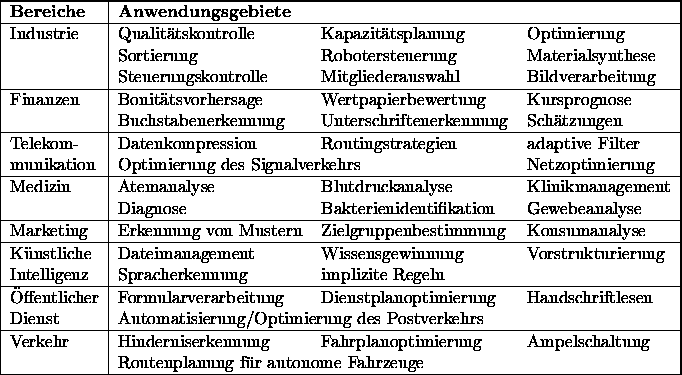
\includegraphics[width=0.8\textwidth]{../einleitung/bilder/einsatzKNN} 
% Bilddatei aus dem Unterverzeichnis bilder holen, skalieren auf 0.8*Satzspiegel
\caption{Anwendungsgebiete f�r den Einsatz von KNN, entnommen aus \url{http://vieta.math.tu-cottbus.de/~kolb/ml-nn/node10.html}}\label{einsatzKNN}
\end{figure}

\section{Begriffsdefinition}
\ac{KNN} sind die stark abstrahierte, technische Umsetzung der biologischen neuronalen Netze des menschlichen Gehirns. Mithilfe des Wissens �ber die Struktur und Funktionsweise vom Nervensystem k�nnen die biologischen Prinzipien der Informationsverarbeitung als systematisches Modell f�r den Rechner �bertragen werden.

\section{Zielsetzung}
Das Hauptziel dieser Arbeit ist es, dem Leser und Anwender einen leichten Einstieg in das Thema \ac{KNN} und deren Einsatzm�glichkeiten zu bieten. Damit wird dasselbe Ziel verfolgt, das schon Herr Koenecke mit seiner Arbeit hatte. Mit dem theoretischen Teil soll eine gewisse Wissensbasis �ber \ac{KNN} geschaffen werden. Beim praktischen Teil kann der Anwender mithilfe eines Programms, das durch den theoretischen Teil erworbene Wissen interaktiv veranschaulichen und verfestigen. Folgender Textauszug aus Herr Koeneckes Arbeit zeigt, was die Anforderungen an seinem geschriebenen Programm sind:

\emph{\glqq Die Grundidee besteht daraus, ein neuronales Netz zu implementieren, dessen Abl�ufe zu jeder Zeit angehalten und dessen interner Status eingesehen werden kann. �ber eine grafische Oberfl�che ist es dann m�glich, diese Funktionen aufzurufen, um das Netzwerk zu bedienen. W�hrenddessen k�nnen die internen Mechanismen beobachtet werden. So kann
ein Anwender testweise Eingaben t�tigen, deren Auswirkungen beobachten und daraus
Schl�sse ziehen. Die Interna des Netzwerks werden transparent. Anhand von bekannten
und interessanten Problemen kann sich so auch ein unerfahrener Nutzer die Funktionsweise
neuronaler Netze erschlie�en.\grqq} \citep[S. 7]{koenecke}

Weitestgehend sind die Anforderungen mit dem urspr�nglichen Programm erreicht worden. Ausgehend von diesem Programm als Basis sollen f�r diese Arbeit zwei gr��ere �nderungen stattfinden:


\begin{enumerate}\setlength{\itemsep}{0ex}
\item \emph{Portieren seines Programms komplett in Javascript, HTML und CSS}: Dies setzt voraus, dass die Berechnungen f�r das \ac{KNN} nicht mehr wie bisher im Hintergrund �ber einen Server laufen, sondern komplett lokal im Browser in Javascript durchgef�hrt werden. 
Von der Portierung ist zu erwarten, dass das Programm zwar nicht so schnell wie das urspr�ngliche Programm laufen wird, aber dennoch performant genug, dass es sich fl�ssig in einem aktuellen Browser benutzen l�sst.
\item \emph{�nderung des User Interfaces durch Hinzuf�gen spielerischer Elemente}: Die graphische Oberfl�che des Programms soll ver�ndert werden, sodass spielerische Interaktionen m�glich sind. Dabei ist es wichtig, dass das N�herbringen der Grundlagen von KNN immer noch im Vordergrund des Programms stehen soll. Daher sind die Ver�nderungen am Programm vor allem als Erweiterungen zu betrachten. Die Idee f�r die Erweiterungen fokussiert sich dabei auf den letzten Satz der oben von Herr Koenecke zitierten Textpassage, also die M�glichkeit anhand bekannter Probleme die Arbeitsweise \ac{KNN} zu erlernen. Im urspr�nglichen Programm ist der Anwender noch dazu gezwungen, sich die Probleme selbst herauszusuchen oder auszudenken. Um ihm diesen Schritt zu ersparen, soll es zus�tzlich eine Option vom Programm geben, anhand gestellter Aufgaben die Probleme kennenzulernen. Zum L�sen dieser Aufgaben, muss der Anwender die passenden Konfigurationen des \ac{KNN} vornehmen. So erh�lt der Anwender die M�glichkeit spielerisch zu erlernen, wie und wozu \ac{KNN} eingesetzt werden k�nnen.
\end{enumerate}

\section{Anmerkungen im Bezug auf Koeneckes Arbeit}
Zum Lesen dieser Arbeit soll keine zwingende Voraussetzung sein, Herrn Koeneckes Bachelorthesis durchzulesen. Daher werden sich einige �berschneidungen und Verweise zu Koeneckes Arbeit finden. Dies l�sst sich sowieso nicht komplett aufgrund der Tatsache vermeiden, dass diese Arbeit und der dazugeh�rige praktische Teil auf Grundlage seiner Arbeit und Anwendung entstanden ist. Die gr��ten �berschneidungen finden sich vor allem in den Kapiteln 2 - 5, in denen die Theorie behandelt wird, die mit der K�nstlichen Intelligenz und den \ac{KNN} in Verbindung stehen \citep[nachzulesen in seiner Thesis auf den Seiten S. 4-5 sowie 11-32]{koenecke}. Im Unterschied zu seiner Arbeit wurde die Theorie der KNN auf mehr Kapitel unterteilt und eine andere Strukturierung ausgew�hlt, mit dem Ziel eine bessere �bersicht �ber das Thema zu bieten. Ob dieser Weg wirklich der bessere ist, h�ngt im Grunde genommen vom Leser ab. Bevorzugt er es lieber kompakt in einem Kapitel sich die Theorie anzueignen, w�re die bessere Entscheidung sich Herr Koeneckes Arbeit durchzulesen. M�chte er lieber st�ckchenweise sich �ber verschiedene Kapitel die Theorie aneignen, kann diese Arbeit die bessere Wahl sein. 
%Vor allem richten sich diese Kapitel also an Leser, die seine Bachelorthesis noch nicht gelesen haben, nur wenig Wissen �ber \ac{KNN} haben und sich mit einem leichten Einstieg in das Thema zufrieden geben k�nnen. Genauso empfehlenswert sind sie f�r Leser, die ihr Wissen �ber \ac{KNN} noch einmal auffrischen wollen.

\section{Struktur dieser Arbeit}
\textcolor{red}{KOMMT AM ENDE}

\chapter{Grundlagen}\label{cGrundlagen} 
In diesem Kapitel soll eine grundlegende Wissensbasis zur Einordnung der Begriffe \ac{KI}, Maschinelles Lernen, Deep Learning und \ac{KNN} geschaffen werden. So kommt es bei Laien h�ufiger zu Verwechslungen dieser Begriffe, deswegen sollen in diesem Kapitel genauer auf sie eingegangen werden, bevor im Kapitel \ref{cKnn} der tiefere Einblick in die Theorie der \ac{KNN} erfolgt. Auf diese Weise l�sst sich besser verstehen, was \ac{KNN} sind und was sie nicht sind, f�r welchen Bereich sie eine Bedeutung spielen und wie sie in der Informatik einzuordnen sind. Es wird sich zeigen, dass das Thema \ac{KI} so breit gef�chert ist, dass f�r die Arbeit nur ein oberfl�chlicher Einschnitt in das Thema erfolgt. So werden vor allem die Grundlagen behandelt, die f�r die Thematik der \ac{KNN} und das im Rahmen der Bachelorthesis geschriebene Programm von Bedeutung sind.
Den Lesern, die tiefer in die Materie gehen m�chten, steht es nach der Einf�hrung mithilfe dieser Bachelorthesis offen, sich danach anderweitig �ber das Thema \ac{KI} zu informieren. 

\section{K�nstliche Intelligenz}

\subsection{Begriffserkl�rung}
Ob der Mensch ein Lebewesen oder eine Maschine f�r intelligent h�lt oder nicht, beruht meist auf seine relativ gute Intuition. So beurteilt er wie ausgepr�gt die kognitiven F�higkeiten sind, um sich an ungewohnte Situationen anzupassen. Aus wissenschaftlicher Sicht gibt es jedoch keine allgemein g�ltige Definition f�r den Begriff \emph{Intelligenz} \citep[S. 139]{rimscha}. \emph{\glqq Befragt man heute 20 Intelligenzforscher nach einer Definition, erh�lt man 20 unterschiedliche Antworten\grqq}, ist die Aussage von Thomas Gr�ter, einem Arzt und Sachbuchautor, der f�r die Neurophysiologie forschte \citep[S. 139]{hillmann}. Dass der Begriff Intelligenz schwer zu definieren ist, zeigt ebenfalls, wie schwierig es ist, die \ac{KI} zu definieren. Grob formuliert wird unter \ac{KI} \emph{die Nachbildung menschlicher Intelligenz durch Maschinen} verstanden(\textcolor{red}{Quelle nochmal raussuchen :P}). Dies betrifft auch die menschliche Wahrnehmung und das menschliche Handeln.

\subsection{Turing Test}
Um festzustellen, ob eine Maschine dem Anspruch der \ac{KI} gen�gt, hat Alan M. Turing als Vorschlag in seinem Paper \citep{turing} den nach ihm benannten Turing-Test ausgedacht. �ber l�ngere Zeit kommuniziert ein Mensch als Tester parallel mit zwei Gespr�chspartnern. Bei dem einen Gespr�chspartner handelt es sich um einen Menschen, bei dem anderen um eine Maschine. Die Kommunikation erfolgt ohne Sicht- und H�rkontakt (beispielsweise �ber ein Chat-Programm). Sowohl Mensch als auch Maschine versuchen den Tester zu �berzeugen, dass sie denkende Menschen sind. Kann der Tester nach der Unterhaltung nicht bestimmen, welcher von den Gespr�chspartnern die Maschine ist, gilt der Test als bestanden und die Maschine kann als intelligent bezeichnet werden. 

Bisherige Versuche diesen Test zu bestehen, gab es bereits mit Programmen wie \emph{ELIZA} (1966) oder dem Chatbot \emph{Eugene Goostman} (2014). Doch bei keinem dieser Versuche kann von Experten wirklich �berzeugt best�tigt werden, dass sie den Turing Test bestanden haben. Und trotz der intensiven Forschung im Bereich der \ac{KI} wird mit gro�er Wahrscheinlichkeit auch in absehbarer Zeit dies nicht passieren. 

\subsection{Starke und schwache \ac{KI}}
Aufgrund der Komplexit�t der \ac{KI} ist die Idee gekommen, eine Unterscheidung vorzunehmen \citep{russell-norvig}. Zum einen die \emph{starke \ac{KI}}, die dem Menschen ebenb�rtig ist und dazu imstande ist, komplexe kognitive Aufgaben autonom zu bew�ltigen, die sonst nur der Mensch l�sen kann. Zum anderen die \emph{schwache \ac{KI}}, die sich auf die L�sung der Probleme konzentriert, die konkretisiert und stark eingrenzt sind. In dieser Arbeit wird es ausschlie�lich um die L�sungsans�tze von Problemen aus dem Gebiet der schwachen \ac{KI} gehen. Beispielsweise z�hlen in das Gebiet der schwachen \ac{KI} Suchmaschinen, Spracherkennung und Bilderkennung, in denen in letzter Zeit beachtliche Erfolge erzielt werden konnten. Als Beispiele sind das 2014 von Amazon ver�ffentlichte, sprach-gesteuerte Ger�t Amazon Echo oder die Internet-Suchmaschine Google zu nennen. Sowohl die starke als auch die schwache \ac{KI} haben gemeinsam, dass bei beidem das Maschinelle Lernen eine immer gr��ere Bedeutung spielt. 

\section{Maschinelles Lernen}
\subsection{Begriffserkl�rung}
Beim Maschinellen Lernen (englisch: \emph{artificial intelligence - AI}) geht es um den Gewinn von Informationen und Wissen aus Erfahrung in Form von konkreten Beispieldaten \citep[ S. 143]{rimscha}. Im Gegensatz zur \emph{Symbolischen \ac{KI}} l�st der Computer also die Aufgabe nicht durch eine ihm vorher vorgegebene L�sungsvorschrift, sondern muss sich die L�sungsvorschrift selbst ableiten. Dadurch ist es f�r ihn auch m�glich, L�sungen f�r neue oder unbekannte Probleme zu finden. 

Die abgeleitete L�sungsvorschrift und damit die Ergebnisse dieser sind nur so gut, wie die Beispieldaten. Wenn die Beispieldaten nur einen bestimmten Bereich des Problems abdecken, aber nicht das Ganze, so werden die Daten als schlecht betrachtet. Um zu verdeutlichen, was damit gemeint ist, folgendes Beispiel: Es soll das Konsumverhalten von Pizza untersucht werden und es handelt sich bei den Testpersonen zuf�lligerweise um welche, die auf Di�t sind. Die Repr�sentativit�t der daraus entstehenden Ergebnisse wird unter diesen Bedingungen stark in Zweifel genommen werden k�nnen. Ebenfalls f�hren zu wenige zur Verf�gung stehende Daten zu schlechten Ergebnisse, deswegen k�nnen diese auch als schlechte Beispieldaten betrachtet werden. 

\subsection{Prinzip und Verfahren}

Das Maschinelle Lernen funktioniert im Grunde �hnlich wie das menschliche Lernen \citep{manhart}. So wird versucht, anhand der gegebenen Daten diese intelligent miteinander zu verkn�pfen, durch Ausprobieren und Abgleichen bestimmte Zusammenh�nge sowie Ergebnisse zu erschlie�en und anhand dieser Vorhersagen treffen zu k�nnen. Bei der Erkennung von Objekten auf Bildern lernt ein Mensch im Kindesalter zum Beispiel wie ein Hund aussieht, indem ihm Beispielbilder gezeigt werden, mit dem Hinweis, dass es sich um Hunde handelt. Auch beim Maschinellen Lernen f�ttert und trainiert der Programmierer das Lernprogramm mit Informationen in Form von Daten. Bei jeder Datei gibt er zus�tzlich an, ob es sich um einen Hund handelt oder nicht. Je mehr Beispieldaten das Programm bekommt, desto besser kann er unterscheiden, auf welchen Bildern Hunde zu sehen sind und auf welchen nicht. 

Um aus den Beispieldaten Wissen zu gewinnen, gibt es verschiedene Verfahren, die mathematische und statistische Algorithmen und Methoden verwenden. Davon nennenswerte w�ren zum Beispiel Entscheidungsb�ume, Reinforcement Learning, Genetische/Evolution�re Algorithmen, das Bayes'sche Lernen, der Monte Carlo Tree Search oder \ac{KNN}.\footnote{Die beiden letztgenannten Verfahren wurden unter anderem auch in dem von der Google-Tochter \emph{Deepmind} stammendem Programm \emph{Alpha Go} verwendet, der in der Lage war, im Mai 2017 den damaligen Weltranglistenersten \emph{Ke Jie} in drei von drei Go-Partien zu schlagen \citep{wunderlich}. Das ist insofern beachtlich, dass Go als sehr komplexes Brettspiel gilt. So bietet es mit ca. \( 2,08 \cdot 10^{170} \) m�glichen Stellungen sogar mehr als Schach mit $10^{43}$ m�glichen Stellungen.} Die verschiedenen Verfahren sind dabei nicht v�llig getrennt voneinander zu betrachten. Beispielsweise finden sich �berschneidungen zwischen genetischen Algorithmen und \ac{KNN}. Zudem sei zu erw�hnen, dass f�r die L�sung eines Problems auch oftmals nicht nur einer der Verfahren verwendet wird, sondern eine Kombination der verschiedenen Verfahren.

\section{Einordnung der KNN}
Anhand der vorherigen Erl�uterungen sollte nun klar zu unterscheiden sein, wie die verschiedenen Begriffe im Zusammenhang stehen. So sind \ac{KNN} ein Unterthema des Maschinellen Lernens, das wiederum ein Unterthema der \ac{KI} ist. Die Abbildung \ref{funktionLayer} soll diesen Zusammenhang veranschaulichen. 


\begin{figure}[!htb]
  \centering
	\begin{tikzpicture}
	\node[ellipse, minimum width=430, minimum height=180, thick, draw=black] (AI) at (0,10) {};
	\node[ellipse, minimum width=320, minimum height=150, thick, draw=black] (ML) at (-1.5,10) {};
	\node[ellipse, minimum width=200, minimum height=120, thick, draw=black] (NN) at (-3,10) {};
	\node[ellipse, minimum width=100, minimum height=90, thick, draw=black] (DL) at (-4.5,10) {};
	\node[above right = -1.7 and 0.3 of ML, text width=5cm,align=center, font=\large](){K�nstliche \\Intelligenz};
	\node[above right = -1.4 and -0.3 of NN, text width=5cm,align=center, font=\large](){Maschinelles \\Lernen};
	\node[above right = -0.1 and -0.9 of DL, text width=5cm,align=center, font=\large]() at(NN){Neuronale \\Netze};
	\node[text width=5cm,align=center, font=\large]() at(DL){Deep \\Learning};
	\end{tikzpicture}
	\caption{Venn Diagramm zur Einordnung der \ac{KNN}}
 	\label{funktionLayer}
\end{figure}

Der Vollst�ndigkeit halber erscheint im Diagramm auch der f�r die Arbeit relevante Begriff \emph{Deep Learning}. Bei Deep Learning handelt es sich um ein Teilgebiet der \ac{KNN}, die mit speziellen Formen von \ac{KNN} arbeiten. Um welche es sich dabei handelt, wird sp�ter im Abschnitt \textcolor{red}{noch erg�nzen} beschrieben.

\section{Bereiche der KNN}
Wie am Anfang des Kapitels \ref{c:einleitung} bereits erl�utert, werden \ac{KNN} in zahlreichen Anwendungsgebieten eingesetzt. Unterteilt werden kann dabei in zwei gro�e Bereiche \citep{rey_wender}. Zum einen die \emph{Modellierung menschlichen Verhaltens und Erlebens}, in der \ac{KNN} eingesetzt werden, um gewisse Gehirnprozesse zu simulieren und die Funktionsweise des Gehirns besser nachvollziehen zu k�nnen. Zum anderen die \emph{L�sung konkreter Anwendungsprobleme}, in der \ac{KNN} zur L�sung dieser in Bereichen wie der Statistik, Informatik, Wirtschaftswissenschaften eingesetzt werden. Die Arbeit wird sich vor allem mit den Problemstellungen des zweiten Bereiches besch�ftigen.

%%______________________________________
%
%
\newpage
\chapter*{Abk�rzungsverzeichnis}
\begin{acronym}{}
\acro{MLP}[MLP]{mehrlagige Perzeptron}
\acro{KI}[KI]{K�nstliche Intelligenz}
\acro{KNN}[KNN]{k�nstliche neuronale Netze}
\acro{GUI}[GUI]{Grafical User Interface}
\end{acronym}

%--------------------- VERZEICHNISSE ----------------

\listoffigures % Abbildungsverzeichnis erzeugen
\listoftables % Tabellenverzeichnis erzeugen

%--------------------- LITERATURLISTE ---------------
% Die Eintr�ge sollen alphabetisch sortiert sein.

\begin{thebibliography}{}

\bibitem[Bidelman(2010)]{bidelman} 
Bidelman, Eric: 
\emph{Web Worker-Grundlagen}, 
\url{https://www.html5rocks.com/de/tutorials/workers/basics/}, 26.07.2010, letzter Zugriff: 29. 08. 2017

\bibitem[Brij(2015)]{brij} 
Brij: 
\emph{Concurrency vs Multi-threading vs Asynchronous Programming : Explained}, 
\url{https://codewala.net/2015/07/29/concurrency-vs-multi-threading-vs-asynchronous-programming-explained/}, 29.07.2015, letzter Zugriff: 29. 08. 2017

\bibitem[Buckler(2013)]{buckler} 
Buckler, Craig: 
\emph{Implementing JavaScript Threading with Web Workers}, 
\url{https://www.safaribooksonline.com/blog/2013/10/24/implementing-javascript-threading-with-web-workers/}, 24.10.2013, letzter Zugriff: 29. 08. 2017

\bibitem[Corves(2005)]{corves} 
Corves, Anna: 
\emph{Nervenzellen im Gespr�ch}, 
\url{https://www.dasgehirn.info/grundlagen/kommunikation-der-zellen/nervenzellen-im-gespraech?gclid=COiWg7TdzNQCFU4W0wodK74IwA}, 2012, letzter Zugriff: 1. 07. 2017

\bibitem[Ertel(2016)]{ertel}
Ertel, Wolfgang: 
\emph{Grundkurs K�nstliche Intelligenz : Eine praxisorientierte Einf�hrung}, 4. Aufl., Berlin Heidelberg New York: Springer-Verlag, 2016

\bibitem[Hebb(1949)]{hebb}
Hebb, Donald Olding: 
\emph{The Organization Of Behavior: A Neuropsychological Theory}, Psychology Press edition 2002, 1949

\bibitem[Hillmann()]{hillmann} 
Hillmann, Leonard: 
\emph{Intelligentes Leben}, 
\url{http://www.tagesspiegel.de/themen/gehirn-und-nerven/gesund-leben-intelligentes-leben/13410564.html}, Ver�ffentlichkeitsdatum unbekannt, letzter Zugriff: 01.07.2017

\bibitem[Hoffmann(1993)]{hoffmann} 
Hoffmann, Norbert
\emph{Kleines Handbuch Neuronale Netze : Anwendungsorientiertes Wissen zum Lernen und Nachschlagen}, Berlin Heidelberg New York: Springer-Verlag, 1993

\bibitem[Koenecke(2016)]{koenecke}
Koenecke, Finn Ole: 
\emph{Realisierung eines interaktiven k�nstlichen neuronalen Netzwerks}, 2016

\bibitem[Kramer(2009)]{kramer}
Kramer, Oliver: 
\emph{Computational Intelligence : Eine Einf�hrung}, 1. Aufl., Berlin Heidelberg New York: Springer-Verlag, 2009.

\bibitem[Manhart (2017)]{manhart}
Manhart, Klaus: 
\emph{Was Sie �ber Maschinelles Lernen wissen m�ssen},
\url{https://www.computerwoche.de/a/was-sie-ueber-maschinelles-lernen-wissen-muessen,3329560}, 04.05.2017, letzter Zugriff: 02.07.2017

\bibitem[Minsky \& Papert(1969)]{minsky_papert}
Minsky, Marvin; Papert, Seymour:
\emph{Perceptrons: An Introduction to Computational Geometry}, 2nd edition with corrections, first edition 1969 , The MIT Press, Cambridge MA, 1972.

\bibitem[Rey \& Wender(1982)]{rey_wender}
Rey, G�nter Daniel ; Wender, Karl F.: 
\emph{Neuronale Netze : eine Einf�hrung in die Grundlagen, Anwendungen und Datenauswertung}, 2. vollst. �berarb. und erw. Aufl., Bern: Huber, 2011.

\bibitem[Riley(2017)]{riley}
Riley, Tonya: 
\emph{Artificial intelligence goes deep to beat humans at poker},
\url{http://www.sciencemag.org/news/2017/03/artificial-intelligence-goes-deep-beat-humans-poker}, 03.03.2017, letzter Zugriff: 07.07.2017

\bibitem[Rimscha(2014)]{rimscha}
Rimscha, Markus: 
\emph{Algorithmen kompakt und verst�ndlich : L�sungsstrategien am Computer}, 3. Aufl., Berlin Heidelberg New York: Springer-Verlag, 2014.

\bibitem[Russell \& Norvig(2010)]{russell-norvig}
Russell, Stuart ; Norvig, Peter:
\emph{Artificial Intelligence : A Modern Approach}, 3. Aufl(2010), London: Prentice Hall, 2010.

\bibitem[Scherer(1997)]{scherer}
Scherer, Andreas: Neuronale Netze : Grundlagen und Anwendungen. Berlin Heidelberg New York: Springer-Verlag, 1997.

\bibitem[SethBling(2015)]{sethBling}
SethBling: 
\emph{MarI/O - Machine Learning for Video Games},
\url{https://www.youtube.com/watch?v=qv6UVOQ0F44}, 13.06.2017, letzter Zugriff: 07.07.2017

\bibitem[Turing(1950)]{turing}
Turing, Alan M.: 
\emph{Computing Machinery and Intelligence}, Mind, 59, 1950.

\bibitem[Wolf(2009)]{wolf}
Wolf, J�rgen: 
\emph{C von A bis Z : das umfassende Handbuch},
\url{http://openbook.rheinwerk-verlag.de/c_von_a_bis_z/026_c_paralleles_rechnen_003.htm}  Bonn: Rheinwerk Verlag GmbH, 2009, letzter Zugriff: 29.08.2017

\bibitem[Wunderlich-Pfeiffer(2017)]{wunderlich}
Wunderlich-Pfeiffer, Frank : 
\emph{Alpha Go geht in Rente},
\url{https://www.golem.de/news/kuenstliche-intelligenz-alpha-go-geht-in-rente-1705-128059.html}, 29.05.2017, letzter Zugriff: 04.07.2017

\bibitem[Zell(1994)]{zell}
Zell, Andreas: 
\emph{Simulation neuronaler Netze}, 4.Auflage(2003) Deutschland: Oldenbourg Wissenschaftsverlag GmbH, 1994.

\end{thebibliography}
 
%\end{document} 
%% !TEX root = BachelorthesisNeu.tex
%%%%%%%%%%%%%%%%%%%%%%%%%%%%%%%%%%%%%%%%%%%%%%%%%%
%---- LaTeX-Header fuer Abschlussarbeiten, Prof. Thomas Goerne, Dez. 2012/Aug. 2013 ----
%%%%%%%%%%%%%%%%%%%%%%%%%%%%%%%%%%%%%%%%%%%%%%%%%

\documentclass[12pt,paper=A4,parskip=half, pointlessnumbers,bibtotoc,liststotoc,DIV=11,BCOR=1mm]{scrreprt}
% BCOR ist die Bindekorrektur (verlorener Rand am linken Blattrand)! Wert haengt von der Art der Heftung ab!!
% DIV ist eine Satzspiegeleinstellung von KOMA-Script / sccreprt.

\pagestyle{headings}

\usepackage[T1]{fontenc} % Font Encoding fuer europaeische Schriften mit Umlauten (Unterstuetzung der Worttrennung)
\usepackage{lmodern} % PostScript-Varianten der TeX Computer Modern-Schriften laden
\usepackage[english,ngerman]{babel} % Spracheinstellungen fuer Englisch und Neudeutsch laden

\usepackage{graphicx} % Grafikeinbindung (fuer .JPG, .JPEG, .PNG und .PDF, falls pdflatex benutzt wird)
\usepackage[table]{xcolor} % ermoeglicht farbige Schrift und farbige Tabellenzeilen
\definecolor{black}{gray}{0} % Umdefinition der Farbe black, falls noetig (0=schwarz, 1=weiss)
\definecolor{dblue}{rgb}{0.1,0.2,0.6} % Dunkelblau, fuer Hyperlinks
\definecolor{lgray}{gray}{0.9} % Hellgrau, fuer Tabellen (0=schwarz, 1=weiss)

\usepackage{booktabs} % fuer schoene Tabellen

\usepackage[round,authoryear]{natbib} % Literaturverweise mit Name/Jahreszahl in runden Klammern
\bibpunct[:\,]{(}{)}{,}{a}{}{,~}  % Feinformatierung der Natbib-Zitierweise

\usepackage[hyphens]{url}
\usepackage[colorlinks=true,linkcolor=black,citecolor=dblue,urlcolor=dblue]{hyperref} 
\usepackage{hyperref}  
% die Pakete url und hyperref ermoeglichen anklickbare URLs im Quellenverzeichnis in definierter Farbe, 
% sie ermoeglichen den Zeilenumbruch bei langen URLs, und sie erzeugen Hyperlinks (Farbe s.o.) 
% zwischen Quellenverweis und Quellenverzeichnis sowie zwischen label und ref im PDF-Dokument

% Fonteinstellungen fuer Bildunterschriften: Unterschrift serifenlos, "Abbildung" fett (bfseries = bold face series)
\setkomafont{captionlabel}{\sffamily\bfseries}
\setkomafont{caption}{\sffamily}

%---- eigene Packages ------
%\usepackage[usenames,dvipsnames,svgnames,table]{xcolor}
\usepackage{acronym}
\usepackage[latin1]{inputenc} % Inputencoding f�r PC/Win
\usepackage{tikz}
\usepackage{amsmath, amssymb}
\usepackage{mathtools}
\usepackage{pgffor}
\usepackage{varwidth}
\newcommand\Umbruch[2][3cm]{\begin{varwidth}{#1}\centering#2\end{varwidth}}
\usetikzlibrary{shapes,snakes}
\usetikzlibrary{positioning}
\usepgflibrary{arrows}
\usepackage{caption}
\usepackage{pgfplots}
\usepackage{subcaption}
\usepackage{xcolor}
\usepackage{listings}


\renewcommand{\thefootnote}{\roman{footnote}}
\newcommand{\net}{\operatorname{net}}


\colorlet{punct}{red!60!black}
\definecolor{background}{HTML}{EEEEEE}
\definecolor{delim}{RGB}{20,105,176}
\colorlet{numb}{magenta!60!black}

\lstdefinelanguage{json}{
    %basicstyle=\footnotesize\ttfamily,
    %numbers=left,
    %numberstyle=\scriptsize,
    %stepnumber=1,
    %numbersep=8pt,
    %showstringspaces=false,
    sensitive=false,
    %breaklines=true,
    %frame=lines,
    %backgroundcolor=\color{background},
    escapeinside={...a}{a...},
    literate=
     *{0}{{{\color{numb}0}}}{1}
      {1}{{{\color{numb}1}}}{1}
      {2}{{{\color{numb}2}}}{1}
      {3}{{{\color{numb}3}}}{1}
      {4}{{{\color{numb}4}}}{1}
      {5}{{{\color{numb}5}}}{1}
      {6}{{{\color{numb}6}}}{1}
      {7}{{{\color{numb}7}}}{1}
      {8}{{{\color{numb}8}}}{1}
      {9}{{{\color{numb}9}}}{1}
      {:}{{{\color{punct}{:}}}}{1}
      {,}{{{\color{punct}{,}}}}{1}
      {\{}{{{\color{delim}{\{}}}}{1}
      {\}}{{{\color{delim}{\}}}}}{1}
      {[}{{{\color{delim}{[}}}}{1}
      {]}{{{\color{delim}{]}}}}{1},
}

\definecolor{lightgray}{rgb}{.9,.9,.9}
\definecolor{darkgray}{rgb}{.4,.4,.4}
\definecolor{purple}{rgb}{0.65, 0.12, 0.82}

\lstdefinelanguage{JavaScript}{
  keywords={typeof, new, true, false, catch, function, return, null, catch, switch, var, if, in, while, do, else, case, break},
  keywordstyle=\color{blue}\bfseries,
  ndkeywords={class, export, boolean, throw, implements, import, this},
  ndkeywordstyle=\color{darkgray}\bfseries,
  identifierstyle=\color{black},
  sensitive=false,
  comment=[l]{//},
  morecomment=[s]{/*}{*/},
  commentstyle=\color{purple}\ttfamily,
  stringstyle=\color{red}\ttfamily,
  morestring=[b]',
  escapeinside={...a}{a...},
  morestring=[b]"
}

\lstset{
   language=JavaScript,
   backgroundcolor=\color{lightgray},
   extendedchars=true,
   basicstyle=\footnotesize\ttfamily,
   showstringspaces=false,
   showspaces=false,
   numbers=left,
   numberstyle=\footnotesize,
   numbersep=9pt,
   tabsize=2,
   breaklines=true,
   showtabs=false,
   captionpos=b
}



%------------------------------------------------------------------------------------------------------------------
%------ Eigenstaendigkeitserklaerung im gerahmten Kasten (parbox in einer framebox) ------
%------------------------------------------------------------------------------------------------------------------

\newcommand{\eigen}{
\setlength{\fboxsep}{2ex}
\setlength{\fboxrule}{0.8pt} 
% Einstellungen fuer Rahmenabstand und Rahmendicke der Framebox
\begin{center}
	\fbox{
		\parbox{0.8\linewidth}{
		Ich versichere, die vorliegende Arbeit selbstst\"andig ohne fremde Hilfe verfasst 
		und keine anderen Quellen und Hilfsmittel als die angegebenen benutzt zu haben. 
		Die aus anderen Werken w\"ortlich entnommenen Stellen oder dem Sinn nach 
		entlehnten Passagen sind durch Quellenangaben eindeutig kenntlich gemacht.
		\par\bigskip\bigskip\bigskip\bigskip
		\hspace*{0.8cm}Ort, Datum \hfill \vorname~\nachname\hspace*{0.8cm}
		}
	}
\end{center}
}

%%%%%%%%%%%%%%%%%%%%%%%%%%%%%%%%%%%%%%%%%%%%%%%%%
%
%\begin{document}
%%______________________________________


\chapter{Vorbild der KNN und das Prinzip eines k�nstlichen Neurons}\label{cKnn} 
%In diesem Kapitel soll als Einstieg erl�utert werden, in welchen Bereichen \ac{KNN} eingesetzt werden. Anschlie�end soll erl�utert werden, nach welchem Vorbild das Konzept der \ac{KNN} entstanden ist und wie sie nach diesem umgesetzt worden sind. 

\section{Nat�rliche neuronale Netze}
Das Besondere an KNN und was sie von anderen mathematischen Verfahren unterscheidet ist, dass sie urspr�nglich dem menschlichen Gehirn und den nat�rlichen neuronalen Netzen nachempfunden sind. Mit dem nat�rlichen Vorbild haben sie genau genommen jedoch kaum zu tun, da es nach aktuellem Stand noch unm�glich ist, komplett und korrekt die Eigenschaften der nat�rlichen neuronalen Netze in k�nstlicher Form abzubilden. Daher wird die folgende Darstellung der nat�rlichen neuronalen Netze stark vereinfacht sein, sodass noch deutlicher wird, inwiefern sich die KNN an ihnen orientieren.

Das menschliche Gehirn gilt als das komplexeste und vielschichtigste Organ in der ganzen Neurobiologie. Bekannt zu seinem Aufbau ist, dass es gesch�tzt 100 Milliarden \( (10^{11}) \) Neuronen bzw. Nervenzellen enth�lt, die alle zusammen ein Netzwerk bilden. Verkn�pft sind die Nervenzellen mit ca. \( 10^{14} \) - \(10^{15} \) synaptischen Verbindungen \citep[ S. 119-122]{kramer}. Eine Nervenzelle besteht aus einem Zellk�rper, vielen Dendriten und einem Axon (siehe Abb. \ref{neuronaufbau}). Die Dendriten sind daf�r zust�ndig Signale, die es von anderen Neuronen bekommt, aufzufangen und an den Zellk�rper hinzuleiten. Im Zellk�rper findet deren Verarbeitung statt. Wenn die Summe der empfangenen Signale, die die Nervenzelle von den anderen Nervenzellen bekommen hat, einen gewissen Schwellenwert der Erregung �berschreitet, wird ein elektrischer Impuls, das Aktionspotenzial, gesendet. Es wird dann gesagt, dass die Nervenzelle \emph{feuert} \citep[] {corves}. �ber das Axon wird dieser zu einer Synapse weitergeleitet. Bei einer Synapse handelt es sich um eine Verbindungsstelle zwischen zwei Nervenzellen, wodurch die �bertragung eines elektrischen Impulses von einer Nervenzelle zu einer anderen erm�glicht wird. Der elektrische Impuls sorgt daf�r, dass die andere Nervenzelle entweder gehemmt oder erregt wird.

%%Abbildung noch anpassen mit synapesen
%%
%----------- BILD ANFANG -------------
\begin{figure}[htp]     % h=here, t=top, b=bottom, p=page
	\centering
\includegraphics[width=0.8\textwidth]{../KNN/bilder/neuron} 
% Bilddatei aus dem Unterverzeichnis bilder holen, skalieren auf 0.8*Satzspiegel
\caption{Aufbau einer Nervenzelle}\label{neuronaufbau}
\end{figure}
%------------- BILD ENDE ---------------


\medskip
\section{Funktionsweise und Aufbau eines k�nstlichen Neurons}
KNN bestehen aus einer technischen Version der Nervenzellen, den \emph{k�nstlichen Neuronen}. Andere Bezeichnungen f�r Neuronen sind Units, Einheiten oder Knoten \citep[S.14]{rey_wender}. Ein einzelnes Neuron hat die einfache Aufgabe verschiedene Eingangssignale  aufzunehmen, diese zu verarbeiten und daraus ein Ausgangssignal auszugeben. Zur Veranschaulichung der damit verkn�pften mathematischen Zusammenh�nge, soll die Abbildung \ref{funktionNeuron} betrachtet werden. Die Nummerierung soll die Reihenfolge darstellen.

\begin{figure}
	\begin{tikzpicture}
	\tikzset{>=triangle 60}
	\node (rectInput) at (0,0.3) [draw,thick,minimum width=40,minimum height=120, rounded corners=6] {};
	\node (rectWeights) at (2,0.3) [draw,thick,minimum width=40,minimum height=120, rounded corners=6] {};
	\node (rectLayer) at (8,0.3) [draw,thick,minimum width=250,minimum height=120, rounded corners=3] {};
	
	% Annotate the outer Neuron Parameters
	\node[above of=rectInput, node distance=75, align=center, font=\footnotesize] () {Eingangs-\\werte};
	\node[above of=rectWeights, node distance=75, align=center, font=\footnotesize] () {Gewichte};
	\node[above of=rectLayer, node distance=75, align=center, font=\footnotesize] () {Neuron j};
	
	% Annotate the inner Neuron Parameters
	\def\y_t{1.9}
	\node (netj_t) at(5,\y_t) {Netzeingabe};
	\node[below = 0.5 of netj_t,font=\large] (netj) {${\net_j}$};
	\node[below = 0 of netj, font=\large] () {${=\net(j)}$};
	
	\node (akt_t) at(8,\y_t) {Aktivit�t};
	\node[below = 0.5 of akt_t, font=\large] (aj) {${a_j}$};
	\node[below = 0 of aj, font=\large] () {${=\varphi(\net_{j})}$};
	\draw (6.5,\y_t + 0.5) -- (6.5,\y_t - 3.7);
	
	\node (aus_t) at(11,\y_t) {Ausgabe};
	\node[below = 0.5 of aus_t, font=\large] (oj) {${o_j}$};
	\node[below = 0 of oj, font=\large] () {$={f_{\mathrm{out}}(a_{j})}$};
	\draw (9.5,\y_t + 0.5) -- (9.5,\y_t - 3.7);
	
	
	% Draw the input layer nodes with arrows to netj
	\def\cInputNodes{2}
    \foreach \name / \y in {0,...,\numexpr\cInputNodes-1\relax}
    	\node[font=\large](I\y) at (0,-\y*1.2+1.9 ) {${x_\y}$}; 
    \foreach \name / \y in {0,...,\numexpr\cInputNodes-1\relax}{
    	\draw[shorten >=87,shorten <=1,->](I\y) -> (6.5, 0.5) 
    	node [pos=0.255, above=-0.1, font=\large] {${w_{\y j}}$};
    }
    
    \node[font=\large](I-\cInputNodes) at (0,-2*1.2+1.1) {${x_n}$};
    \draw[shorten >=87,shorten <=1,->](I-\cInputNodes) -> (6.5, 0.5) 
    node [pos=0.255, above=-.07, font=\large] {${w_{nj}}$};  
    
    \node [right = 5 of rectLayer](aus_end){};
    \draw[shorten >=87,shorten <=0.9,->] (rectLayer) -- (aus_end)
    node [pos=0.2, above=-.07, font=\large] {${o_{j}}$};
    
    % Ordernumber of the steps   , color={rgb:red,1;green,2;blue,5}
    \tikzstyle{nrNode}=[font=\Large, circle, radius=2.5,draw]
    \node[below = 0.5 of rectInput, nrNode] () {1};
    \node[below = 0.5 of rectWeights, nrNode] () {2};
    \node[below = 0.5 of rectLayer, nrNode] (n4) {4};
    \node[left = 2 of n4, nrNode] () {3};
    \node[right = 2 of n4, nrNode] () {5};
    
	\end{tikzpicture}
	\caption{Funktionsweise eines Neurons, modifizierte Version aus \url{http://www.codeplanet.eu/tutorials/csharp/70-kuenstliche-neuronale-netze-in-csharp.html}}
 	\label{funktionNeuron}
\end{figure}

Es soll $i,j,n \in \mathbb{N}$ gelten.
\begin{enumerate}\setlength{\itemsep}{0ex}
\item Ist $n$ die Anzahl der Eingaben, so bekommt das Neuron $j$ die Eingangssignale beziehungsweise \emph{Eingangswerte} $x_1$ bis $x_n$ (biologische Analogie: Dendriten). Die Eingangswerte stammen entweder von anderen Neuronen oder Reizen aus der Umwelt.
\item Die \emph{Gewichte} (engl. \emph{weights}) $w_{ij}$ stehen f�r die St�rke der Verbindungen (biologische Analogie: Synapse) vom Sender Neuron $i$ zum Empf�nger Neuron $j$. Durch sie wird bestimmt, zu welchem Grad die empfangenen Eingangswerte Einfluss auf die sp�tere Aktivierung des Neurons $j$ nehmen werden. Je nach Vorzeichen werden die Eingangssignale jeweils verst�rkt oder geschw�cht. 
\item Die \emph{Netzeingabe} $\net_j$ verarbeitet die erhaltenen Informationen (also die Eingangssignale und die dazu geh�rigen Gewichtungen) und berechnet sich mithilfe der �bertragungsfunktion $\net(j)$ (auch Propagierungs- oder Netzeingabefunktion genannt).
\item Der \emph{Aktivit�tslevel} $a_{j}$ beschreibt den aktuellen Zustand des Neurons $j$ und berechnet sich aus der Netzeingabe mithilfe der Aktivierungsfunktion $\varphi(\net_{j})$ (auch Aktivit�tsfunktion genannt). 
\item Die \emph{Ausgabe} $o_j$ berechnet sich mithilfe der Ausgabefunktion $f_\text{out}(a_{j})$. Sie ist der Wert, der entweder sp�ter anderen Neuronen als Eingabe gesendet wird oder einen Ausgabewert des KNN darstellt.
\end{enumerate}

\subsection{�bertragungsfunktion}
Die am h�ufigsten verwendete �bertragungsfunktion ist die Linearkombination, bei der die Eingangssignale $x_1$ bis $x_n$ mit den Gewichten $w_{1j}$ bis $w_{nj}$ multipliziert werden und alle Produkte aufsummiert werden (siehe Gl. \ref{eq:net_j}). Daher wird f�r die �bertragungsfunktion h�ufig als Symbol $\sum$ verwendet.
\begin{equation}
	\net_j = \net(j) =\sum_{i=0}^n x_{i}w_{ij}
   \label{eq:net_j}
\end{equation}

\subsection{Aktivierungsfunktion}
In der Literatur sind zahlreiche Beispielfunktionen zu finden, die sich als Aktivierungsfunktion nutzen lassen. In den Tabellen \ref{t_actFunc} und \ref{t_actFunc2} sind die Aktivierungsfunktionen aufgef�hrt, die h�ufig zu finden sind.
%----------- TABELLE START -------------
\begin{table}[htp] 
\centering
\begin{tabular}{p{5cm}|p{5cm}|p{5cm}}  % Spalten nach Ausrichtung: l, c, r, p{breite}, mit zwei vertikalen Spaltentrennern
%bitte nicht das kleine L "l" und den Vertikalstrich "|" verwechseln!!! :)
% kleines L steht f�r eine linksb�ndige Spalte, Vertikalstrich erzeugt eine Trennlinie zwischen zwei Spalten

%\multicolumn{2}{c}{\large\bfseries Erste Bundesliga, Spielzeit 2011/2012}\\ \midrule
 {\bfseries {Lineare Aktivierungsfunktion}} & {\bfseries {ReLu (Rectified Linear Unit)}}  & {\bfseries {Bin�re Aktivierungsfunktion}}\\ \hline
  
  %%Erste Zeile
Linearer Zusammenhang zwischen dem Netzinput $\net_j$ und dem Aktivit�tslevel $a_j$. Weder nach unten noch nach oben ist der Wertebereich f�r den Aktivit�tslevel beschr�nkt.
	& Lineare Aktivierungsfunktion mit Schwelle 0. Es ist erforderlich, dass die festgelegte Schwelle 0 �berschritten wird, erst dann ist der Zusammenhang zwischen den beiden Gr��en linear.
	& H�ufig wird diese Funktion auch Heavyside-Funktion, Schwellenwertfunktion oder Schrittfunktion genannt. Der Aktivit�tslevel kann lediglich zwei Zust�nde annehmen, n�mlich 0 (in manchen F�llen auch -1) oder +1. \\ \hline


%%Zweite Zeile
\large $a_j=m\cdot \net_j + b$
	&\large	$a_j=\max(0,\net_j)$
	& \large $a_j =
  \small\begin{cases}
     1  & \quad \text{falls } \net_j \geq 0\\
    0  & \quad \text{falls } \net_j < 0\\
  \end{cases}
$ \\ \hline

%%Dritte Zeile
%draw a grid in the x-y plane
\begin{tikzpicture}
\captionsetup{labelformat=empty}
\def\ymax{2}
\def\xmax{2}
	%  \node[anchor=south] at (0,0) {\includegraphics[width=\textwidth]{mein_bild.jpg}};
% Feine Hilfslinien
x=1cm, y=1cm,  scale=1.0, 
font=\footnotesize,
>=latex   %Voreinstellung f�r Pfeilspitzen

% Gitternetzlinien
\draw[xstep=0.5cm, ystep=0.5cm, very thin, color=lightgray] (-\xmax-0.5,-\ymax-0.5) grid (\xmax+0.5,\ymax+0.5);

% x-Achse
\draw[->] (-\xmax-0.5,0) -- (\xmax+0.5,0) node[above left] {$\net_j$}; 
%Zahlen auf x-Achse
\foreach \x in {-\xmax,...,-1,1,2,...,\xmax}
\draw[shift={(\x,0)},color=black] (0pt,2pt) -- (0pt,-2pt) node[below] {\footnotesize $\x$};

% y-Achse 
\draw[->] (0,-\ymax-0.5) -- (0,\ymax+0.5) node[right] {$a_j$};%node[above left]
%Zahlen auf y-Achse
\foreach \y in {-\ymax,...,-1,1,2,...,\ymax}
\draw[shift={(0,\y)},color=black] (2pt,0pt) -- (-2pt,0pt) node[left] {\footnotesize $\y$};

%Ursprung
\draw[color=black] (0pt,-5pt) node[right] {\footnotesize $0$};

\draw[scale=1,domain=-\xmax-0.5:\xmax+0.5,smooth,variable=\x,blue] plot ({\x},{\x});

\end{tikzpicture}
\captionsetup{labelformat=empty}
\caption*{mit $m=1$ und $b=0$}
%erster Graph ENDE LA

	& %zweiter Graph
\begin{tikzpicture}
\def\ymax{2}
\def\xmax{2}
	%  \node[anchor=south] at (0,0) {\includegraphics[width=\textwidth]{mein_bild.jpg}};
% Feine Hilfslinien
x=1cm, y=1cm,  scale=1.0, 
font=\footnotesize,
>=latex   %Voreinstellung f�r Pfeilspitzen

% Gitternetzlinien
\draw[xstep=0.5cm, ystep=0.5cm, very thin, color=lightgray] (-\xmax-0.5,-\ymax-0.5) grid (\xmax+0.5,\ymax+0.5);

% x-Achse
\draw[->] (-\xmax-0.5,0) -- (\xmax+0.5,0) node[above left] {$\net_j$}; 
%Zahlen auf x-Achse
\foreach \x in {-\xmax,...,-1,1,2,...,\xmax}
\draw[shift={(\x,0)},color=black] (0pt,2pt) -- (0pt,-2pt) node[below] {\footnotesize $\x$};

% y-Achse 
\draw[->] (0,-\ymax-0.5) -- (0,\ymax+0.5) node[right] {$a_j$};%node[above left]
%Zahlen auf y-Achse
\foreach \y in {-\ymax,...,-1,1,2,...,\ymax}
\draw[shift={(0,\y)},color=black] (2pt,0pt) -- (-2pt,0pt) node[left] {\footnotesize $\y$};

%Ursprung
\draw[color=black] (0pt,-5pt) node[right] {\footnotesize $0$};


\draw[scale=1,domain=0:\xmax+0.5,smooth,variable=\x,blue] plot ({\x},{\x});
\end{tikzpicture} 
%zweiter Graph ENDE RELU

	& %dritter Graph
\begin{tikzpicture}
\def\ymax{2}
\def\xmax{2}
	%  \node[anchor=south] at (0,0) {\includegraphics[width=\textwidth]{mein_bild.jpg}};
% Feine Hilfslinien
x=1cm, y=1cm,  scale=1.0, 
font=\footnotesize,
>=latex   %Voreinstellung f�r Pfeilspitzen

% Gitternetzlinien
\draw[xstep=0.5cm, ystep=0.5cm, very thin, color=lightgray] (-\xmax-0.5,-\ymax-0.5) grid (\xmax+0.5,\ymax+0.5);

% x-Achse
\draw[->] (-\xmax-0.5,0) -- (\xmax+0.5,0) node[above left] {$\net_j$}; 
%Zahlen auf x-Achse
\foreach \x in {-\xmax,...,-1,1,2,...,\xmax}
\draw[shift={(\x,0)},color=black] (0pt,2pt) -- (0pt,-2pt) node[below] {\footnotesize $\x$};

% y-Achse 
\draw[->] (0,-\ymax-0.5) -- (0,\ymax+0.5) node[right] {$a_j$};%node[above left]
%Zahlen auf y-Achse
\foreach \y in {-\ymax,...,-1,1,2,...,\ymax}
\draw[shift={(0,\y)},color=black] (2pt,0pt) -- (-2pt,0pt) node[left] {\footnotesize $\y$};

%Ursprung
\draw[color=black] (0pt,-5pt) node[right] {\footnotesize $0$};


\draw[scale=1,domain=-2.5:0,smooth,variable=\x,blue] plot ({\x},0);
\draw[scale=1,domain=0:2.5,smooth,variable=\x,blue] plot ({\x},1);
\end{tikzpicture}
%dritter Graph ENDE bin�r

\end{tabular}
\caption{lineare Aktivierungsfunktion, ReLu und die bin�re Aktivierungsfunktion}\label{t_actFunc}

\end{table}
%--------- TABELLE ENDE ---------------















%%DRITTE TABELLE
%----------- TABELLE START -------------
\begin{table}[htp] 
\centering
\begin{tabular}{p{7cm}|p{7cm}}  % Spalten nach Ausrichtung: l, c, r, p{breite}, mit zwei vertikalen Spaltentrennern
%bitte nicht das kleine L "l" und den Vertikalstrich "|" verwechseln!!! :)
% kleines L steht f�r eine linksb�ndige Spalte, Vertikalstrich erzeugt eine Trennlinie zwischen zwei Spalten

%\multicolumn{2}{c}{\large\bfseries Erste Bundesliga, Spielzeit 2011/2012}\\ \midrule
 {\bfseries {Logistische Aktivierungsfunktion}} & {\bfseries {Tangens Hyperbolicus Aktivierungsfunktion}}\\ \hline
  
  %%Erste Zeile
Der Wertebereich ist auf 0 bis +1 begrenzt. Werden gro�e negative Werte (z.B. -100) f�r $\net_j$ eingesetzt, ist der Aktivit�tslevel nahe 0. Mit zunehmenden Netzinput steigt der Graph zun�chst langsam, wird dann immer steiler (sodass er dabei zwischenzeitlich einer linearen Funktion gleicht) und n�hert sich daraufhin wieder asymptotisch dem Wert +1 an. 
& Diese Funktion wird h�ufig abgek�rzt $\tanh$ Aktivierungsfunktion genannt und verl�uft �hnlich wie die logistische Aktivierungsfunktion. Der Unterschied besteht jedoch vor allem darin, dass der Wertebereich zwischen -1 und +1 liegt.\\ \hline

%%Zweite Zeile
\large $a_j=$\Large{$\frac{1}{1+e^{-k\net_j}}$} &  \large $a_j=$\Large{$\frac{e^{\net_j}-e^{-\net_j}}{e^{\net_j}+e^{-\net_j}}$}\\ \hline

%%Dritte Zeile
%draw a grid in the x-y plane
\centering
\begin{tikzpicture}
\def\ymax{2}
\def\xmax{2}
	%  \node[anchor=south] at (0,0) {\includegraphics[width=\textwidth]{mein_bild.jpg}};
% Feine Hilfslinien
x=1cm, y=1cm,  scale=1.0, 
font=\footnotesize,
>=latex   %Voreinstellung f�r Pfeilspitzen

% Gitternetzlinien
\draw[xstep=0.5cm, ystep=0.5cm, very thin, color=lightgray] (-\xmax-0.5,-\ymax-0.5) grid (\xmax+0.5,\ymax+0.5);

% x-Achse
\draw[->] (-\xmax-0.5,0) -- (\xmax+0.5,0) node[above] {$\net_j$}; 
%Zahlen auf x-Achse
\foreach \x in {-\xmax,...,-1,1,2,...,\xmax}
\draw[shift={(\x,0)},color=black] (0pt,2pt) -- (0pt,-2pt) node[below] {\footnotesize $\x$};

% y-Achse 
\draw[->] (0,-\ymax-0.5) -- (0,\ymax+0.5) node[right] {$a_j$};%node[above left]
%Zahlen auf y-Achse
\foreach \y in {-\ymax,...,-1,1,2,...,\ymax}
\draw[shift={(0,\y)},color=black] (2pt,0pt) -- (-2pt,0pt) node[left] {\footnotesize $\y$};

%Ursprung
\draw[color=black] (0pt,-5pt) node[right] {\footnotesize $0$};

\draw[scale=1,domain=-\xmax-0.5:\xmax+0.5,smooth,variable=\x,blue] plot ({\x},{1/(1+exp(-1*\x))});
\end{tikzpicture} 
\caption*{mit $k = 1$}
& 
%dritter Graph
{\centering
\begin{tikzpicture}

\def\ymax{2}
\def\xmax{2}
	%  \node[anchor=south] at (0,0) {\includegraphics[width=\textwidth]{mein_bild.jpg}};
% Feine Hilfslinien
x=1cm, y=1cm,  scale=1.0, 
font=\footnotesize,
>=latex   %Voreinstellung f�r Pfeilspitzen

% Gitternetzlinien
\draw[xstep=0.5cm, ystep=0.5cm, very thin, color=lightgray] (-\xmax-0.5,-\ymax-0.5) grid (\xmax+0.5,\ymax+0.5);

% x-Achse
\draw[->] (-\xmax-0.5,0) -- (\xmax+0.5,0) node[above] {$\net_j$}; 
%Zahlen auf x-Achse
\foreach \x in {-\xmax,...,-1,1,2,...,\xmax}
\draw[shift={(\x,0)},color=black] (0pt,2pt) -- (0pt,-2pt) node[below] {\footnotesize $\x$};

% y-Achse 
\draw[->] (0,-\ymax-0.5) -- (0,\ymax+0.5) node[right] {$a_j$};%node[above left]
%Zahlen auf y-Achse
\foreach \y in {-\ymax,...,-1,1,2,...,\ymax}
\draw[shift={(0,\y)},color=black] (2pt,0pt) -- (-2pt,0pt) node[left] {\footnotesize $\y$};

%Ursprung
\draw[color=black] (0pt,-5pt) node[right] {\footnotesize $0$};


\draw[scale=1,domain=-\xmax-0.5:\xmax+0.5,smooth,variable=\x,blue] plot ({\x},{(exp(\x)-exp(-\x))/(exp(\x)+exp(-\x))});
\end{tikzpicture}\caption*{mit $\theta_j = 0$}
%dritter Graph ENDE bin�r
\par}\\ \hline
\multicolumn{2}{c}{}\\
\multicolumn{2}{l}{Dabei gilt:}\\
\multicolumn{2}{l}{$m$ = Steigung der Geraden}\\
\multicolumn{2}{l}{$b$ = Achsenschnittpunkt der Geraden}\\
\multicolumn{2}{l}{$k$ = konstanter Faktor}\\

\end{tabular}
\caption{Logistische und $\tanh$ Aktivierungsfunktion}\label{t_actFunc2}

\end{table}
%--------- TABELLE ENDE ---------------

�fters wird f�r die Aktivierungsfunktion (vor allem f�r die bin�re Aktivierungsfunktion) ein bestimmter Schwellenwert $\theta_j$ f�r das Neuron $j$ mitber�cksichtigt. Bevor das Neuron aktiviert wird, muss noch zus�tzlich der Schwellenwert �berschritten werden. Bei der Berechnung der Aktivierung kommt als zus�tzlicher Schritt, dass der Schwellenwert von der Netzeingabe abgezogen wird (siehe Gl. \ref{eq:actFunc_Schw}).
\begin{equation}
a_j=\varphi(\net_j - \theta_j)\label{eq:actFunc_Schw}
\end{equation}
Welche Aktivierungsfunktion gew�hlt wird, h�ngt von der Art des \ac{KNN} bzw. vom konkreten Anwendungsproblem ab. Im Kapitel \ref{c:aktivierungsfunktion_lernen} soll nochmal darauf eingegangen werden.


\subsection{Ausgangsfunktion}
Bei nat�rlichen Neuronen ist es erforderlich, dass der Aktivit�tslevel eine bestimmte Schwelle �berschreitet, bevor das Neuron feuert. Diese Bedingung haben k�nstliche Neuronen nicht, daf�r wird aber verlangt, dass der Ausgang mit zunehmender Aktivit�t nicht kleiner wird, d.h. die Ausgangsfunktion hat die Anforderung \emph{monoton wachsend} zu sein. F�r bestimmte Arten von \ac{KNN} wie den hybriden Netzen ist eine klare Trennung zwischen der Aktivierungsfunktion und der Ausgangsfunktion erforderlich. In zahlreicher Literatur jedoch wird die Ausgangsfunktion von den Autoren als Bestandteil der Aktivierungsfunktion angesehen und daher gar nicht erw�hnt. Im Grunde genommen wird dann also f�r die Ausgangsfunktion die Identit�tsfunktion (siehe Gl. \ref{eq:fout_id}) eingesetzt, auch f�r diese Arbeit soll sie verwendet werden. 

\begin{equation}
	o_j=f_{\mathrm{out}(a_j)} = a_j
   \label{eq:fout_id}
\end{equation}


\chapter{Struktur der KNN}
\section{Aufbaustruktur}
Der Aufbau eines KNN l�sst sich als ein Netz k�nstlicher Neuronen beschreiben, die im Prinzip beliebig �ber gerichtete und gewichtete Verbindungen miteinander verkn�pft sind. Als Netzwerkgraph kann das so aussehen, dass dessen Knoten die Neuronen und die Kanten die Verbindungen repr�sentieren sollen. Aufgrund dieser Darstellungsm�glichkeit kann die mathematische Definition von \ac{KNN} folgenderma�en lauten: Ein KNN \emph{\glqq besteht aus einer Menge von Neuronen $N=\lbrace n_1, \dotsc, n_m\rbrace$ und einer Menge von Kanten $K=\lbrace k_1, \dotsc, k_p\rbrace$ mit $K \subset N \times N$\grqq} \citep[S.54]{scherer}.

Die Struktur und Anordnung der k�nstlichen Neuronen innerhalb des \ac{KNN} wird als \emph{Topologie} definiert. Welche Topologie verwendet werden soll, h�ngt vom konkreten Anwendungsproblem ab. Es lassen sich zwei Grundtypen von Netzen unterscheiden:
\begin{itemize} 
\item Zum einen die \emph{r�ckgekoppelten Netze} (bzw. \emph{rekurrente Netzwerke} oder \emph{Feedback Netzwerke)}, bei denen die Ausgabewerte auf die Eingabe zur�ckgef�hrt werden k�nnen. Die Verbindungen k�nnen also in beide Richtungen verlaufen. 
\item Zum anderen die \emph{vorw�rts gerichteten Netze} (bzw. \emph{Feedforward Netzwerke)}, dessen berechneten Ausgabewerte keinen Einfluss auf die Eingabe haben. Hier k�nnen die Verbindungen also nur in eine Richtung gehen, n�mlich von der Eingabe zur Ausgabe.
\end{itemize} 

%%Beispiel Feedforward Netzwerk
\begin{figure}[htp]
\centering
\begin{minipage}[b]{.45\textwidth}
	\centering
	\def\layersep{4cm}
	\begin{tikzpicture}[shorten >=1pt,->,draw=black!50, node distance=\layersep]
	    \tikzstyle{every pin edge}=[<-,shorten <=1pt, ultra thick]
	    \tikzset{>=latex} 
	    \tikzstyle{neuron}=[circle,fill=black!55,minimum size=22pt,inner sep=0pt]
	    \tikzstyle{input neuron}=[neuron];
	    \tikzstyle{output neuron}=[neuron];
	    \tikzstyle{hidden neuron}=[neuron];
	    \tikzstyle{annot} = [text width=4em, text centered]
	
	    % Draw the input layer nodes
	    \foreach \name / \y in {1,...,3}
	    % This is the same as writing \foreach \name / \y in {1/1,2/2,3/3,4/4}
	        \node[input neuron] (I-\name) at (0,-\y*1.5) {};
	
	    % Draw the hidden layer nodes
	    \foreach \name / \y in {1,...,3}
	        \path[yshift=-0cm]
	            node[hidden neuron] (H-\name) at (\layersep,-\y*1.5 cm) {};
	
	    % Connect every node in the input layer with every node in the
	    % hidden layer.
	    \foreach \source in {1,...,3}
	        \foreach \dest in {1,...,3}
	            \path (I-\source) edge[line width=2pt, color=black] (H-\dest);
	
	    
	    % Annotate the neurons
	    \tikzset{every pin edge/.style={draw=red, ultra thick}}
	   
	\end{tikzpicture}\captionsetup{format=plain}\caption{Schematisches Beispiel Feedforward Netzwerk}\label{abb:feedforwardNetz}
%%Beispiel Feedback Netzwerk
\end{minipage}
\begin{minipage}[b]{.45\textwidth}
	\centering
	\def\layersep{4cm}
	\begin{tikzpicture}[shorten >=1pt,->,draw=black!50, node distance=\layersep]
	    \tikzstyle{every pin edge}=[<-,shorten <=1pt, ultra thick]
	    \tikzset{>=latex} 
	    \tikzstyle{neuron}=[circle,fill=black!55,minimum size=22pt,inner sep=0pt]
	    \tikzstyle{input neuron}=[neuron];
	    \tikzstyle{output neuron}=[neuron];
	    \tikzstyle{hidden neuron}=[neuron];
	    \tikzstyle{annot} = [text width=4em, text centered]
	
	    % Draw the input layer nodes
	    \foreach \name / \y in {1,...,3}
	    % This is the same as writing \foreach \name / \y in {1/1,2/2,3/3,4/4}
	        \node[input neuron] (I-\name) at (0,-\y*1.5) {};
	
	    % Draw the hidden layer nodes
	    \foreach \name / \y in {1,...,2}
	        \path[yshift=-1cm]
	            node[hidden neuron] (H-\name) at (\layersep,-\y*1.5 cm) {};
	
	    % Connect every node in the input layer with every node in the
	    % hidden layer.
	    \foreach \source in {1,...,3}
	        \foreach \dest in {1,...,2}
	            \path (I-\source) edge[line width=2pt, color=black] (H-\dest);
	
	    
	    % Annotate the neurons
	    \tikzset{every pin edge/.style={draw=red, ultra thick}}
	    \path (H-2) edge [out=330,in=10,looseness=8, line width=2pt, color=black] node[above]{}(H-2);
	    \path (H-1) edge [out=30,in=30, line width=2pt, color=black] node[above]{}(I-1);
	   
	\end{tikzpicture}
	\captionsetup{format=plain}\caption{Schematisches Beispiel Feedback Netzwerk}\label{feedbackNetz}
	\end{minipage}
\end{figure}

Auf erstere soll nicht mehr n�her eingegangen werden, zwar sind sie aufgrund ihrer gr��eren Leistungsf�higkeit im Vergleich zu den vorw�rts gerichteten Netzen interessanter, doch daf�r deutlich komplexer. 

Bei den Feedforward Netzwerken k�nnen drei verschiedene Arten von Neuronen klassifiziert werden:
\begin{itemize}
\item Zum einen gibt es die \emph{Input-Neuronen} (bzw. \emph{Eingangsneuronen}), die Eingabesignale von der Au�enwelt zum Beispiel in Form von Reizen und Mustern bekommen. 
\item Desweiteren gibt es die \emph{Hidden-Neuronen}, die zwischen den Input- und Output-Neuronen stehen. 
\item Als letztes sind die \emph{Output-Neuronen} (bzw. \emph{Ausgangsneuronen}) aufzuf�hren, die die Aufgabe haben, Signale an die Au�enwelt auszugeben und auszuwirken. 
\end{itemize} 
H�ufig sind bei Feedforward Netzwerken die Neuronen in mehrere \emph{Schichen} %(bzw. \emph{Gruppen} oder \emph{Lagen}) 
  eingeteilt. Es gibt keine verbindlichen Regeln f�r die Einteilung eines Netzes in Schichten, f�r gew�hnlich werden die Neuronen zusammengefasst, die gemeinsam eine bestimmte Aufgabe durchf�hren. Beispielsweise bei der Abbildung \ref{ffNetz_Aufbau} ist das Kriterium f�r die Einteilung die Verbindungen der Neuronen. Dabei lassen sich die Input-Neuronen 1,...,3 zur Eingabeschicht und die Neuronen 11 und 12 zur Ausgabeschicht zusammenfassen. Dazwischen bilden die Neuronen 4,...,7 und die Neuronen 8,...,10 jeweils eine versteckte Schicht. %Es handelt sich in dem Beispiel um ein vierschichtiges Netz. 
\begin{figure}[htp]
	\def\layersep{3cm}
	\begin{tikzpicture}[shorten >=1pt,->,draw=black!50, node distance=\layersep]
	    \tikzstyle{every pin edge}=[<-,shorten <=1pt]
	    \tikzstyle{neuron}=[circle,fill=black!25,minimum size=17pt,inner sep=0pt]
	    \tikzstyle{input neuron}=[neuron, fill=green!50];
	    \tikzstyle{output neuron}=[neuron, fill=red!50];
	    \tikzstyle{hidden neuron}=[neuron, fill=blue!50];
	    \tikzstyle{annot} = [text width=4em, text centered]
	
	    % Draw the input layer nodes
	    \foreach \name / \y in {1,...,3}
	    % This is the same as writing \foreach \name / \y in {1/1,2/2,3/3,4/4}
	        \node[input neuron, pin=left:Input $x_\y$] (I-\name) at (0,-\y) {\y};
	
	    % Draw the hidden layer nodes
	    \foreach \name / \y in {1,...,4}{
	    	\pgfmathtruncatemacro\ynew{\y+3}
	        \path[yshift=0.5cm]
	            node[hidden neuron] (H-\name) at (\layersep,-\y cm) {\ynew};
	    }
	            
	    % Draw the hidden layer nodes 2
	    \foreach \name / \y in {1,...,3}
	    	\pgfmathtruncatemacro\ynew{\y+7}
	        \path node[hidden neuron] (H2-\name) at (\layersep*2,-\y cm) {\ynew};
	
	    % Draw the output layer node
	    %\node[output neuron,pin={[pin edge={->}]right:Output}, right of=H-3] (O) {};
	    \foreach \name / \y in {1,...,2}
	    	\pgfmathtruncatemacro\ynew{\y+10}
	        \path[yshift=-0.5cm]
	    	node[output neuron, ,pin={[pin edge={->}]right:Output $o_{\y}$}] (O-\name) at (\layersep*3,-\y cm) {\ynew};
	
	    % Connect every node in the input layer with every node in the
	    % hidden layer.
	    \foreach \source in {1,...,3}
	        \foreach \dest in {1,...,4}
	            \path (I-\source) edge (H-\dest);
	
		% Connect every node in the hidden layer with every node in the
	    % output layer.
		\foreach \source in {1,...,4}
	        \foreach \dest in {1,...,3}
	            \path (H-\source) edge (H2-\dest);
	
		% Connect every node in the hidden layer 2 with every node in the
	    % output layer.
		\foreach \source in {1,...,3}
	        \foreach \dest in {1,...,2}
	            \path (H2-\source) edge (O-\dest);
	
	    % Annotate the layers
	    \node[annot,above of=H-1, node distance=1cm] (hl) {Versteckte Schicht};
	    \node[annot,left= 1.5 of hl] {Eingabeschicht};
	    \node[annot,right = 1 of hl] {Versteckte Schicht};
	    \node[annot,right = 3.5 of hl] {Ausgabeschicht};
	    
	    % Annotate the neurons
	    \tikzstyle{every pin edge}=[-,shorten <=1pt]
	    \node [annot, below of=I-3, node distance=1.3cm, font=\footnotesize](i-neuron){Input-Neuron};
	    \draw[-,dashed] (I-3) -- (i-neuron);
	    \node [annot, below of=H-4, node distance=1.3cm, font=\footnotesize](h-neuron){Hidden-Neuron};
	    \draw[-,dashed] (H-4) -- (h-neuron);
	    \node [annot, below of=O-2, node distance=1.3cm, font=\footnotesize](o-neuron){Output-Neuron};
	    \draw[-,dashed](O-2) -- (o-neuron);
	    
	\end{tikzpicture}
	\caption{Beispiel Feedforward Netzwerk, modifizierte Version aus \url{http://www.texample.net/tikz/examples/neural-network/}}
\label{ffNetz_Aufbau}
\end{figure}

\section{Einlagiges Perzeptron}
Die erste Fassung eines Perzeptrons wurde 1958 von Frank Rosenblatt vorgestellt. Eine vereinfachte Version davon, das \emph{einfache Perzeptron}, das nur aus einem k�nstlichen Neuron besteht, ist als simpelstes Beispiel f�r die \ac{KNN} zu nennen. Es z�hlt zu den \emph{einlagigen Perzeptronen} (eng. \emph{single-layer perceptron}). Das einlagige Perzeptron stellt ein Feedforward Netzwerk dar, das nur zwei Schichten, die Ein- und Ausgabeschicht enth�lt, die beide jeweils beliebig viele Neuronen enthalten k�nnen. Es gibt keine versteckte Schichten, daher sind alle Neuronen der Eingabeschicht mit denen der Ausgabeschicht direkt verbunden. Im folgenden Unterkapitel soll erl�utert werden, was mit einfachen Perzeptronen unter anderem m�glich ist.

\subsection{Darstellung der booleschen Funktionen als einfaches Perzeptron}\label{ch:boolNeuron}

Mit dem bisher erworbenen Wissen lassen sich einfache boolesche Funktionen wie die Konjunktion, die Disjunktion und die Negation als einfache Perzeptronen darstellen. Es soll davon ausgegangen werden, dass als �bertragungsfunktion die Summenfunktion (siehe Gl. \ref{eq:net_j}), als Aktivierungsfunktion die bin�re Aktivierungsfunktion (siehe Tabelle \ref{t_actFunc}) und als Ausgangsfunktion die Identit�tsfunktion (siehe Gl. \ref{eq:fout_id}) genommen werden sollen. Die AND-Funktion und die OR-Funktion k�nnen dann zum Beispiel folgende Werte f�r die Gewichte und Schwellenwerte zugewiesen bekommen (siehe Abbildungen \ref{abb:AND-perceptron} und \ref{abb:OR-perceptron}).
\begin{figure}[htp]
\captionsetup{width=.4\linewidth}
	\centering
	\begin{minipage}[b]{.45\textwidth}
	\centering
	\begin{tikzpicture}[shorten >=1pt,->,draw=black!50]  
		\tikzstyle{every pin edge}=[<-,shorten <=100pt, thick]
		\tikzset{>=latex} 
		\node[ellipse, minimum width=80, minimum height=40, thick, draw=black] (mneuron) at (10,10) {$\theta=1,5$}; 
		\node[above left=0.5 and 2 of mneuron] (n1){$x_1$}; 
		\node[below left=0.5 and 2 of mneuron] (n2){$x_2$}; 
		\node[right=1 of mneuron] (rmneuron){$o_j$}; 
		\path (n1) edge[line width=1pt, color=black] node[above right]{$w_{1j}=1$}(mneuron);
		\path (n2) edge[line width=1pt, color=black] node[below right]{$w_{2j}=1$}(mneuron);
		\path (mneuron) edge[line width=1pt, color=black] (rmneuron);
	\end{tikzpicture}
	\captionsetup{format=plain}
	\caption{Repr�sentation der Konjunktion $x_1 \wedge x_2$ als einfaches Perzeptron}\label{abb:AND-perceptron}
	\end{minipage}%
	\begin{minipage}[b]{.45\textwidth}
	\centering
	\begin{tikzpicture}[shorten >=1pt,->,draw=black!50]  
		\tikzstyle{every pin edge}=[<-,shorten <=100pt, thick]
		\tikzset{>=latex} 
		\node[ellipse, minimum width=80, minimum height=40, thick, draw=black] (mneuron) at (10,10) {$\theta=0,5$}; 
		\node[above left=0.5 and 2 of mneuron] (n1){$x_1$}; 
		\node[below left=0.5 and 2 of mneuron] (n2){$x_2$}; 
		\node[right=1 of mneuron] (rmneuron){$o_j$}; 
		\path (n1) edge[line width=1pt, color=black] node[above right]{$w_{1j}=1$}(mneuron);
		\path (n2) edge[line width=1pt, color=black] node[below right]{$w_{2j}=1$}(mneuron);
		\path (mneuron) edge[line width=1pt, color=black] (rmneuron);
	\end{tikzpicture}
	\captionsetup{format=plain}
	\caption{Repr�sentation der Disjunktion $x_1 \vee x_2$ als einfaches Perzeptron}\label{abb:OR-perceptron}
	\end{minipage}
\end{figure}

Zum besseren Verst�ndnis soll die Abbildung \ref{abb:AND-perceptron} genauer erl�utert werden. Da es sich um eine boolesche Funktion handelt, werden f�r $x_1$ und $x_2$ nur Werte aus der Menge $\left\{0,1\right\}$ zugelassen. Um festzustellen, ob das Neuron $j$ zum Beispiel f�r $x_1=1$ und $x_2=1$ feuert oder nicht, wird folgendes berechnet:
\begin{align}
o_j = a_j &= \varphi(\net_j - \theta_j) \\
&= \varphi((x_1 \cdot w_{1j} + x_2 \cdot w_{2j})-\theta_j) \label{eq:AND-function2} \\
&= \varphi((1 \cdot 1 + 1 \cdot 1)- 1,5)=\varphi(0,5)
\end{align}
Anhand der bin�ren Aktivierungsfunktion sollte f�r $o_j$ schlie�lich herauskommen:
\begin{align}
o_j = \varphi(0,5) = 1
\end{align}
Damit wurde festgestellt, dass das Neuron feuert. Bei den anderen m�glichen Kombination der bin�ren Eingabeparameter $x_1$ und $x_2$ sollte dagegen immer $0$ herauskommen.

\subsection{Klassifizierung und lineare Separierbarkeit}
\ac{KNN} werden h�ufig zur Klassifizierung genutzt. Dabei werden Klassen definiert, zu denen die verschiedenen Kombinationen der Eingabeparameter eingeordnet werden k�nnen. Im vorherigen Unterkapitel wurde also eingeteilt, welche Kombinationen der Eingabeparameter zur Klasse geh�ren, die das Neuron zum Feuern bringen und welche Kombinationen zu der Klasse, bei dem das Neuron dies nicht tut. Die \emph{lineare Separierbarkeit} spielt f�r die Klassifizierung eine wesentliche Rolle. Unter linearer Separierbarkeit ist die Eigenschaft zu verstehen, zwei Mengen im $n$-dimensionalen Vektorraum durch eine \emph{Hyperebene} voneinander trennen zu k�nnen. Die Dimension der Hyperebene betr�gt ($n-1$), d.h. eine Dimension weniger als der Vektorraum, in dem es sich befindet. Beispielsweise ist im eindimensionalen Raum ein Punkt, im zweidimensionalen Raum die Gerade und im dreidimensionalen Raum die Ebene die Hyperebene. 

Einlagige Perzeptronen sind in der Lage, separierbare Funktionen darzustellen, wobei die Dimension $n$ sich aus der Anzahl der Eingabeparameter ergibt. Zur Veranschaulichung soll das Perzeptron bzw. Neuron aus Abbildung \ref{abb:AND-perceptron} geometrisch in einem zweidimensionalen Koordinatensystem interpretiert werden. Zweidimensional deshalb, weil es zwei verschiedene Eingabeparameter gibt. Dazu wird angenommen, dass f�r die Eingabeeinheiten nicht nur die Menge $\left\{0,1\right\}$ zugelassen wird, stattdessen soll $x_1,x_2\in \mathbb{R}$ gelten. 

Da f�r die Funktion \ref{eq:AND-function2} die bin�re Aktivierungsfunktion verwendet wird, muss folgende Ungleichung erf�llt werden, damit $o_j=1$ ergibt:
\begin{align}
	(x_1 \cdot w_{1j} + x_2 \cdot w_{2j})-\theta_j \geq 0 
\end{align}

Durch �quivalenzumformungen ergibt sich daraus: 
\begin{align}
	x_1 \geq -\frac{w_{1j}}{w_{2j}} \cdot x_1 + \frac{\theta}{w_{2j}}=\frac{1}{w_{2j}}(\theta - x_1w_{1j})\label{eq:AND_geradenfunc}
\end{align}

Unter der Annahme, dass $x_1$ und $x_2$ eine Ebene bilden, kann die Gleichung \ref{eq:AND_geradenfunc} als die sich in der Ebene ergebene Gerade bzw. Hyperebene sehen, die die Ebene in zwei Bereiche aufteilt. Oberhalb der Gerade befindet sich die Menge aller Punkte deren Kombination von $x_1$ und $x_2$ zu $o_j=1$ und damit zum Feuern des Neurons f�hren, sofern $w_{2j}$ positiv ist. Logischerweise befindet sich dann unterhalb der Gerade die Menge aller Punkte, deren Kombinationen von $x_1$ und $x_2$ zu $o_j=0$ f�hren. 

Die Abbildung \ref{abb:geradengleichung_AND} veranschaulicht grafisch die Trennung durch die Hyperebene. F�r die Bildung der Geraden wurde die Geradengleichung \ref{eq:AND_geradenfunc} genommen und die aus Abb. \ref{abb:AND-perceptron} entnommenen Werte $w_{1j}=1, w_{2j}=1$ und $\theta=1,5$ eingesetzt. Der blaue Bereich stellt den Bereich dar, in dem das Neuron feuert. Bei der Betrachtung der Punkte, die aus den bin�ren Eingabem�glichkeiten resultieren, ist zu sehen, dass der Punkt $P_0$ (1/1) in dem Bereich liegt, in dem das Neuron feuert und die Punkte $P_1$ (0/1), $P_2$ (0/0), $P_3$ (1/0) in dem Bereich, in dem das Neuron nicht feuert.  
Bei der Abbildung \ref{abb:geradengleichung_AND2} wurde in die Geradengleichung $w_{1j}=0.4, w_{2j}=0.25$ und $\theta=0,5$ eingesetzt. 

\begin{figure}[htp]
\centering
\captionsetup{width=.4\linewidth}
\begin{minipage}[b][][b]{.45\textwidth}
	\centering
	\begin{tikzpicture}[scale=2.5]
	
	\def\ymax{1}
	\def\xmax{1}
	% Feine Hilfslinien
	x=5, y=5,  scale=10.0, 
	%font=\footnotesize,
	>=latex   %Voreinstellung f�r Pfeilspitzen
		    \tikzstyle{every pin edge}=[<-,shorten <=3pt, ultra thick]
		    \tikzset{>=latex} 
	
	\fill [blue!20, domain=0:\xmax+0.5, variable=\x]
	      (0, 1.5)
	      -- plot ({\x}, {((-1/1*\x)+(1.5/1))})
	      -- (1.5, 1.5)
	      -- cycle;
	      
	% Gitternetzlinien
	\draw[xstep=0.5cm, ystep=0.5cm, very thin, color=lightgray!60] (-\xmax+0.5,-\ymax+0.5) grid (\xmax+0.5,\ymax+0.5);
	
	% x-Achse
	\draw[->] (-\xmax+0.5,0) -- (\xmax+0.5,0) node[right] {$x_1$}; 
	%Zahlen auf x-Achse
	\foreach \x in {-0.5,0.5,1}{
		%\pgfmathtruncatemacro\xnew{\x/4}%
		\draw[shift={(\x,0)},color=black] (0pt,1pt) -- (0pt,-2pt) node[below] {\footnotesize\x};
	}
	
	% y-Achse 
	\draw[->] (0,-\ymax+0.5) -- (0,\ymax+0.5) node[above] {$x_2$};%node[above left]
	%Zahlen auf y-Achse
	\foreach \y in {-0.5,0.5,1}
	\draw[shift={(0,\y)},color=black] (1pt,0pt) -- (-2pt,0pt) node[left] {\footnotesize\y};
	
	\node[circle,fill=blue,minimum size=5pt,inner sep=0pt] (p0) at (1,1){};
	\node[above right=0.01 and 0.01 of p0](){\footnotesize $P_0$};
	\node[circle,fill=red,minimum size=5pt,inner sep=0pt] (p1) at (0,1) {};
	\node[above right=0.01 and 0.01 of p1](){\footnotesize $P_1$};
	\node[circle,fill=red,minimum size=5pt,inner sep=0pt] (p2) at (0,0) {};
	\node[above right=0.01 and 0.01 of p2](){\footnotesize $P_2$};
	\node[circle,fill=red,minimum size=5pt,inner sep=0pt] (p3) at (1,0) {};
	\node[above right=0.01 and 0.01 of p3](){\footnotesize $P_3$};
	
	%Ursprung
	\draw[color=black] (0pt,-5pt) node[right] {\footnotesize $0$};
	
	\draw[scale=1,domain=0:\xmax+0.5,smooth,variable=\x,blue] plot ({\x},{((-1/1*\x)+(1.5/1))});
	\end{tikzpicture}
	\captionsetup{format=plain}
	\caption{Beispiel 1 f�r die lineare Separierbarkeit der AND-Funktion}
	\label{abb:geradengleichung_AND}
\end{minipage}
\begin{minipage}[b][][b]{.45\textwidth}
	\centering
	\begin{tikzpicture}[scale=2.5]
	
	\def\ymax{1}
	\def\xmax{1}
	% Feine Hilfslinien
	x=5, y=5,  scale=10.0, 
	%font=\footnotesize,
	>=latex   %Voreinstellung f�r Pfeilspitzen
		    \tikzstyle{every pin edge}=[<-,shorten <=3pt, ultra thick]
		    \tikzset{>=latex} 
	
	\fill [blue!20, domain=0.31:\xmax+0.5, variable=\x]
	      (0.31, 1.5)
	      -- plot ({\x}, {((-0.4/0.25*\x)+(0.5/0.25))})
	      -- (1.5, 1.5)
	      -- cycle;
	      
	% Gitternetzlinien
	\draw[xstep=0.5cm, ystep=0.5cm, very thin, color=lightgray!60] (-\xmax+0.5,-\ymax+0.5) grid (\xmax+0.5,\ymax+0.5);
	
	% x-Achse
	\draw[->] (-\xmax+0.5,0) -- (\xmax+0.5,0) node[right] {$x_1$}; 
	%Zahlen auf x-Achse
	\foreach \x in {-0.5,0.5,1}{
		%\pgfmathtruncatemacro\xnew{\x/4}%
		\draw[shift={(\x,0)},color=black] (0pt,1pt) -- (0pt,-2pt) node[below] {\footnotesize\x};
	}
	
	% y-Achse 
	\draw[->] (0,-\ymax+0.5) -- (0,\ymax+0.5) node[above] {$x_2$};%node[above left]
	%Zahlen auf y-Achse
	\foreach \y in {-0.5,0.5,1}
	\draw[shift={(0,\y)},color=black] (1pt,0pt) -- (-2pt,0pt) node[left] {\footnotesize\y};
	
	\node[circle,fill=blue,minimum size=5pt,inner sep=0pt] (p0) at (1,1){};
	\node[above right=0.01 and 0.01 of p0](){\footnotesize $P_0$};
	\node[circle,fill=red,minimum size=5pt,inner sep=0pt] (p1) at (0,1) {};
	\node[above right=0.01 and 0.01 of p1](){\footnotesize $P_1$};
	\node[circle,fill=red,minimum size=5pt,inner sep=0pt] (p2) at (0,0) {};
	\node[above right=0.01 and 0.01 of p2](){\footnotesize $P_2$};
	\node[circle,fill=red,minimum size=5pt,inner sep=0pt] (p3) at (1,0) {};
	\node[above right=0.01 and 0.01 of p3](){\footnotesize $P_3$};
	
	%Ursprung
	\draw[color=black] (0pt,-5pt) node[right] {\footnotesize $0$};
	
	\draw[scale=1,domain=0.31:\xmax+0.5,smooth,variable=\x,blue] plot ({\x},{((-0.4/0.25*\x)+(0.5/0.25))});
	\end{tikzpicture}\captionsetup{format=plain}
	\caption{Beispiel 2 f�r die lineare Separierbarkeit der AND-Funktion}\label{abb:geradengleichung_AND2}
\end{minipage}
\end{figure}

\newpage
\subsection{Das XOR-Problem}
Geht es darum, Funktionen darzustellen, die nicht linear separierbar sind, sto�en die einlagigen Perzeptronen an ihre Grenzen.\footnote{Dies wurde von den Kritikern \emph{Marvin Minsky} und \emph{Seymour Papert} 1969 in deren Buch \emph{Perceptrons} \citep{minsky_papert} beschrieben, das eine Reihe an mathematischen Beweisen von Perzeptronen enth�lt, die unter anderem die Grenzen dieser aufzeigen. Die daraus gewonnenen Erkenntnisse f�hrten dazu, dass das Interesse an \ac{KNN} deutlich abnahm und daher die Forschungsgelder daf�r gestrichen wurden. Erst ab 1985 brachten neue Erkenntnisse wieder das Forscherinteresse an \ac{KNN} deutlich zum Steigen.} So kann zum Beispiel die boolesche XOR-Funktion nicht als einlagiges Perzeptron repr�sentiert werden. Wie die Abbildung \ref{abb:geradengleichung_OR} zeigt, reicht f�r korrekte Klassifizierung der Punkte $P_1,...,P_4$ nur eine Hyperebene nicht aus und es werden mindestens zwei Hyperebenen ben�tigt. Es ist daher ein komplexeres \ac{KNN} als das einlagige Perzeptron n�tig, um das Problem zu l�sen. 

\begin{figure}[htp]
\centering
%dritter Graph
\begin{tikzpicture}[scale=2.5]

\def\ymax{1}
\def\xmax{1}
	%  \node[anchor=south] at (0,0) {\includegraphics[width=\textwidth]{mein_bild.jpg}};
% Feine Hilfslinien
x=5, y=5,  scale=10.0, 
%font=\footnotesize,
>=latex   %Voreinstellung f�r Pfeilspitzen
	    \tikzstyle{every pin edge}=[<-,shorten <=3pt, ultra thick]
	    \tikzset{>=latex} 

\fill [blue!20, domain=0:\xmax+0.5, variable=\x]
      (0, 1.5)
      -- plot ({\x}, {((-1/1*\x)+(1.5/1))})
      -- (1.5, 1.5)
      -- cycle;
      
\fill [blue!20, domain=-0.5:\xmax, variable=\x]
      (-0.5, -0.5)
      -- plot ({\x}, {((-1/1*\x)+(0.5/1))})
      -- (1, -0.5)
      -- cycle;
      
%      \fill [blue!20, domain=-1.5:-1, variable=\x]
%      (-1.5, -1.5)
%      -- plot ({\x}, {1.5})
%      -- (-1, -1.5)
%      -- cycle;
      
%\draw[scale=1,domain=-1:\xmax+0.5,smooth,variable=\x,blue] plot ({\x},{((-1/1*\x)+(0.5/1))});
      
% Gitternetzlinien
	\draw[xstep=0.5cm, ystep=0.5cm, very thin, color=lightgray!60] (-\xmax+0.5,-\ymax+0.5) grid (\xmax+0.5,\ymax+0.5);
	
	% x-Achse
	\draw[->] (-\xmax+0.5,0) -- (\xmax+0.5,0) node[right] {$x_1$}; 
	%Zahlen auf x-Achse
	\foreach \x in {-0.5,0.5,1}{
		%\pgfmathtruncatemacro\xnew{\x/4}%
		\draw[shift={(\x,0)},color=black] (0pt,1pt) -- (0pt,-2pt) node[below] {\footnotesize\x};
	}
	
	% y-Achse 
	\draw[->] (0,-\ymax+0.5) -- (0,\ymax+0.5) node[above] {$x_2$};%node[above left]
	%Zahlen auf y-Achse
	\foreach \y in {-0.5,0.5,1}
	\draw[shift={(0,\y)},color=black] (1pt,0pt) -- (-2pt,0pt) node[left] {\footnotesize\y};

\node[circle,fill=blue,minimum size=5pt,inner sep=0pt] (p0) at (1,1){};
\node[above right=0.01 and 0.01 of p0](){\footnotesize $P_0$};
\node[circle,fill=red,minimum size=5pt,inner sep=0pt] (p1) at (0,1) {};
\node[above right=0.01 and 0.01 of p1](){\footnotesize $P_1$};
\node[circle,fill=blue,minimum size=5pt,inner sep=0pt] (p2) at (0,0) {};
\node[above right=0.01 and 0.01 of p2](){\footnotesize $P_2$};
\node[circle,fill=red,minimum size=5pt,inner sep=0pt] (p3) at (1,0) {};
\node[above right=0.01 and 0.01 of p3](){\footnotesize $P_3$};

%Ursprung
\draw[color=black] (0pt,-5pt) node[right] {\footnotesize $0$};

\draw[scale=1,domain=0:\xmax+0.5,smooth,variable=\x,blue] plot ({\x},{((-1/1*\x)+(1.5/1))});
\draw[scale=1,domain=-0.5:\xmax,smooth,variable=\x,red] plot ({\x},{((-1/1*\x)+(0.5/1))});
\end{tikzpicture}\caption{Die OR-Funktion ist nicht linear separierbar}\label{abb:geradengleichung_OR}
\end{figure}

\section{Mehrlagiges Perzeptron}
Das \ac{MLP}, auch als Multilayer Perzeptron bekannt, enth�lt neben der Ein- und Ausgabeschicht zus�tzlich noch mindestens eine versteckte Schicht, wobei jede versteckte Schicht im Prinzip unendlich viele Neuronen enthalten kann. Das in  Abbildung \ref{abb:feedforwardNetz} dargestellte Feedforward Netzwerk zeigt wie ein \ac{MLP} aussehen kann. Eine Eigenschaft des \ac{MLP} ist, dass in der Eingabeschicht und in jeder versteckten Schicht jedes Neuron $i$ jeweils mit einem bestimmten Gewicht $w_{ij}$ zu jedem Neuron $j$ der darauffolgenden Schicht verbunden sein muss. Das \ac{MLP} ist in der Lage, Funktionen zu repr�sentieren, die nicht linear separierbar sind und daher komplexere Problemstellungen zu l�sen. 

\subsection{Darstellung der XOR-Funktion als MLP}
Um das XOR-Problem zu l�sen, gibt es verschiedene M�glichkeiten wie das \ac{KNN} aufgebaut sein kann, z.B. das XOR-Netzwerk stellt eine L�sungsm�glichkeit dar. Die hier vorgestellte L�sungsm�glichkeit soll durch ein MLP erfolgen, das folgenderma�en gebildet werden kann: Bei der Betrachtung der Abbildung \ref{abb:geradengleichung_OR} kann die blaue Hyperebene durch das Perzeptron aus Abbildung \ref{abb:AND-perceptron} und die rote Hyperebene durch das Perzeptron aus \ref{abb:OR-perceptron} dargestellt werden. Beide Perzeptronen lassen sich so kombinieren, dass deren Ausgaben von einem dritten Perzeptron als Eingangssignale empfangen werden. Dieser verarbeitet die Eingangssignale und bestimmt anschlie�end, ob das Ausgangssignal $o_j$ den Wert 1 oder den Wert 0 zugewiesen bekommt. F�r $o_j$ soll erst 1 herauskommen, wenn vom Perzeptron der OR-Funktion das Ausgabesignal 1 und vom Perzeptron der AND-Funktion das Ausgabesignal 0 gesendet wird. Die Kombination dieser drei Perzeptronen ist in  Abb. \ref{abb:XOR-Perzeptron_ohne_EingabeNeuronen} dargestellt.

\begin{figure}[htp]
	\centering
	\begin{tikzpicture}[shorten >=1pt,->,draw=black!50, scale=0.85, every node/.style={scale=0.85}]  
		\tikzstyle{every pin edge}=[<-,shorten <=100pt, thick]
		\tikzset{>=latex} 
		\node[ellipse, minimum width=50, minimum height=50, thick, draw=black, text width=16] (1mneuron) at (5,10) {$\theta=0,5$}; 
		\node[above left=0.3 and 2 of 1mneuron] (n1){$x_1$}; 
		\node[below left=0.3 and 2 of 1mneuron] (n2){$x_2$}; 
		%\node[right=1 of 1mneuron] (1rmneuron){$o_j$}; 
		\path (n1) edge[line width=1pt, color=black] node[pos=0.755, above=.08]{$1$}(1mneuron);
		\path (n2) edge[line width=1pt, color=black] node[pos=0.755, above=-.88]{$1$}(1mneuron);
		%\path (1mneuron) edge[line width=1pt, color=black] (1rmneuron);
	

		\node[ellipse, minimum width=50, minimum height=50, thick, draw=black, text width=16] (2mneuron) at (5,13.5) {$\theta=1,5$}; 
		\node[above left=0.5 and 2 of 2mneuron] (n1){$x_1$}; 
		\node[below left=0.5 and 2 of 2mneuron] (n2){$x_2$}; 
		%\node[right=1 of 2mneuron] (2rmneuron){$o_j$}; 
		\path (n1) edge[line width=1pt, color=black] node[pos=0.755, above=.08]{$1$}(2mneuron);
		\path (n2) edge[line width=1pt, color=black] node[pos=0.755, above=-.88]{$1$}(2mneuron);
		%\path (2mneuron) edge[line width=1pt, color=black] (2rmneuron);
		
		
		\node[ellipse, minimum width=50, minimum height=50, thick, draw=black, text width=16] (3mneuron) at (8,11.75) {$\theta=0,5$}; 
%		\node[above left=0.5 and 2 of 3mneuron] (n31){$x_1$}; 
%		\node[below left=0.5 and 2 of 3mneuron] (n32){$x_2$}; 
		\node[right=1 of 3mneuron] (3rmneuron){$o_j$}; 
		\path (2mneuron) edge[line width=1pt, color=black] node[pos=0.755, above=.08]{$-2$}(3mneuron);
		\path (1mneuron) edge[line width=1pt, color=black] node[pos=0.755, above=-.88]{$1$}(3mneuron);
		\path (3mneuron) edge[line width=1pt, color=black] (3rmneuron);
		
	\end{tikzpicture}\caption{Durch die Kombination von drei Perzeptronen, kann die XOR-Funktion gel�st werden.}\label{abb:XOR-Perzeptron_ohne_EingabeNeuronen}
	
\end{figure}

Zur besseren �bersicht werden h�ufig die Input-Neuronen verwendet, dabei ist f�r jedes Eingabesignal jeweils ein Input-Neuron zust�ndig. Da in diesem Beispiel zwei Eingabesignale $x_1$ und $x_2$ existieren, gibt es daher zwei Input-Neuronen. Ein Perzeptron, das in der Lage ist, das XOR-Problem zu l�sen, kann mit Input-Neuronen aus f�nf Neuronen bestehen und wie in Abbildung \ref{abb:XOR-Perceptron} aussehen. 

\begin{figure}[htp]
\centering
	\begin{tikzpicture}[shorten >=1pt,->,draw=black!50, scale=0.85, every node/.style={scale=0.85}]    
		\tikzstyle{every pin edge}=[<-,shorten <=100pt, thick]
		\tikzset{>=latex} 
		\node[ellipse, minimum width=50, minimum height=50, thick, draw=black, text width=16] (1mneuron) at (5,10) {$\theta=0,5$}; 
		\node[ellipse, minimum width=50, minimum height=50, thick, draw=black, text width=16, left=2 of 1mneuron] (n1) {}; 
		\node[ text width=16, left=1 of n1] (x1) {$x_2$}; 
		%\path (1mneuron) edge[line width=1pt, color=black] (1rmneuron);
	

		\node[ellipse, minimum width=50, minimum height=50, thick, draw=black, text width=16] (2mneuron) at (5,13.5) {$\theta=1,5$}; 
		\node[ellipse, minimum width=50, minimum height=50, thick, draw=black, text width=16, left=2 of 2mneuron] (n2) {}; 
		\node[ text width=16, left=1 of n2] (x2) {$x_1$}; 
		\path (n1) edge[color=black] node[pos=0.255, above=.08]{$1$}(2mneuron);
		\path (n2) edge[color=black] node[above]{$1$}(2mneuron);
		\path (n1) edge[color=black] node[above]{$1$}(1mneuron);
		\path (n2) edge[color=black] node[pos=0.255, above=.08]{$1$}(1mneuron);
		%\path (2mneuron) edge[line width=1pt, color=black] (2rmneuron);
		
		
		\node[ellipse, minimum width=50, minimum height=50, thick, draw=black, text width=16] (3mneuron) at (8,11.75) {$\theta=0,5$}; 
%		\node[above left=0.5 and 2 of 3mneuron] (n31){$x_1$}; 
%		\node[below left=0.5 and 2 of 3mneuron] (n32){$x_2$}; 
		\node[right=1 of 3mneuron] (3rmneuron){$o_j$}; 
		\path (2mneuron) edge[color=black] node[above]{$-2$}(3mneuron);
		\path (1mneuron) edge[color=black] node[above]{$1$}(3mneuron);
		\path (3mneuron) edge[color=black] (3rmneuron);
		
		%eing�nge pfeile
		\path (x1) edge[color=black] (n1);
		\path (x2) edge[color=black] (n2);
		
	\end{tikzpicture}\caption{\ac{MLP}, der die XOR-Funktion l�sen kann ohne Bias-Neuronen}\label{abb:XOR-Perceptron}
\end{figure}

\subsection{Bias-Neuronen}
Das Bias-Neuron, auch on-Neuron genannt, ist eine Alternative, den Schwellenwert eines Neurons festzulegen. Er stellt einen weiteren Eingang $x_0$ f�r das Neuron $j$ dar und hat immer den konstanten Wert 1. Der negative Schwellenwert bildet dabei die Gewichtung, also $w_{0j}=-\theta$. Der praktikable Vorteil darin liegt, dass der Schwellwert nicht mehr in der Aktivierungsfunktion enthalten ist, daher kann sie die Aktivierungsfunktion nicht mehr ver�ndern. Zur Veranschaulichung der Bias-Neuronen kann die Abbildung \ref{abb:XOR-Perceptron-bias} betrachtet werden.

\begin{figure}[htp]
\centering
	\begin{tikzpicture}[shorten >=1pt,->,draw=black!50, scale=0.85, every node/.style={scale=0.85}]  
		\tikzstyle{every pin edge}=[<-,shorten <=100pt, thick]
		\tikzset{>=latex} 
		
		\node[ellipse, minimum width=50, minimum height=50, thick, draw=black, text width=16] (1mneuron) at (5,10) {}; 
		\node[ellipse, minimum width=20, minimum height=20, thick, draw=black, below left=1.2 and -0.4 of 1mneuron](n31){1};
		\draw[->,black] (n31) -- node[right] {-0,5} (1mneuron);	
		
		\node[ellipse, minimum width=50, minimum height=50, thick, draw=black, text width=16, left=2 of 1mneuron] (n1) {}; 
		\node[ text width=16, left=1 of n1] (x1) {$x_2$}; 
	
		\node[ellipse, minimum width=50, minimum height=50, thick, draw=black, text width=16] (2mneuron) at (5,13.5) {}; 
		\node[ellipse, minimum width=20, minimum height=20, thick, draw=black, above left=1.2 and -0.4 of 2mneuron](n31){1};
		\draw[->,black] (n31) -- node[right] {-1,5} (2mneuron);			
		
		
		\node[ellipse, minimum width=50, minimum height=50, thick, draw=black, text width=16, left=2 of 2mneuron] (n2) {}; 
		\node[ text width=16, left=1 of n2] (x2) {$x_1$}; 
		
		\path (n1) edge[color=black] node[pos=0.255, above=.08]{$1$}(2mneuron);
		\path (n2) edge[color=black] node[above]{$1$}(2mneuron);
		\path (n1) edge[color=black] node[above]{$1$}(1mneuron);
		\path (n2) edge[color=black] node[pos=0.255, above=.08]{$1$}(1mneuron);
		%\path (2mneuron) edge[line width=1pt, color=black] (2rmneuron);
		
		
		\node[ellipse, minimum width=50, minimum height=50, thick, draw=black, text width=16] (3mneuron) at (8,11.75) {}; 
		\node[ellipse, minimum width=20, minimum height=20, thick, draw=black, above left=1.2 and -0.4 of 3mneuron](n31){1};
		\draw[->,black] (n31) -- node[right] {-0,5} (3mneuron);	
		
		\node[right=1 of 3mneuron] (3rmneuron){$o_j$}; 
		\path (2mneuron) edge[color=black] node[above]{$-2$}(3mneuron);
		\path (1mneuron) edge[color=black] node[above]{$1$}(3mneuron);
		\path (3mneuron) edge[color=black] (3rmneuron);
		
		%eing�nge pfeile
		\path (x1) edge[color=black] (n1);
		\path (x2) edge[color=black] (n2);
		%\path (n31) edge[color=black] (3mneuron){1,5};	

		
	\end{tikzpicture}\caption{\ac{MLP}, der die XOR-Funktion l�sen kann mit Bias-Neuronen}\label{abb:XOR-Perceptron-bias}
\end{figure}


\chapter{Lernen in KNN}\label{c:lernen_knn}
In den vorherigen Beispielen wie Abbildung \ref{abb:AND-perceptron} oder Abbildung \ref{abb:XOR-Perceptron} sind bereits Netze mit den passenden Gewichten vorgegeben worden, die imstande sind, die zugeh�rige Problemstellung zu l�sen. Das Interessante an \ac{KNN} ist, dass sie meist zu Beginn noch nicht alle erforderlichen Informationen besitzen, um das Problem zu l�sen. Stattdessen sind sie in der Lage selbst�ndig aus Beispielen zu \emph{lernen}, ein passendes Netz zur L�sung der Problemstellung zu bilden. In der Praxis wird der Vorgang des Lernens h�ufig auch als \emph{Training} bezeichnet. Das Prinzip aus Beispielen zu lernen, entspricht dem des maschinellen Lernens. Es gibt viele m�gliche Arten des Lernens bei KNN, zum Beispiel das L�schen existierender Verbindungen oder Neuronen oder auch das Entwickeln neuer Verbindungen oder Neuronen. 

\section{Lernen durch Modifikation der Gewichte}
Vor allem hat es sich etabliert, das Lernen in KNN durch das Ver�ndern der Werte f�r die Gewichte $w_{ij}$ erfolgen zu lassen. Anhand einer vorher definierten \emph{Lernregel} werden die Gewichte solange modifiziert, bis die Problemstellung zufriedenstellend gel�st werden kann. Um die neuen Gewichtswerte zu bestimmen, wird durch die Lernregel f�r jedes Gewicht $w_{ij}$ ein Fehlerkorrekturwert $\Delta w_{ij}$ bestimmt, der zum alten Gewichtswert hinzuaddiert wird. Als Formel ausgedr�ckt:
\begin{equation}
	w_{ij}(\text{neu})=w_{ij}(\text{alt}) + \Delta w_{ij}
\end{equation} 

\section{Lernarten}
Es lassen sich drei Lernarten von \ac{KNN} unterscheiden, je nachdem wie die erwartete Ausgabe aussehen soll. Zur einfacheren Formulierung soll im Folgenden bei den verschiedenen Kombinationsm�glichkeiten der verschiedenen Eingabewerte von Eingabemustern und analog dazu bei den Ausgabewerten von Ausgabemustern gesprochen werden.\footnote{Veranschaulicht an einem Beispiel f�hrt bei der AND-Funktion das Eingabemuster $\{1,1\}$ zum Ausgabemuster $\{1\}$ und das Eingabemuster $\{0,1\}$ zum Ausgabemuster $\{0\}$.} 
\begin{itemize}
\item \emph{�berwachtes Lernen} (engl. \emph{supervised learning}): Die Trainingsdaten bestehen aus einer Menge an Paaren von Eingabe- und Ausgabemustern $\{(E_p, O_p)|p\in\mathbb{N}^{+}$)\}, d.h. zu jedem Eingabemuster ist das erw�nschte Ausgabemuster bekannt. Jedes Paar bzw. jeder Trainingsdatensatz kann als Muster (engl. pattern) p bezeichnet werden. 
\item \emph{Best�rkendes Lernen} (engl. \emph{reinforcement learning}) Hier besteht die Trainingsmenge aus einer Menge an Eingabemustern, zu denen jeweils nur bekannt gegeben wird, ob sie richtig oder falsch klassifiziert worden sind. Hei�t also zu jedem aus dem Eingabemuster berechneten Ausgabemuster wird nur angegeben, ob das Ausgabemuster stimmt oder nicht. Wie das korrekte Ausgabemuster aussieht, muss das Netz selbst herausfinden. 
\item \emph{Un�berwachtes Lernen} (engl. \emph{unsupervised learning}) Bei dieser Art besteht die Trainingsmenge lediglich aus einer Menge von Eingabemustern. Dem Netz ist also unbekannt, welche Ausgabemuster herauskommen sollen und es entscheidet selber, welche Klassen sich aus den ausgerechneten Ausgabemuster ergeben. So k�nnen �hnliche Eingabemuster in �hnliche Klassen von Ausgabemustern eingeteilt werden. 
\end{itemize}
Von den vorherigen vorgestellten Lernarten, ist das �berwachte Lernen, die schnellste Art, das Netz zu trainieren. Die beiden anderen Lernarten sind daf�r biologisch plausibler, da nicht die erw�nschten Ausgabemuster (bzw. Aktivierungen) bekannt sein m�ssen.\footnote{Beispiel} Deren Nachteile sind jedoch, dass sie deutlich langsamer sind als das �berwachte Lernen. 

\section{Lernverfahren}
Bei dem Lernprozess ist es weiterhin wichtig, das Verfahren zu bestimmen, welches festlegt, wann das \ac{KNN} die Gewichte ver�ndern soll:
\begin{itemize}
	\item \emph{batch- oder offline-Traingsverfahren}: Bei diesem Verfahren muss dem System alle Muster $p$ pr�sentiert werden, bevor alle Gewichte in einem Schritt modifiziert werden. Die Muster werden also stapelweise verarbeitet.
	\item \emph{online-Traingsverfahren}: Bei diesem Verfahren erfolgt die �nderung der Gewichte direkt nach Darbietung eines Musters $p$ aus den Trainingsdaten. 
\end{itemize}

\section{Lernregel}
Im Folgenden sollen Lernregeln vorgestellt werden, die vor allem f�r das �berwachte Lernen eine Rolle spielen. Auf die genaue Herleitung der Regeln wird jedoch verzichtet, bei Interesse sei das Buch \emph{Simulation neuronaler Netze} von \emph{Andreas Zell} zu empfehlen \citep[S.105-110]{zell}.

\subsection{Hebbsche Lernregel}
Die �lteste und einfachste Regel, die f�r jede der drei Lernarten verwendet werden kann, ist die Hebbsche Lernregel. Anzumerken ist, dass sie lediglich auf \ac{KNN} anwendbar ist, die keine versteckten Schichten besitzen. Dennoch ist sie aus dem Grunde interessant, weil es sich bei den darauf folgenden Lernregeln um Spezialisierungen der Hebbschen Lernregel handelt. Basieren tut sie in einer abgewandelten Form auf einer Vermutung vom Psychologen Donald Olding Hebb �ber die Ver�nderung von Synapsen in Nervensystemen \citep{hebb}. Die Regel besagt, dass wenn das Empf�nger Neuron $j$ vom Sender Neuron $i$ eine Eingabe erh�lt und dabei beide gleicherma�en aktiv sind, dann das Gewicht $w_{ij}$ erh�ht wird (also die Verbindung von $i$ nach $j$ verst�rkt). Die Formel f�r das offline-Trainingsverfahren soll der Einfachheit halber nicht gezeigt werden, stattdessen soll nur die f�r das online-Trainingsverfahren aufgef�hrt werden:
\begin{equation}
	\Delta w_{ij}=\eta o_i a_j
\end{equation}
Dabei gilt
\begin{itemize}
\item $\Delta w_{ij}$: �nderung des Gewichts $w_{ij}$
\item $\eta$: Lernrate, ein positiver konstanter Wert, der meist kleiner als 1 ist
\item $o_i$: Ausgabe der Sender-Neurons $i$
\item $a_j$: Aktivierung des Empf�nger-Neurons $j$
\end{itemize}
Werden f�r $o_i$ und $a_j$ nur die bin�ren Werte 0 und 1 zugelassen (wie urspr�nglich bei der Hebbschen Regel angedacht), ver�ndert sich $w_{ij}$ nur, wenn beide den Wert 1 haben, bei den anderen F�llen findet keine Ver�nderung statt. Dann wird das Gewicht erh�ht, eine Verringerung ist also nicht mehr m�glich. Um dies zu umgehen, bietet es sich an, f�r $o_i$ und $a_j$ stattdessen die bin�ren Werte -1 und +1 zuzulassen. In diesem Fall wird das Gewicht erh�ht, wenn $o_i$ und $a_j$ identisch sind (jeweils +1 oder -1). Sind sie dagegen unterschiedlich, so werden die Gewichte verringert.

\subsection{Delta-Regel}
Die Delta-Regel (auch Widrow-Hoff-Regel genannt) kann f�r Netze verwendet werden, die das �berwachte Lernverfahren nutzen. Die mathematische Formel f�r das online-Trainingsverfahren lautet:
\begin{align}
	\Delta w_{ij}=\eta o_i \delta_j\label{eq:delta-regel}
\end{align}
mit
\begin{align}
	\delta_j=t_j-a_j\label{eq:delta-wert}
\end{align}
Dabei gilt
\begin{itemize}
\item $t_j$: teaching input, erw�nschte Aktivierung
\item $\delta_j$: Differenz der aktuellen Aktivierung $a_j$ und der erw�nschten Aktivierung $t_j$.
\item alle anderen Variablen sind analog zur vorher vorgestellten Hebb-Regel 
\end{itemize}
Anhand der Differenz von erw�nschter und berechneter Aktivierung wird ein Deltawert $\delta_j$ bestimmt (siehe Gl. \ref{eq:delta-wert}). Die Gewichts�nderung $\Delta w_{ij}$ soll zur Gr��e des Fehlers $\delta_j$ proportional sein (siehe Gl. \ref{eq:delta-regel}).

Anwendbar ist die Delta-Regel ebenfalls nur bei \ac{KNN} ohne versteckte Schichten, da nur die Ausgabewerte f�r die Output-Neuronen bekannt sind, aber nicht die f�r die Hidden-Neuronen. Daf�r kann sie im Gegensatz zur Hebbschen Lernregel reellwertige Ausgaben erlernen. 

\subsection{Backpropagation-Regel}\label{ch:bb-regel}
Mithilfe der Backpropagation-Regel ist es m�glich, mehrlagige Perzeptronen zu trainieren. Bevor darauf eingegangen wird, wie die Backpropagation-Regel funktioniert, soll das \emph{Gradienentenabstiegsverfahren} vorgestellt werden, die f�r die Regel von Bedeutung ist.

\subsubsection{Gradienentenabstiegsverfahren}
Um zu bestimmen, wie gro� die Differenz zwischen erwarteter und tats�chlich berechneter Ausgabe ist, kann eine sogenannte Fehlerfunktion (siehe Gl. \ref{eq:Fehlerfunktion}) bestimmt werden.
\begin{equation}
E(W) = E(w_1,..., w_n)\label{eq:Fehlerfunktion}
\end{equation} 
Es gilt
\begin{itemize}
	\item W Gewichtsvektor, dessen Eintr�ge aus $w_1$ bis $w_n$ bestehen
\end{itemize}
Anhand derer l�sst sich bestimmen, wie gro� der aufsummierte Fehler des \ac{KNN} ist, wenn eine bestimmte Kombination der Gewichte $w_1,...,w_n$ �ber alle Muster der Trainingsdaten erfolgt. Graphisch kann mit zwei Gewichten $w_1$ und $w_2$ die Funktion wie in Abbildung \ref{abb:Fehlerfl�che} dargestellt werden. 

\begin{figure}[htp]
\begin{tikzpicture}[
	declare function = {mu1=1;},
  declare function = {mu2=2;},
  declare function = {sigma1=0.5;},
  declare function = {sigma2=1;},
  declare function = {normal(\m,\s)=1/(2*\s*sqrt(pi))*exp(-(x-\m)^2/(2*\s^2));},
  declare function = {bivar(\ma,\sa,\mb,\sb)=
    1/(2*pi*\sa*\sb) * exp(-((x-\ma)^2/\sa^2 + (y-\mb)^2/\sb^2))/2;}]
]
\pgfplotsset{
	axis line style={black!65},
	every tick label/.append style={black!65},
    every axis label/.append style ={black}
  }
\begin{axis}[
    %title={$x \exp(-x^2-y^2)$}, 
%    x=3,
%    y=3,
%    z=1.5,
    xlabel=$w_1$, ylabel=$w_2$, zlabel=E (Error),
%    domain=-0.5:4.7,
%    y domain=-10:10,
	view           = {45}{65},
]
\addplot3[
	surf,
	domain=1:13,
	domain y=-10:10,
] 
%{(sin(x^2)*cos(y^2*3))*8};
{(x^3*0.8*y-y^3*1.5*x)/3900*4};
	
\addplot3 [
	surf,
	domain=-10:1,
	domain y=-10:10,
	]
	{(x^3*y-y^3*x)/3900*8};

\end{axis}
\end{tikzpicture}
\caption{Bei zwei verschiedenen Gewichten kann die Fehlerfunktion E als Fl�che dargestellt werden}
\label{abb:Fehlerfl�che}
\end{figure}

Zur Veranschaulichung der Grafik wird oft folgendes Beispiel vorgestellt, um die Aufgabe des Gradientenabstiegsverfahrens klarzustellen: Eine Person befindet sich in einer H�gellandschaft, die so nebelig ist, dass er nur die unmittelbare Umgebung sehen kann. Ihr Ziel ist es, das tiefste Tal in der Landschaft zu finden. Um an ihr Ziel zu kommen, startet sie zun�chst an einem beliebigen Startpunkt und pr�ft dort, in welcher Richtung es am steilsten bergab geht. Da sich die Person in einer 3-dimensionalen Landschaft befindet, muss sie sich daher komplett um die eigene Achse drehen, um den steilsten Abstieg zu finden. Sie folgt einige Meter dem steilsten Abstieg, pr�ft an der neuen Stelle, ob die Richtung des steilsten Abstiegs sich ge�ndert hat und korrigiert ihre Laufrichtung gegebenenfalls danach. Dies wiederholt sie solange bis sie zu einer Stelle kommt, von dem es nicht mehr bergab geht oder bis sie zu ersch�pft ist, um weiterzulaufen. 

Das Beispiel zeigt eine ungef�hre Vorstellung wie das Gradientenabstiegsverfahren f�r die \ac{KNN} funktioniert. Das tiefste Tal stellt f�r den Fehlerterm das \emph{globale Minimum} dar, um so die Gewichtskombination zu finden, die zum geringsten Fehler zwischen erwarteter und tats�chlicher Ausgabe f�hrt. Allgemein zeigt der sogenannte \emph{Gradient} einer Funktion $f$ im Punkt $x$ in Richtung des steilsten Anstiegs einer Funktion $f$. Da aber in Richtung des steilsten Abstiegs gegangen werden soll, ist der negative Gradient der Fehlerfunktion (siehe Gl.\ref{eq:Fehlerfunktion}) zu bestimmen. Die Modifizierung der Gewichte, um den Fehler zu minimieren, soll um einen Bruchteil des negativen Gradienten der Fehlerfunktion erfolgen (siehe Gl. \ref{eq:delta-bruchteil}). �bertragen auf das Beispiel soll damit festgelegt werden, wie weit die Person in Richtung des steilsten Abstiegs laufen soll. 
\begin{equation}
	\Delta W= -\eta \nabla E(W)\label{eq:delta-bruchteil}
\end{equation}
Es gilt
\begin{itemize}
	\item $\eta$ Lernrate (bzw. Lernfaktor oder Schrittweite), die vorher festgelegt wurde; meist liegt sie zwischen 0,005 und 0,75 
	\item $\nabla E(W)$: Gradient der Funktion $E(W)$ \footnote{$\nabla$ wird nabla ausgesprochen}
\end{itemize}

Der Gradient der Fehlerfunktion ist im $n$-dimensionalen Raum ($n$ = Anzahl der Gewichte + 1) ein ($n-1$)-dimensionaler Vektor. Die Eintr�ge dieses Vektors bildet sich aus den ersten partiellen Ableitungen der Funktion. Der erste Eintrag ist die partielle Ableitung des ersten Gewichtes $w_1$, der zweite Eintrag der des zweiten Gewichtes $w_2$ usw. F�r die �nderung eines einzelnen Gewichts $w_{ij}$ gilt daher:\footnote{$\partial$ steht f�r die partielle Ableitung}
\begin{equation}
	\Delta w_{ij}= -\eta \frac{\partial E(W)}{\partial w_{ij}}
\end{equation}
Zur Bestimmung des Gesamtfehlers $E$ werden die Fehler �ber alle Muster $p$ aufsummiert (siehe Gleichung \ref{eq:Gesamtfehler}) und durch $P$, die Anzahl der Muster, geteilt. 
\begin{align}
	E = \frac{1}{P}\sum\limits_{p}^{P} E_p\label{eq:Gesamtfehler}
\end{align}
Eine wichtige Information, um $E$ zu bestimmen, ist die Wahl der \emph{Kostenfunktion}, die f�r das gesamte KNN gilt. F�r diese Arbeit soll als Kostenfunktion die \emph{mittlere quadratische Abweichung}, abgek�rzt \emph{MSE} (aus dem Englischen \emph{mean squared error}), benutzt werden, welche aus Gr�nden der �bersichtlichkeit, nicht in dieser Arbeit aufgef�hrt und erl�utert werden soll. Die Wahl des MSE als Kostenfunktion f�hrt dazu, dass zur Bestimmung von $E_p$ sich folgende Gleichung ergibt:

\begin{align}
	E_p = \sum\limits_{j}(t_{pj} - o_{pj})^2\label{eq:Fehlermuster}
\end{align}

Es gilt 
\begin{itemize}
	\item $t_{pj}$: erwartete Ausgabe vom Neuron $j$ beim Muster $p$
	\item $o_{pj}$: tats�chliche Ausgabe vom Neuron $j$ beim Muster $p$
\end{itemize}
Der Schritt der Modifizierung der Gewichte und dem Berechnen des Gesamtfehlers erfolgt solange, bis der Gradient $\nabla=0$ ist (Analogie: f�r die Person geht es ab der Stelle nicht mehr weiter bergab) oder bis eine bestimmte Anzahl an Iterationen/Wiederholungen dieses Schrittes erreicht wurde (Analogie: die Person ist zu ersch�pft zum Weitergehen).
Beim Gradientenabstiegsverfahren ergeben sich viele Probleme (beispielsweise, dass oft nicht das globale, sondern das lokale Minimum gefunden wird oder dass gute Minima �bersprungen werden k�nnen), teilweise gibt es schon L�sungsans�tze f�r diese Probleme.\footnote{Bei Interesse kann dies zum Beispiel bei \citep[S.43-48]{rey_wender} nachgelesen werden.}


\subsubsection{Der Backpropagation-Algorithmus}
Das Problem der Delta-Regel ist, dass immer die erw�nschte Ausgabe $t$ bekannt sein muss, bei den Hidden-Neuronen sind diese aber in der Regel nicht gegeben. Um dieses Problem zu umgehen, wurde der Backpropagation-Algorithmus entwickelt, der die Trainingsphase/Lernphase in mehrere Schritte aufteilt: 
\begin{enumerate}
	\item Festlegen des Startpunktes: Der Startpunkt wird anhand einer zuf�llig ausgew�hlten Gewichtskombination bestimmt.
	\item Trainingsmuster ausw�hlen
	\item Forward-pass: Dem \ac{KNN} werden Eingabemuster pr�sentiert und daraus die Ausgabemuster des Netzwerks berechnet. Von der ersten bis zu letzten versteckten Schicht sowie der Ausgabeschicht werden die Ausgaben zwischengespeichert. 
	\item Fehlerbestimmung: Es wird der Gesamtfehler $E$ (siehe Gl. \ref{eq:Gesamtfehler}) zwischen erw�nschter und tats�chlicher Ausgabe verglichen. Ist der Gesamtfehler gering (also �berschreitet er keine gewisse Schwelle) oder ist die vorher festgelegte maximale Anzahl an Iterationen/Wiederholungen erreicht worden, kann die Trainingsphase abgebrochen werden, ansonsten wird zu Schritt 5 �bergegangen.
	\item Backward-pass: Durch die allgemeine (bzw. erweiterte) Delta-Regel (siehe Gl. \ref{eq:deltaregel-erweitert}) ist es m�glich, sowohl f�r die Output- als auch f�r die Hidden-Neuronen ein $\delta_{ij}$ zu bestimmen. Anders als beim Forward-pass ist die Reihenfolge umgekehrt, angefangen wird bei der Ausgabeschicht, dann geht es zur letzten versteckten Schicht, dann zur vorletzten usw. bis zur ersten versteckten Schicht. Durch dieses Vorgehen ist es m�glich, nach und nach die Gewichte $w_{ij}$ mithilfe des Gradientenabstiegsverfahren zu bestimmen, da die Gewichts�nderung unter anderem von $\delta_{ij}$ abh�ngt. Dies wird durch die Formel f�r die Backpropagation-Regel deutlich:
	\begin{equation}
		\Delta_p w_{ij}=\eta o_{pi} \delta_{pj}
	\end{equation}
	mit
	\begin{equation}
		\delta_{pj}= 
		\begin{cases}
     		\varphi'(\net_j)(t_{pj} - o_{pj})  & \quad \text{falls $j$ ein Output-Neuron ist} \\
    		\varphi'(\net_j)\sum\limits_{k} \delta_{pk} w_{jk}  & \quad \text{falls $j$ ein Hidden-Neuron ist} \\
  \end{cases}\label{eq:deltaregel-erweitert}
	\end{equation}
	Es gilt
	\begin{itemize}
		\item $k$: Das nachfolgende Neuron $k$ befindet sich eine Schicht �ber der Schicht des Neurons $j$ 
	\end{itemize}
\end{enumerate}

Alle Schritte ab Schritt 3 werden solange wiederholt, bis wie in Schritt 4 beschrieben, das Training unterbrochen werden kann. 

Wie bereits erw�hnt, verwendet die Backpropagation-Regel unter anderem das Gradientenabstiegsverfahren, deshalb ergeben sich dieselben Probleme und daher zahlreiche Varianten, die Backpropagation-Regel zu erweitern und zu modifizieren.

\section{Auswahl der Aktivierungsfunktion}\label{c:aktivierungsfunktion_lernen}
Bin�re Aktivierungsfunktionen haben den Vorteil, dass sie schnell und einfach zu implementieren sind, aber daf�r auch aufgrund ihrer mathematischen Eigenschaften nur f�r einfache Modelle von \ac{KNN} in Frage kommen. Was ihnen fehlt, ist die Differenzierbarkeit an allen Stellen, was f�r die Backpropagation-Lernregel ein Problem ist. Dies ist bei genauerer Betrachtung der allgemeinen Delta-Regel \ref{eq:deltaregel-erweitert} zu erkennen, die die Ableitung der Aktivierungsfunktion $\varphi$ enth�lt. Differenzierbar und auch h�ufig eingesetzt sind sigmoide Aktivierungsfunktionen, zu denen die logistische Aktivierungsfunktion und die $\tanh$ Aktivierungsfunktion z�hlen. Der Trend geht jedoch immer mehr dazu �ber, die ReLu Funktion als Aktivierungsfunktion zu benutzen, die in der Praxis bei \ac{MLP} mit sehr vielen versteckten Schichten effektiver ist. 

%\subsection{Overfitting}
%Je mehr versteckte Schichten und Neuronen das Perzeptron enth�lt, desto feiner kann die Klassifizierung erfolgen. 


%%______________________________________
%
%
\newpage
\chapter*{Abk�rzungsverzeichnis}
\begin{acronym}{}
\acro{MLP}[MLP]{mehrlagige Perzeptron}
\acro{KI}[KI]{K�nstliche Intelligenz}
\acro{KNN}[KNN]{k�nstliche neuronale Netze}
\acro{GUI}[GUI]{Grafical User Interface}
\end{acronym}

%--------------------- VERZEICHNISSE ----------------

\listoffigures % Abbildungsverzeichnis erzeugen
\listoftables % Tabellenverzeichnis erzeugen

%--------------------- LITERATURLISTE ---------------
% Die Eintr�ge sollen alphabetisch sortiert sein.

\begin{thebibliography}{}

\bibitem[Bidelman(2010)]{bidelman} 
Bidelman, Eric: 
\emph{Web Worker-Grundlagen}, 
\url{https://www.html5rocks.com/de/tutorials/workers/basics/}, 26.07.2010, letzter Zugriff: 29. 08. 2017

\bibitem[Brij(2015)]{brij} 
Brij: 
\emph{Concurrency vs Multi-threading vs Asynchronous Programming : Explained}, 
\url{https://codewala.net/2015/07/29/concurrency-vs-multi-threading-vs-asynchronous-programming-explained/}, 29.07.2015, letzter Zugriff: 29. 08. 2017

\bibitem[Buckler(2013)]{buckler} 
Buckler, Craig: 
\emph{Implementing JavaScript Threading with Web Workers}, 
\url{https://www.safaribooksonline.com/blog/2013/10/24/implementing-javascript-threading-with-web-workers/}, 24.10.2013, letzter Zugriff: 29. 08. 2017

\bibitem[Corves(2005)]{corves} 
Corves, Anna: 
\emph{Nervenzellen im Gespr�ch}, 
\url{https://www.dasgehirn.info/grundlagen/kommunikation-der-zellen/nervenzellen-im-gespraech?gclid=COiWg7TdzNQCFU4W0wodK74IwA}, 2012, letzter Zugriff: 1. 07. 2017

\bibitem[Ertel(2016)]{ertel}
Ertel, Wolfgang: 
\emph{Grundkurs K�nstliche Intelligenz : Eine praxisorientierte Einf�hrung}, 4. Aufl., Berlin Heidelberg New York: Springer-Verlag, 2016

\bibitem[Hebb(1949)]{hebb}
Hebb, Donald Olding: 
\emph{The Organization Of Behavior: A Neuropsychological Theory}, Psychology Press edition 2002, 1949

\bibitem[Hillmann()]{hillmann} 
Hillmann, Leonard: 
\emph{Intelligentes Leben}, 
\url{http://www.tagesspiegel.de/themen/gehirn-und-nerven/gesund-leben-intelligentes-leben/13410564.html}, Ver�ffentlichkeitsdatum unbekannt, letzter Zugriff: 01.07.2017

\bibitem[Hoffmann(1993)]{hoffmann} 
Hoffmann, Norbert
\emph{Kleines Handbuch Neuronale Netze : Anwendungsorientiertes Wissen zum Lernen und Nachschlagen}, Berlin Heidelberg New York: Springer-Verlag, 1993

\bibitem[Koenecke(2016)]{koenecke}
Koenecke, Finn Ole: 
\emph{Realisierung eines interaktiven k�nstlichen neuronalen Netzwerks}, 2016

\bibitem[Kramer(2009)]{kramer}
Kramer, Oliver: 
\emph{Computational Intelligence : Eine Einf�hrung}, 1. Aufl., Berlin Heidelberg New York: Springer-Verlag, 2009.

\bibitem[Manhart (2017)]{manhart}
Manhart, Klaus: 
\emph{Was Sie �ber Maschinelles Lernen wissen m�ssen},
\url{https://www.computerwoche.de/a/was-sie-ueber-maschinelles-lernen-wissen-muessen,3329560}, 04.05.2017, letzter Zugriff: 02.07.2017

\bibitem[Minsky \& Papert(1969)]{minsky_papert}
Minsky, Marvin; Papert, Seymour:
\emph{Perceptrons: An Introduction to Computational Geometry}, 2nd edition with corrections, first edition 1969 , The MIT Press, Cambridge MA, 1972.

\bibitem[Rey \& Wender(1982)]{rey_wender}
Rey, G�nter Daniel ; Wender, Karl F.: 
\emph{Neuronale Netze : eine Einf�hrung in die Grundlagen, Anwendungen und Datenauswertung}, 2. vollst. �berarb. und erw. Aufl., Bern: Huber, 2011.

\bibitem[Riley(2017)]{riley}
Riley, Tonya: 
\emph{Artificial intelligence goes deep to beat humans at poker},
\url{http://www.sciencemag.org/news/2017/03/artificial-intelligence-goes-deep-beat-humans-poker}, 03.03.2017, letzter Zugriff: 07.07.2017

\bibitem[Rimscha(2014)]{rimscha}
Rimscha, Markus: 
\emph{Algorithmen kompakt und verst�ndlich : L�sungsstrategien am Computer}, 3. Aufl., Berlin Heidelberg New York: Springer-Verlag, 2014.

\bibitem[Russell \& Norvig(2010)]{russell-norvig}
Russell, Stuart ; Norvig, Peter:
\emph{Artificial Intelligence : A Modern Approach}, 3. Aufl(2010), London: Prentice Hall, 2010.

\bibitem[Scherer(1997)]{scherer}
Scherer, Andreas: Neuronale Netze : Grundlagen und Anwendungen. Berlin Heidelberg New York: Springer-Verlag, 1997.

\bibitem[SethBling(2015)]{sethBling}
SethBling: 
\emph{MarI/O - Machine Learning for Video Games},
\url{https://www.youtube.com/watch?v=qv6UVOQ0F44}, 13.06.2017, letzter Zugriff: 07.07.2017

\bibitem[Turing(1950)]{turing}
Turing, Alan M.: 
\emph{Computing Machinery and Intelligence}, Mind, 59, 1950.

\bibitem[Wolf(2009)]{wolf}
Wolf, J�rgen: 
\emph{C von A bis Z : das umfassende Handbuch},
\url{http://openbook.rheinwerk-verlag.de/c_von_a_bis_z/026_c_paralleles_rechnen_003.htm}  Bonn: Rheinwerk Verlag GmbH, 2009, letzter Zugriff: 29.08.2017

\bibitem[Wunderlich-Pfeiffer(2017)]{wunderlich}
Wunderlich-Pfeiffer, Frank : 
\emph{Alpha Go geht in Rente},
\url{https://www.golem.de/news/kuenstliche-intelligenz-alpha-go-geht-in-rente-1705-128059.html}, 29.05.2017, letzter Zugriff: 04.07.2017

\bibitem[Zell(1994)]{zell}
Zell, Andreas: 
\emph{Simulation neuronaler Netze}, 4.Auflage(2003) Deutschland: Oldenbourg Wissenschaftsverlag GmbH, 1994.

\end{thebibliography}
 
%\end{document}

 
% !TEX root = BachelorthesisNeu.tex
%%%%%%%%%%%%%%%%%%%%%%%%%%%%%%%%%%%%%%%%%%%%%%%%%
%---- LaTeX-Header fuer Abschlussarbeiten, Prof. Thomas Goerne, Dez. 2012/Aug. 2013 ----
%%%%%%%%%%%%%%%%%%%%%%%%%%%%%%%%%%%%%%%%%%%%%%%%%

\documentclass[12pt,paper=A4,parskip=half, pointlessnumbers,bibtotoc,liststotoc,DIV=11,BCOR=1mm]{scrreprt}
% BCOR ist die Bindekorrektur (verlorener Rand am linken Blattrand)! Wert haengt von der Art der Heftung ab!!
% DIV ist eine Satzspiegeleinstellung von KOMA-Script / sccreprt.

\pagestyle{headings}

\usepackage[T1]{fontenc} % Font Encoding fuer europaeische Schriften mit Umlauten (Unterstuetzung der Worttrennung)
\usepackage{lmodern} % PostScript-Varianten der TeX Computer Modern-Schriften laden
\usepackage[english,ngerman]{babel} % Spracheinstellungen fuer Englisch und Neudeutsch laden

\usepackage{graphicx} % Grafikeinbindung (fuer .JPG, .JPEG, .PNG und .PDF, falls pdflatex benutzt wird)
\usepackage[table]{xcolor} % ermoeglicht farbige Schrift und farbige Tabellenzeilen
\definecolor{black}{gray}{0} % Umdefinition der Farbe black, falls noetig (0=schwarz, 1=weiss)
\definecolor{dblue}{rgb}{0.1,0.2,0.6} % Dunkelblau, fuer Hyperlinks
\definecolor{lgray}{gray}{0.9} % Hellgrau, fuer Tabellen (0=schwarz, 1=weiss)

\usepackage{booktabs} % fuer schoene Tabellen

\usepackage[round,authoryear]{natbib} % Literaturverweise mit Name/Jahreszahl in runden Klammern
\bibpunct[:\,]{(}{)}{,}{a}{}{,~}  % Feinformatierung der Natbib-Zitierweise

\usepackage[hyphens]{url}
\usepackage[colorlinks=true,linkcolor=black,citecolor=dblue,urlcolor=dblue]{hyperref} 
\usepackage{hyperref}  
% die Pakete url und hyperref ermoeglichen anklickbare URLs im Quellenverzeichnis in definierter Farbe, 
% sie ermoeglichen den Zeilenumbruch bei langen URLs, und sie erzeugen Hyperlinks (Farbe s.o.) 
% zwischen Quellenverweis und Quellenverzeichnis sowie zwischen label und ref im PDF-Dokument

% Fonteinstellungen fuer Bildunterschriften: Unterschrift serifenlos, "Abbildung" fett (bfseries = bold face series)
\setkomafont{captionlabel}{\sffamily\bfseries}
\setkomafont{caption}{\sffamily}

%---- eigene Packages ------
%\usepackage[usenames,dvipsnames,svgnames,table]{xcolor}
\usepackage{acronym}
\usepackage[latin1]{inputenc} % Inputencoding f�r PC/Win
\usepackage{tikz}
\usepackage{amsmath, amssymb}
\usepackage{mathtools}
\usepackage{pgffor}
\usepackage{varwidth}
\newcommand\Umbruch[2][3cm]{\begin{varwidth}{#1}\centering#2\end{varwidth}}
\usetikzlibrary{shapes,snakes}
\usetikzlibrary{positioning}
\usepgflibrary{arrows}
\usepackage{caption}
\usepackage{pgfplots}
\usepackage{subcaption}
\usepackage{xcolor}
\usepackage{listings}


\renewcommand{\thefootnote}{\roman{footnote}}
\newcommand{\net}{\operatorname{net}}


\colorlet{punct}{red!60!black}
\definecolor{background}{HTML}{EEEEEE}
\definecolor{delim}{RGB}{20,105,176}
\colorlet{numb}{magenta!60!black}

\lstdefinelanguage{json}{
    %basicstyle=\footnotesize\ttfamily,
    %numbers=left,
    %numberstyle=\scriptsize,
    %stepnumber=1,
    %numbersep=8pt,
    %showstringspaces=false,
    sensitive=false,
    %breaklines=true,
    %frame=lines,
    %backgroundcolor=\color{background},
    escapeinside={...a}{a...},
    literate=
     *{0}{{{\color{numb}0}}}{1}
      {1}{{{\color{numb}1}}}{1}
      {2}{{{\color{numb}2}}}{1}
      {3}{{{\color{numb}3}}}{1}
      {4}{{{\color{numb}4}}}{1}
      {5}{{{\color{numb}5}}}{1}
      {6}{{{\color{numb}6}}}{1}
      {7}{{{\color{numb}7}}}{1}
      {8}{{{\color{numb}8}}}{1}
      {9}{{{\color{numb}9}}}{1}
      {:}{{{\color{punct}{:}}}}{1}
      {,}{{{\color{punct}{,}}}}{1}
      {\{}{{{\color{delim}{\{}}}}{1}
      {\}}{{{\color{delim}{\}}}}}{1}
      {[}{{{\color{delim}{[}}}}{1}
      {]}{{{\color{delim}{]}}}}{1},
}

\definecolor{lightgray}{rgb}{.9,.9,.9}
\definecolor{darkgray}{rgb}{.4,.4,.4}
\definecolor{purple}{rgb}{0.65, 0.12, 0.82}

\lstdefinelanguage{JavaScript}{
  keywords={typeof, new, true, false, catch, function, return, null, catch, switch, var, if, in, while, do, else, case, break},
  keywordstyle=\color{blue}\bfseries,
  ndkeywords={class, export, boolean, throw, implements, import, this},
  ndkeywordstyle=\color{darkgray}\bfseries,
  identifierstyle=\color{black},
  sensitive=false,
  comment=[l]{//},
  morecomment=[s]{/*}{*/},
  commentstyle=\color{purple}\ttfamily,
  stringstyle=\color{red}\ttfamily,
  morestring=[b]',
  escapeinside={...a}{a...},
  morestring=[b]"
}

\lstset{
   language=JavaScript,
   backgroundcolor=\color{lightgray},
   extendedchars=true,
   basicstyle=\footnotesize\ttfamily,
   showstringspaces=false,
   showspaces=false,
   numbers=left,
   numberstyle=\footnotesize,
   numbersep=9pt,
   tabsize=2,
   breaklines=true,
   showtabs=false,
   captionpos=b
}



%------------------------------------------------------------------------------------------------------------------
%------ Eigenstaendigkeitserklaerung im gerahmten Kasten (parbox in einer framebox) ------
%------------------------------------------------------------------------------------------------------------------

\newcommand{\eigen}{
\setlength{\fboxsep}{2ex}
\setlength{\fboxrule}{0.8pt} 
% Einstellungen fuer Rahmenabstand und Rahmendicke der Framebox
\begin{center}
	\fbox{
		\parbox{0.8\linewidth}{
		Ich versichere, die vorliegende Arbeit selbstst\"andig ohne fremde Hilfe verfasst 
		und keine anderen Quellen und Hilfsmittel als die angegebenen benutzt zu haben. 
		Die aus anderen Werken w\"ortlich entnommenen Stellen oder dem Sinn nach 
		entlehnten Passagen sind durch Quellenangaben eindeutig kenntlich gemacht.
		\par\bigskip\bigskip\bigskip\bigskip
		\hspace*{0.8cm}Ort, Datum \hfill \vorname~\nachname\hspace*{0.8cm}
		}
	}
\end{center}
}

%%%%%%%%%%%%%%%%%%%%%%%%%%%%%%%%%%%%%%%%%%%%%%%%%

\begin{document}
%______________________________________

\chapter{Das urspr�ngliche Programm von Koenecke}

\section{Problemstellung und Netzwerktopologie}
Die Anwendung soll in der Lage sein, Klassifizierungsprobleme zu l�sen, da diese zum Einstieg greifbarer sind als beispielsweise Regressionsprobleme. Zur L�sung dieser Problemstellung eignet es sich, als Topologie f�r das KNN das MLP festzusetzen. Bei jeder Initialisierung eines neuen MLP werden die Gewichtswerte zuf�llig vom Programm festgelegt. Jeder Datensatz besteht aus zwei Eingabewerten, denen eine Klasse zugeordnet wird, wobei es drei verschiedene Klassen gibt. Ziel des Trainings des KNN ist es, zu jeder Eingabem�glichkeit eine Klasse bestimmen zu k�nnen, indem �hnliche Eingabekombinationen gleich klassifiziert werden.

\section{Technologie}
%Das Programm von Koenecke l�sst sich technisch in zwei Bereiche einteilen, dem Backend und dem Frontend. Zum einen handelt es sich beim Backend um einen Server, der die Daten des KNN erzeugt. Beim Frontend wird anhand einer grafischen Oberfl�che Konfigurationsm�glichkeiten f�r das KNN und eine Visualisierung der Struktur und Ergebnisse des KNN geboten.

Mit der Programmiersprache  \emph{Google Go (golang)} hatte Koenecke eine ausf�hrbare Anwendung \emph{mlpmain\_windows\_amd64.exe} erstellt, dessen Herzst�ck die Implementierung des KNN als Netzwerk-Bibliothek ist. Beim Ausf�hren der Anwendung wird ein Server zum Port 8080 gestartet. Der Server ist daf�r zust�ndig, die komplexeren Berechnungen f�r das KNN im Hintergrund durchf�hren zu lassen. 

Die grafische Oberfl�che, im Folgenden soll hierf�r der Fachbegriff \ac{GUI} benutzt werden, wurde mit HTML, CSS und Javascript realisiert. Zur grafischen Darstellung von Daten wie die Topologie des KNN wurde die Javascript-Bibliothek D3.js verwendet, die extra darauf ausgelegt ist, Daten manipulieren und (interaktiv) visualisieren zu k�nnen. Die GUI bietet Konfigurationsm�glichkeiten und eine Visualisierung der Struktur und Ergebnisse des KNN.

Zur Kommunikation zwischen Backend und Frontend wurde ein Webserver als Schnittstelle mit \emph{gopkg.in/igm/sockjs-go.v2/sockjs}, ein Paket zur Websocket Emulation, realisiert. Unter der Adresse \url{http://localhost:8080} im Webbrowser wird die GUI der Anwendung f�r die Daten der Netzwerk-Bibliothek aufgerufen. 


\section{Festgelegte Parameter}
Um die Bedienung und die �bersichtlichkeit der GUI zu erleichtern, entschied sich Koenecke daf�r, bestimmte Parameter festzulegen. Die Beschr�nkung auf zwei Eingabe- und drei Ausgabewerte erm�glicht eine zweidimensionale Visualisierung der Inhalte, eine dreidimensionale Visualisierung w�re deutlich aufw�ndiger gewesen. Zudem sind in seiner Anwendung als Aktivierungsfunktion eine sigmoide Funktion und als Lernregel die Backpropagation-Regel festgelegt, f�r die Lernrate wurde ebenfalls schon ein vordefinierter Wert gesetzt. 

\section{Aufbau der GUI}
\subsection{Netzwerktopologie}
Das erste Element der Anwendung (siehe Abb. \ref{abb:network-topologie}) dient zur Konfiguration der Topologie. Es ist m�glich, bis zu 5 Hidden-Layer hinzuzuf�gen und sie auch wieder zu entfernen, zudem gibt es bei jedem Hidden-Layer die M�glichkeit, die Anzahl der Neuronen zwischen 1-9 festzulegen. Beim Dr�cken auf den Button \emph{apply} wird direkt ein MLP bzw. Netzwerk mit der gew�nschten Topologie als Graph visualisiert und kann wie in Abb. \ref{abb:network-graph} aussehen. Die Dicke der Linien soll die Gr��e der Gewichtswerte andeuten, die Farbe der Linien, welches Vorzeichen die Gewichtswerte haben. 

\begin{figure}[htp]     % h=here, t=top, b=bottom, p=page
\centering
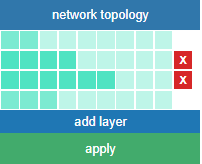
\includegraphics[width=0.25\textwidth]{../Realisierung/bilder/network-topologie} 
\caption{Konfiguration der Netzwerktopologie}\label{abb:network-topologie}
\end{figure}

\begin{figure}[htp]     % h=here, t=top, b=bottom, p=page
\centering
\begin{minipage}[b]{.45\textwidth}
	\centering
	
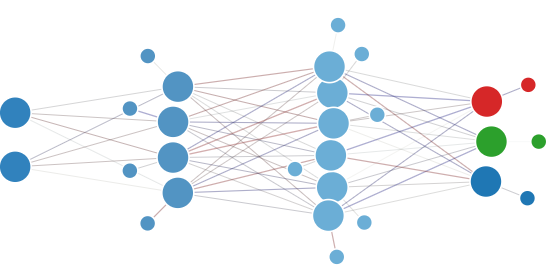
\includegraphics[width=1\textwidth]{../Realisierung/bilder/network-graph}
\captionsetup{format=plain}\caption{Darstellung eines Netzwerkgraphs (untrainiert)}\label{abb:network-graph}
\end{minipage}
\begin{minipage}[b]{.45\textwidth}
\centering
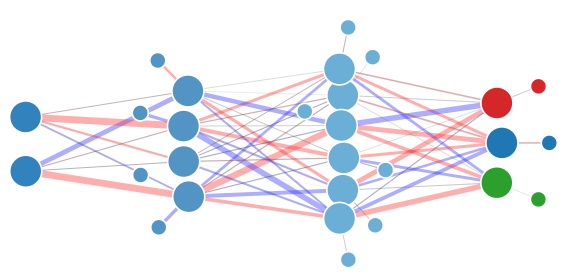
\includegraphics[width=1\textwidth]{../Realisierung/bilder/network-graph-t} 
\captionsetup{format=plain}\caption{Darstellung eines Netzwerkgraphs (trainiert)}\label{abb:network-graph-t}
\end{minipage}
\end{figure}

\subsection{Training}
\subsubsection{Erzeugung der Trainingsdaten}
Zur Erzeugung der Trainingsdaten gibt es eine Fl�che von $300\times300$ px, die als Koordinatensystem gesehen werden kann, auf der rote, gr�ne und blaue Punkte eingetragen werden k�nnen (siehe Abb. \ref{abb:training}). Die Wahl auf diese Farben als Klassen fiel laut Koenecke aufgrund der dadurch gegebenen M�glichkeit, so optimal den RGB-Farbraum darstellen zu k�nnen. Jeder Punkt ist eine Darstellung eines Trainingsdatensatzes, bei dem die x- und die y-Koordinate die Eingabe und die Farbe die erwartete Ausgabe bzw. Klasse darstellt. 

\subsubsection{Trainieren des Netzwerks}
Sind die Trainingsdaten festgelegt, kann �ber den Button \emph{train network} das Training gestartet werden (siehe Abb. \ref{abb:trainingstart}). Der Slider erm�glicht es, das Training zu beschleunigen oder zu verlangsamen. Beim Trainingsprozess ver�ndern sich die Gewichtswerte, dies ist auch bei der Visualisierung des Netzwerkgraphs zu sehen, bei dem sich die Dicken der Linien �ndern (siehe Abb. \ref{abb:network-graph-t}).


\begin{figure}[htp]     % h=here, t=top, b=bottom, p=page
\centering
\begin{minipage}[b]{.45\textwidth}
	\centering
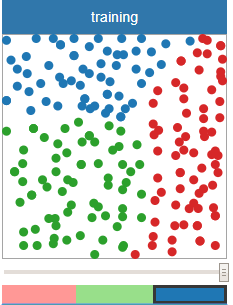
\includegraphics[width=0.4\textwidth]{../Realisierung/bilder/training}
\captionsetup{format=plain}\caption{Erzeugung der Trainingsdaten}\label{abb:training}
\end{minipage}
\begin{minipage}[b]{.45\textwidth}   
\centering
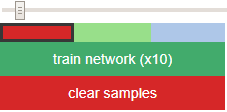
\includegraphics[width=0.6\textwidth]{../Realisierung/bilder/trainingstart} 
\captionsetup{format=plain}\caption{Start des Trainings mit 10-facher Geschwindigkeit}\label{abb:trainingstart}
\end{minipage}
\end{figure}

\subsection{Pr�sentation der Netzwerkergebnisse}
\subsubsection{Vorschau der Ausgabe}
Bei jedem Trainingsschritt wird f�r jeden Punkt des Eingabekoordinatensystems, d.h f�r jede m�gliche Eingabem�glichkeit der x- und der y-Koordinate,\footnote{In diesem Fall gibt es also $300\cdot300=90000$ Eingabem�glichkeiten.} drei Ausgabewerte berechnet, die in der Anwendung die RGB-Werte repr�sentieren. Dadurch ergibt sich die M�glichkeit, die Trainingsergebnisse als Bild zu visualisieren (siehe z.B. Abb. \ref{abb:output-preview1}). Jeder Ausgabewert steht daf�r, wie hoch die Wahrscheinlichkeit ist, dass der Punkt zu einer bestimmten Klasse bzw. Farbe geh�rt. Dadurch kann sich f�r einen Punkt eine Mischfarbe ergeben, wenn sie zwei �hnlich hohe Ausgabewerte hat, meist befindet sie sich in dem Falle nahe der Hyperebene (siehe z.B. Abb. \ref{abb:output-preview2}, bei dem manche Punkte die Mischfarbe gelb-orange oder lila haben). Je mehr Trainingsschritte durchlaufen werden, desto eindeutiger kann jedem Punkt eine Farbe bzw. eine Klasse zugeordnet werden, was sich in der Vorschau dadurch bemerkbar macht, dass die Farben ges�ttigter und die Kanten sch�rfer sind (siehe z.B. Abb. \ref{abb:output-preview3}).

\begin{figure}[htp]     % h=here, t=top, b=bottom, p=page
\centering
\begin{minipage}[b]{.32\textwidth}
	\centering
	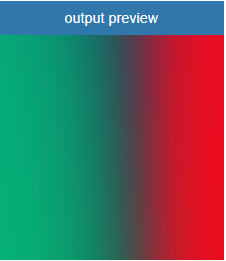
\includegraphics[width=0.9\textwidth]{../Realisierung/bilder/output-preview1} 
	\captionsetup{format=plain}\caption{Vorschau nach einer halben Million Beispieldaten}					\label{abb:output-preview1}
\end{minipage}
\begin{minipage}[b]{.32\textwidth}
	\centering
	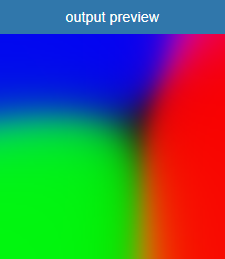
\includegraphics[width=0.9\textwidth]{../Realisierung/bilder/output-preview2} 
	\captionsetup{format=plain}\caption{Vorschau nach einer Million Beispieldaten}	\label{abb:output-preview2}
\end{minipage}
\begin{minipage}[b]{.32\textwidth}
	\centering
	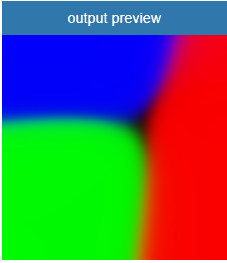
\includegraphics[width=0.9\textwidth]{../Realisierung/bilder/output-preview3} 
	\captionsetup{format=plain}\caption{Vorschau nach drei Millionen Beispieldaten}	\label{abb:output-preview3}
\end{minipage}
\end{figure}

\subsubsection{Netzwerkinfo}
Unter der Vorschau werden dem Anwender bestimmte Informationen des Netzes gezeigt (siehe Abb. \ref{abb:network-info}). Die Information \emph{samples total} gibt die Anzahl der bisher durchgef�hrten Trainingsschritte an, \emph{samples coverage} wie viel Prozent der Trainingspunkte durch das KNN korrekt klassifiziert wurden und \emph{mean weight change} wie hoch die durchschnittliche Gewichts�nderung ist. 

\begin{figure}[htp]     % h=here, t=top, b=bottom, p=page
\centering
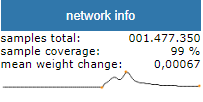
\includegraphics[width=0.3\textwidth]{../Realisierung/bilder/network-info} 
\caption{Netzwerkinfo w�hrend des Trainings}\label{abb:network-info}
\end{figure}

\chapter{Eigene Implementierungen}
\section{Implementierung des KNN in Javascript}
\subsection{Wahl der passenden Javascript Bibliothek f�r das KNN}
Bei der Recherche stellte sich heraus, dass es bereits einige Javascript Bibliotheken gibt, mit denen KNN erstellt und lokal im Browser trainiert werden k�nnen. In die engere Auswahl fielen \emph{brain.js}, \emph{Mind}, \emph{Neataptic} und \emph{Synaptic}. F�r jede Bibliothek wurde ein Testprogramm geschrieben, um sie besser miteinander vergleichen zu k�nnen, wobei jedes Programm dieselben Trainingsbedingungen hat. Grob zusammengefasst, besteht jeder Trainingsdatensatz aus zwei Punkten, denen eine Klasse zugeordnet wurde. F�r das Training wird bei jedem eine bestimmte Topologie festgelegt und eine bestimmte Anzahl an Iterationen durchgef�hrt. Am Ende des Trainings sollte angegeben werden, wie die berechneten Ausgabewerte der Punkte aussehen und wie lange das Training gedauert hat. Die Testprogramme befinden sich in der CD im Ordner \emph{NNBibTests}.\footnote{Ebenfalls wurde aus Interesse zum Vergleich f�r die Bibliothek \emph{ConvNetJS} ein Testprogramm geschrieben, die bei der Berechnung deutlich am pr�zisesten und schnellsten war, allerdings werden dort keine MLP zur Berechnung genutzt, sondern sogenannte \emph{Convolutional Neural Networks}, eine besondere Form von Feedforward Netzen.} 

Folgende Punkte waren wichtig f�r die Wahl der Bibliothek gewesen: 
\begin{itemize}
\item die M�glichkeit, ein MLP erstellen zu k�nnen
\item die Handhabung mit der Bibliothek (z.B. wie aufw�ndig ist es, den Code zur Erstellung des MLP oder des Trainings zu schreiben)
\item die Geschwindigkeit der Berechnung 
\item die Effektivit�t des Trainings
\item die Dokumentation der Bibliothek
\item die �bersichtlichkeit und Struktur des Codes der Bibliothek
\item zu einem geringen Teil die Aktivit�t an der Bibliothek, also wie oft die Bibliothek aktualisiert wurde und wann die letzte Aktualisierung stattfand
\end{itemize}

In der Handhabung konnten brain.js und Mind ganz gut punkten, so ist es schon mit wenigen Zeilen Code m�glich, ein KNN zu erstellen. Allerdings sind die Konfigurationsm�glichkeiten des KNN mit den beiden Bibliotheken eher beschr�nkt und beide bieten eine eher d�rftige Dokumentation. Bei Neataptic handelt es sich um eine Bibliothek, die f�r bestimmte Teile des Codes die Synaptic Bibliothek verwendet hat. Von allen betrachteten Bibliotheken bietet sie auch mit einem Wiki aus 30 Seiten die beste Dokumentation und bietet gegen�ber Synaptic Extras wie die Visualisierung der Topologie des KNN, mehr implementierte Aktivierungsfunktion etc. Allerdings handelt es sich um Extras, die f�r den eigentlichen Zweck des Programms nicht notwendig sind. Schlussendlich fiel die Wahl auf Synaptic, deren ausschlaggebendster Vorteil die M�glichkeit ist, das Training �ber Web Worker durchf�hren lassen zu k�nnen. Was Web Worker sind und weshalb sie einen Vorteil f�r die Anwendung bringen, soll im Kapitel \ref{ch:multiWW} erl�utert werden.

\subsection{Performancevorteile durch Nutzung von Web Workern}\label{ch:multiWW}
\subsubsection{Problem der Synchronit�t und des Single-Threadings}
Allgemein kann Javascript als eine Programmiersprache betrachtet werden, die normalerweise \emph{synchron} und \emph{single-threaded} l�uft. Single-threaded bedeutet, dass zur gleichen Zeit nur ein Prozess stattfinden kann \citep{brij}. Von synchroner Programmierung spricht man, wenn der Start von einem Prozess das ganze Programm solange zum Stoppen bringt, bis der Prozess zu Ende ausgef�hrt wurde. Das bedeutet also, dass bei Javascript die Prozesse sequenziell bzw. nacheinander abgearbeitet werden. 

Bezogen auf die Anwendung f�r die Bachelorarbeit stellt diese Eigenschaft ein ung�nstiges Problem da. F�r das Training werden komplexe Berechnungen durchgef�hrt, besonders bei der Backpropagation finden viele Berechnungsschritte statt. Das Training des MLP mit der Methode \emph{train()} der Synaptic Bibliothek f�hrte dazu, dass die Bedienung der GUI w�hrend des Trainings sehr tr�ge wirkte. Bis auf Interaktionen vom Anwender wie ein Mausklick auf einen Button reagiert wurde, vergingen teilweise mehrere Sekunden. 

\subsubsection{Multithreading mithilfe von Web Workern}
Es musste eine passende Technik gefunden werden, die Nebenl�ufigkeit bzw. Multithreading in Javascript zu erm�glichen, d.h. mehrere Prozesse gleichzeitig ausf�hren lassen zu k�nnen. Denn um dem Anwender eine reaktionsschnelle GUI bieten zu k�nnen, m�ssen die Berechnungen f�r das Trainings nebenl�ufig laufen. Es gibt verschiedene Wege die Nebenl�ufigkeit in Javascript nachzuahmen, wie die Verwendung von \emph{setTimeout()}, \emph{setInterval()}, \emph{XMLHttpRequest} oder  Ereignis-Handlern \citep{bidelman}. Allerdings findet bei diesen Techniken alles immer noch im selben Hauptthread\footnote{Bei einem Thread handelt es sich um eine Aktivit�t innerhalb eines Prozesses. Jeder Prozess besteht aus mindestens einem Thread, dem Hauptthread. Neben dem Hauptthread k�nnen im Prozess noch weitere Threads ausgef�hrt werden \citep{wolf}.} im Browser statt, so wechseln sich lediglich die Prozesse der Skriptausf�hrungen mit den Aktivit�ten der GUI ab. Web Worker sind eine Javascript API\footnote{Schnittstelle zur Anwendungsprogrammierung (engl.: application programming interface} f�r HTML5, mit der tats�chlich im Hintergrund Skripte �ber mehrere Threads ausgef�hrt werden k�nnen. 

Zum Testen der Geschwindigkeit gibt es f�r die Synaptic Bibliothek im Ordner \emph{synaptic-withoutWW} ein Testprogramm, welches das Training normal ohne einen Web Worker ausf�hrt und im Ordner \emph{synaptic-withWW} ein Testprogramm, welches das Training mit einem Web Worker ausf�hrt. Auf dem getesteten Rechner fiel beim Vergleichen der Zeiten auf, dass sogar mit dem Web Worker eine bessere Zeit erzielt wurde (ca. 750 ms gegen�ber ca. 1000 ms ohne Web Worker). Bei der Implementierung des MLP mit Synaptic ist auch deutlich aufgefallen, dass durch die Nutzung eines Web Workers die GUI w�hrend des Trainings deutlich schneller auf die Interaktionen des Anwenders reagiert hat. 

\subsection{Trainieren eines MLP mit Synaptic}
In der Javascript Datei \emph{neural-network.js} ist der Codeteil zu finden, in dem das MLP erstellt und trainiert wird. Es soll hier in dieser Arbeit nicht der ganze Code erl�utert werden, sondern nur kurz auf den interessanten Codeteil, der f�r das Training eingegangen werden (siehe Listing \ref{lis:jsTraining}). 
Bei \emph{trainAsync()} handelt es sich sich um eine Methode f�r das Perzeptron, das Training in einem Webworker stattfinden lassen zu k�nnen. Der Parameter \emph{rate} legt die Lernrate und \emph{iterations} legt die maximale Anzahl an Iterationen fest, diese wurden vom Anwender zuvor in der GUI festgelegt. Der \emph{error} gibt den Wert an, der unterschritten werden muss, bis das Training beendet werden kann. Durch \emph{cost} wird die Fehlerfunktion festgelegt, in diesem Fall wird der MSE genommen, der im Kapitel \ref{ch:bb-regel} erw�hnt wurde. Mit \emph{myTrainer.trainAsync()} wird ein Promise-Objekt \emph{promiseTrain} erstellt, der bei erfolgreicher Operation mit \emph{promiseTrain.then()}, die Trainingsergebnisse an die Funktion \emph{updateAndSendMessageForApp} �bergibt.\footnote{Das Promise-Objekt wird dazu verwendet, um asynchrone Berechnungen durchf�hren zu k�nnen. Genaueres zu der Technologie kann auf der Seite \url{https://developer.mozilla.org/de/docs/Web/JavaScript/Reference/Global_Objects/Promise} nachgelesen werden.} Dieser f�hrt wiederum die Operationen durchf�hrt, damit die Ergebnisse sp�ter in der GUI visualisiert werden k�nnen. 

\begin{lstlisting}[language=JavaScript,caption={Codeausschnitt des Trainings eines MLP mit Synaptic},label=lis:jsTraining,captionpos=b]
var promiseTrain = myTrainer.trainAsync(trainingSet, {
	rate: messageForApp.nnConfigInfo.learningRate,
	iterations: iterations,
	error: 0.000000000000000000000000000000000000000000000000000000000001,
	cost: Trainer.cost.CROSS_ENTROPY
});
promiseTrain.then(function (results) {
	returnObj = {
		"myPerceptron": myPerceptron,
		"samplesTrained": (samplesTrained += iterations),
		"trainingsSetLength": trainingSet.length
	}
	getUpdatedMessageForApp(JSON.stringify(returnObj));
});
\end{lstlisting}

\subsubsection{Aufbau eines Perzeptrons in Synaptic}
Vereinfacht sieht der Code eines Perzeptrons in Synaptic als JSON wie in Listing \ref{lis:jsonPerc} aus. Die Attribute \emph{\glqq input\grqq } und\emph{\glqq output\grqq} bekommen beide jeweils als Wert ein Layer-Objekt (siehe Listing \ref{lis:jsonLayer}) zugewiesen, sie stellen die Eingabeschicht und die Ausgabeschicht des MLP dar. Das Attribut \emph{\glqq hidden\grqq} bekommt als Wert ein Array zugewiesen, welches aus mehreren Layer-Objekten besteht, welches die versteckten Schichten darstellen.
\begin{lstlisting}[language=json, caption={JSON eines Perzeptron-Objekts in Synaptic},label=lis:jsonPerc,captionpos=b]
{"layers" = {
	"hidden":[...a\dots a...],			
	"input":{...a\dots a...},
	"ouput":{...a\dots a...}
}}
\end{lstlisting}

Das Listing der JSON vom Layer-Objekt ist stark vereinfacht, indem nur die Attribute und Werte angezeigt werden, die f�r die Visualisierung des MLP in der GUI von Bedeutung sind.  

\begin{lstlisting}[language=json, caption={JSON eines Layer-Objekts},label=lis:jsonLayer,captionpos=b]
{"Layer":{		
	"list":[
		"Neuron":{
			"ID": 5,
			"activation": 0,
			"bias": 0.46,
			"connections":{
				"projected":{
					"Connection":{
						"from":{
							"ID": 5,
							...a\dots a...
						},
						"to":{
							"ID": 7,
							...a\dots a...
						},
						"weight": 6.553,
						...a\dots a...
					},
					...a\dots a...
				},
				...a\dots a...
			},
			...a\dots a...
		},
		...a\dots a...
	],
	"size": 5,
	...a\dots a...
}}
\end{lstlisting}

\subsection{Schnittstelle zwischen der Netzwerkbibliothek und der GUI}
Dem Vorteil von Web Workern, dass rechenintensive Skripte nicht mehr im Hauptthread ausgef�hrt werden m�ssen, stehen einige Nachteile gegen�ber. Im Bezug auf die Anwendung f�r die Bachelorarbeit sind die wichtigsten Nachteile, dass Web Worker nicht in der Lage sind, das DOM\footnote{DOM: Document Object Model; Programmierschnittstelle f�r HTML und XML Dokumente} zu �ndern und dass sie nicht auf globale Variablen und Funktionen zugreifen k�nnen \citep{buckler}. F�r die Anwendung bedeutet dies, dass w�hrend des Trainingsvorgangs, indem die intensiven Berechnungen stattfinden, die GUI nicht ver�ndert werden kann. 

In seiner Bachelorthesis hat Koenecke die Vermutung aufgestellt, dass eine Implementierung des KNN in Javascript wohl keine Schnittstelle zur Kommunikation zwischen der Netzwerkbibliothek und der GUI erfordert h�tte \citep[S.42]{koenecke}. Im Grunde genommen hat er damit Recht, dies setzt jedoch voraus, dass die Berechnungen des Trainings im Hauptthread stattfinden, um w�hrenddessen gleichzeitig die GUI ver�ndern zu k�nnen. Wie bereits vorher erl�utert, w�rde dies aber zu sehr die Performance verschlechtern und daher ist die Verwendung von Web Workern zu bevorzugen. Um einen Austausch der Trainingsergebnisse mit den Interaktionen der GUI zu erm�glichen, hat es sich also weiterhin angeboten die Schnittstelle zur Kommunikation beizubehalten. Zudem gew�hrleistet eine Trennung der Netzwerkbibliothek von der GUI eine bessere �bersichtlichkeit vom Code der Anwendung. Wie auch in Koeneckes Anwendung stellt die Javascript-Datei \emph{app.js} die Schnittstelle dar, mit dem Unterschied, dass in dieser Anwendung kein Server und daher keine emulierten Websockets mehr ben�tigt werden. 

\subsubsection{Aufbau eines message-Objektes f�r die GUI} 
In der Schnittstelle wird zur Erstellung des MLP mit der Methode \emph{newNetwork()} und zum Updaten des MLP mit der Methode \emph{updateNetwork()} in der GUI ein message-Objekt mit einer bestimmten Struktur ben�tigt (siehe Listing \ref{lis:jsonMessage}). Sie entspricht zum gr��ten Teil dem message-Objekt von Koenecke, aufgrund der Erweiterungen in der Anwendung wurde das message-Objekt etwas erweitert. In der \emph{neural-network.js} wurden zur Erstellung der message-Objekte in diesem Format die Funktionen \emph{getMessageForApp()} und \emph{getUpdatedMessageForApp()} geschrieben.

\begin{lstlisting}[language=json, caption={JSON eines Perzeptron-Objekts in Synaptic},label=lis:jsonMessage,captionpos=b]
{"message" = {
	"bMaxIterationsReached": false,
	"nnConfigInfo": {
		"activationFunction": "relu",
		"learningRate": 0.01,
		"maxIterations": 100000
	},
	"id": 1,
	"graph":{
		"layers": [
			{
				"numberOfNeurons": 3,
				"weights":{
					"data":[
						{0.54, 0.945, 0.435},
						...a\dots a...
					]
				}
			},
			...a\dots a...
		],
		"sampleCoverage": 0,
		"samplesTrained":0,
		"weightChange":0
	}	
	"output":{
		"data": [
			[253, 0, 0],
			...a\dots a...
		]
	}
}}
\end{lstlisting}

\section{Erweiterungen an der GUI}
\subsection{Konfiguration der Aktivierungsfunktion und der Lernrate}
Die Konfiguration des MLP wurde erweitert, dass nicht nur die Topologie, sondern auch die Aktivierungsfunktion und die Lernrate festgelegt werden kann (siehe Abb. \ref{abb:network-config}). So kann der Anwender besser verstehen, inwiefern diese beiden Parameter das Training des Netzwerks beeinflussen k�nnen. Beide Parameter m�ssen beim Start festgelegt werden und k�nnen nicht w�hrend des Trainings ver�ndert werden. 
\begin{figure}[htp]     % h=here, t=top, b=bottom, p=page
\centering
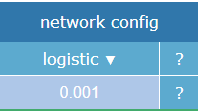
\includegraphics[width=0.25\textwidth]{../Realisierung/bilderErw/network-config} 
\caption{Die Aktivierungsfunktion und die Lernrate k�nnen nun ver�ndert werden}\label{abb:network-config}
\end{figure}
\subsection{Erweiterungen beim Training}
Das Feld zum Setzen der Trainingspunkte wurde um zwei Koordinatenachsen erweitert, wodurch die Trainingspunkte besser positioniert werden k�nnen (siehe Abb. \ref{abb:training-sCreate}). Zudem kann der Anwender durch die Achsen m�glicherweise besser verstehen, dass die x- und y-Koordinate als Eingabeparameter f�r jeden Trainingsdatensatz zu sehen sind. Ist ein Trainingspunkt ausgew�hlt, so hat man die M�glichkeit durch die beiden Eingabefelder \emph{x} und \emph{y} genaue Werte f�r die Koordinaten zu setzen oder den Trainingspunkt zu l�schen. Die Liste darunter bietet eine weitere �bersicht, um zu veranschaulichen, welche Trainingspunkte beim Start des Trainings �bergeben werden.
\begin{figure}[htp]     % h=here, t=top, b=bottom, p=page
\centering
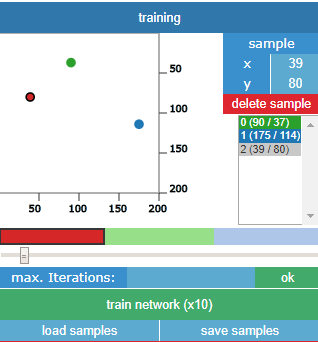
\includegraphics[width=0.45\textwidth]{../Realisierung/bilderErw/trainingGes} 
\caption{Das neue Trainingselement}\label{abb:training-sCreate}
\end{figure}
Beim Eingabefeld \emph{max. Iterations} kann festgelegt werden, nach wie vielen Trainingsiterationen das Training gestoppt werden kann (siehe Abb. \ref{abb:training-sCreate}). Es ist m�glich, nach dem Stoppen des Trainings den Wert zu erh�hen und das Training fortzuf�hren. Auch w�hrend des Trainings kann der Wert ver�ndert werden. Gedacht ist die Erweiterung als eine M�glichkeit, besser die Effektivit�t des Trainings vergleichen zu k�nnen, wenn beispielsweise eine andere Aktivierungsfunktion gew�hlt wurde. Durch einen Klick auf den Button \emph{save samples} k�nnen die Trainingsdaten lokal im Webbrowser gespeichert werden, sodass man die Anwendung auch schlie�en kann und mit \emph{load samples} die Trainingsdaten zu einem sp�teren Zeitpunkt wieder aufrufen kann. 

\subsection{Aufgaben ausw�hlen}
Der Anwender hat nun zus�tzlich die M�glichkeit anhand gestellter �bungen spielerisch zu erlernen, wie das KNN f�r bestimmte Probleme konfiguriert werden sollte (siehe Abb. \ref{abb:exercise}). Zu jeder �bung gibt es eine \emph{tasklist} mit mehreren \emph{tasks}. Wurde eine Task gel�st, so �ndert sich die Textfarbe der Task (siehe Abb. \ref{abb:tasksolved}). Momentan sind in der Anwendung lediglich \textcolor{red}{drei} �bungen vorhanden, die noch eher einfach gehalten sind. 

\begin{figure}[htp]     % h=here, t=top, b=bottom, p=page
\centering
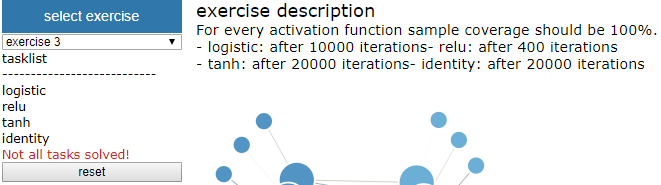
\includegraphics[width=1\textwidth]{../Realisierung/bilderErw/exercise} 
\caption{Screenshot von einer �bung}\label{abb:exercise}
\end{figure}

\begin{figure}[htp]     % h=here, t=top, b=bottom, p=page
\centering
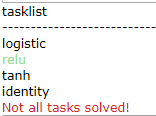
\includegraphics{../Realisierung/bilderErw/tasksolved} 
\caption{Der Task f�r die ReLu Aktivierungsfunktion wurde gel�st.}\label{abb:tasksolved}
\end{figure}

\chapter{Konfiguration eines KNN passend zur Problemstellung}


%______________________________________


\newpage
\chapter*{Abk�rzungsverzeichnis}
\begin{acronym}{}
\acro{MLP}[MLP]{mehrlagige Perzeptron}
\acro{KI}[KI]{K�nstliche Intelligenz}
\acro{KNN}[KNN]{k�nstliche neuronale Netze}
\acro{GUI}[GUI]{Grafical User Interface}
\end{acronym}

%--------------------- VERZEICHNISSE ----------------

\listoffigures % Abbildungsverzeichnis erzeugen
\listoftables % Tabellenverzeichnis erzeugen

%--------------------- LITERATURLISTE ---------------
% Die Eintr�ge sollen alphabetisch sortiert sein.

\begin{thebibliography}{}

\bibitem[Bidelman(2010)]{bidelman} 
Bidelman, Eric: 
\emph{Web Worker-Grundlagen}, 
\url{https://www.html5rocks.com/de/tutorials/workers/basics/}, 26.07.2010, letzter Zugriff: 29. 08. 2017

\bibitem[Brij(2015)]{brij} 
Brij: 
\emph{Concurrency vs Multi-threading vs Asynchronous Programming : Explained}, 
\url{https://codewala.net/2015/07/29/concurrency-vs-multi-threading-vs-asynchronous-programming-explained/}, 29.07.2015, letzter Zugriff: 29. 08. 2017

\bibitem[Buckler(2013)]{buckler} 
Buckler, Craig: 
\emph{Implementing JavaScript Threading with Web Workers}, 
\url{https://www.safaribooksonline.com/blog/2013/10/24/implementing-javascript-threading-with-web-workers/}, 24.10.2013, letzter Zugriff: 29. 08. 2017

\bibitem[Corves(2005)]{corves} 
Corves, Anna: 
\emph{Nervenzellen im Gespr�ch}, 
\url{https://www.dasgehirn.info/grundlagen/kommunikation-der-zellen/nervenzellen-im-gespraech?gclid=COiWg7TdzNQCFU4W0wodK74IwA}, 2012, letzter Zugriff: 1. 07. 2017

\bibitem[Ertel(2016)]{ertel}
Ertel, Wolfgang: 
\emph{Grundkurs K�nstliche Intelligenz : Eine praxisorientierte Einf�hrung}, 4. Aufl., Berlin Heidelberg New York: Springer-Verlag, 2016

\bibitem[Hebb(1949)]{hebb}
Hebb, Donald Olding: 
\emph{The Organization Of Behavior: A Neuropsychological Theory}, Psychology Press edition 2002, 1949

\bibitem[Hillmann()]{hillmann} 
Hillmann, Leonard: 
\emph{Intelligentes Leben}, 
\url{http://www.tagesspiegel.de/themen/gehirn-und-nerven/gesund-leben-intelligentes-leben/13410564.html}, Ver�ffentlichkeitsdatum unbekannt, letzter Zugriff: 01.07.2017

\bibitem[Hoffmann(1993)]{hoffmann} 
Hoffmann, Norbert
\emph{Kleines Handbuch Neuronale Netze : Anwendungsorientiertes Wissen zum Lernen und Nachschlagen}, Berlin Heidelberg New York: Springer-Verlag, 1993

\bibitem[Koenecke(2016)]{koenecke}
Koenecke, Finn Ole: 
\emph{Realisierung eines interaktiven k�nstlichen neuronalen Netzwerks}, 2016

\bibitem[Kramer(2009)]{kramer}
Kramer, Oliver: 
\emph{Computational Intelligence : Eine Einf�hrung}, 1. Aufl., Berlin Heidelberg New York: Springer-Verlag, 2009.

\bibitem[Manhart (2017)]{manhart}
Manhart, Klaus: 
\emph{Was Sie �ber Maschinelles Lernen wissen m�ssen},
\url{https://www.computerwoche.de/a/was-sie-ueber-maschinelles-lernen-wissen-muessen,3329560}, 04.05.2017, letzter Zugriff: 02.07.2017

\bibitem[Minsky \& Papert(1969)]{minsky_papert}
Minsky, Marvin; Papert, Seymour:
\emph{Perceptrons: An Introduction to Computational Geometry}, 2nd edition with corrections, first edition 1969 , The MIT Press, Cambridge MA, 1972.

\bibitem[Rey \& Wender(1982)]{rey_wender}
Rey, G�nter Daniel ; Wender, Karl F.: 
\emph{Neuronale Netze : eine Einf�hrung in die Grundlagen, Anwendungen und Datenauswertung}, 2. vollst. �berarb. und erw. Aufl., Bern: Huber, 2011.

\bibitem[Riley(2017)]{riley}
Riley, Tonya: 
\emph{Artificial intelligence goes deep to beat humans at poker},
\url{http://www.sciencemag.org/news/2017/03/artificial-intelligence-goes-deep-beat-humans-poker}, 03.03.2017, letzter Zugriff: 07.07.2017

\bibitem[Rimscha(2014)]{rimscha}
Rimscha, Markus: 
\emph{Algorithmen kompakt und verst�ndlich : L�sungsstrategien am Computer}, 3. Aufl., Berlin Heidelberg New York: Springer-Verlag, 2014.

\bibitem[Russell \& Norvig(2010)]{russell-norvig}
Russell, Stuart ; Norvig, Peter:
\emph{Artificial Intelligence : A Modern Approach}, 3. Aufl(2010), London: Prentice Hall, 2010.

\bibitem[Scherer(1997)]{scherer}
Scherer, Andreas: Neuronale Netze : Grundlagen und Anwendungen. Berlin Heidelberg New York: Springer-Verlag, 1997.

\bibitem[SethBling(2015)]{sethBling}
SethBling: 
\emph{MarI/O - Machine Learning for Video Games},
\url{https://www.youtube.com/watch?v=qv6UVOQ0F44}, 13.06.2017, letzter Zugriff: 07.07.2017

\bibitem[Turing(1950)]{turing}
Turing, Alan M.: 
\emph{Computing Machinery and Intelligence}, Mind, 59, 1950.

\bibitem[Wolf(2009)]{wolf}
Wolf, J�rgen: 
\emph{C von A bis Z : das umfassende Handbuch},
\url{http://openbook.rheinwerk-verlag.de/c_von_a_bis_z/026_c_paralleles_rechnen_003.htm}  Bonn: Rheinwerk Verlag GmbH, 2009, letzter Zugriff: 29.08.2017

\bibitem[Wunderlich-Pfeiffer(2017)]{wunderlich}
Wunderlich-Pfeiffer, Frank : 
\emph{Alpha Go geht in Rente},
\url{https://www.golem.de/news/kuenstliche-intelligenz-alpha-go-geht-in-rente-1705-128059.html}, 29.05.2017, letzter Zugriff: 04.07.2017

\bibitem[Zell(1994)]{zell}
Zell, Andreas: 
\emph{Simulation neuronaler Netze}, 4.Auflage(2003) Deutschland: Oldenbourg Wissenschaftsverlag GmbH, 1994.

\end{thebibliography}
 
\end{document} 

%chapter Verwandte Arbeiten



\newpage
\chapter*{Abk�rzungsverzeichnis}
\begin{acronym}{}
\acro{MLP}[MLP]{mehrlagige Perzeptron}
\acro{KI}[KI]{K�nstliche Intelligenz}
\acro{KNN}[KNN]{k�nstliche neuronale Netze}
\acro{GUI}[GUI]{Grafical User Interface}
\end{acronym}

%--------------------- VERZEICHNISSE ----------------

\listoffigures % Abbildungsverzeichnis erzeugen
\listoftables % Tabellenverzeichnis erzeugen

%--------------------- LITERATURLISTE ---------------
% Die Eintr�ge sollen alphabetisch sortiert sein.

\begin{thebibliography}{}

\bibitem[Bidelman(2010)]{bidelman} 
Bidelman, Eric: 
\emph{Web Worker-Grundlagen}, 
\url{https://www.html5rocks.com/de/tutorials/workers/basics/}, 26.07.2010, letzter Zugriff: 29. 08. 2017

\bibitem[Brij(2015)]{brij} 
Brij: 
\emph{Concurrency vs Multi-threading vs Asynchronous Programming : Explained}, 
\url{https://codewala.net/2015/07/29/concurrency-vs-multi-threading-vs-asynchronous-programming-explained/}, 29.07.2015, letzter Zugriff: 29. 08. 2017

\bibitem[Buckler(2013)]{buckler} 
Buckler, Craig: 
\emph{Implementing JavaScript Threading with Web Workers}, 
\url{https://www.safaribooksonline.com/blog/2013/10/24/implementing-javascript-threading-with-web-workers/}, 24.10.2013, letzter Zugriff: 29. 08. 2017

\bibitem[Corves(2005)]{corves} 
Corves, Anna: 
\emph{Nervenzellen im Gespr�ch}, 
\url{https://www.dasgehirn.info/grundlagen/kommunikation-der-zellen/nervenzellen-im-gespraech?gclid=COiWg7TdzNQCFU4W0wodK74IwA}, 2012, letzter Zugriff: 1. 07. 2017

\bibitem[Ertel(2016)]{ertel}
Ertel, Wolfgang: 
\emph{Grundkurs K�nstliche Intelligenz : Eine praxisorientierte Einf�hrung}, 4. Aufl., Berlin Heidelberg New York: Springer-Verlag, 2016

\bibitem[Hebb(1949)]{hebb}
Hebb, Donald Olding: 
\emph{The Organization Of Behavior: A Neuropsychological Theory}, Psychology Press edition 2002, 1949

\bibitem[Hillmann()]{hillmann} 
Hillmann, Leonard: 
\emph{Intelligentes Leben}, 
\url{http://www.tagesspiegel.de/themen/gehirn-und-nerven/gesund-leben-intelligentes-leben/13410564.html}, Ver�ffentlichkeitsdatum unbekannt, letzter Zugriff: 01.07.2017

\bibitem[Hoffmann(1993)]{hoffmann} 
Hoffmann, Norbert
\emph{Kleines Handbuch Neuronale Netze : Anwendungsorientiertes Wissen zum Lernen und Nachschlagen}, Berlin Heidelberg New York: Springer-Verlag, 1993

\bibitem[Koenecke(2016)]{koenecke}
Koenecke, Finn Ole: 
\emph{Realisierung eines interaktiven k�nstlichen neuronalen Netzwerks}, 2016

\bibitem[Kramer(2009)]{kramer}
Kramer, Oliver: 
\emph{Computational Intelligence : Eine Einf�hrung}, 1. Aufl., Berlin Heidelberg New York: Springer-Verlag, 2009.

\bibitem[Manhart (2017)]{manhart}
Manhart, Klaus: 
\emph{Was Sie �ber Maschinelles Lernen wissen m�ssen},
\url{https://www.computerwoche.de/a/was-sie-ueber-maschinelles-lernen-wissen-muessen,3329560}, 04.05.2017, letzter Zugriff: 02.07.2017

\bibitem[Minsky \& Papert(1969)]{minsky_papert}
Minsky, Marvin; Papert, Seymour:
\emph{Perceptrons: An Introduction to Computational Geometry}, 2nd edition with corrections, first edition 1969 , The MIT Press, Cambridge MA, 1972.

\bibitem[Rey \& Wender(1982)]{rey_wender}
Rey, G�nter Daniel ; Wender, Karl F.: 
\emph{Neuronale Netze : eine Einf�hrung in die Grundlagen, Anwendungen und Datenauswertung}, 2. vollst. �berarb. und erw. Aufl., Bern: Huber, 2011.

\bibitem[Riley(2017)]{riley}
Riley, Tonya: 
\emph{Artificial intelligence goes deep to beat humans at poker},
\url{http://www.sciencemag.org/news/2017/03/artificial-intelligence-goes-deep-beat-humans-poker}, 03.03.2017, letzter Zugriff: 07.07.2017

\bibitem[Rimscha(2014)]{rimscha}
Rimscha, Markus: 
\emph{Algorithmen kompakt und verst�ndlich : L�sungsstrategien am Computer}, 3. Aufl., Berlin Heidelberg New York: Springer-Verlag, 2014.

\bibitem[Russell \& Norvig(2010)]{russell-norvig}
Russell, Stuart ; Norvig, Peter:
\emph{Artificial Intelligence : A Modern Approach}, 3. Aufl(2010), London: Prentice Hall, 2010.

\bibitem[Scherer(1997)]{scherer}
Scherer, Andreas: Neuronale Netze : Grundlagen und Anwendungen. Berlin Heidelberg New York: Springer-Verlag, 1997.

\bibitem[SethBling(2015)]{sethBling}
SethBling: 
\emph{MarI/O - Machine Learning for Video Games},
\url{https://www.youtube.com/watch?v=qv6UVOQ0F44}, 13.06.2017, letzter Zugriff: 07.07.2017

\bibitem[Turing(1950)]{turing}
Turing, Alan M.: 
\emph{Computing Machinery and Intelligence}, Mind, 59, 1950.

\bibitem[Wolf(2009)]{wolf}
Wolf, J�rgen: 
\emph{C von A bis Z : das umfassende Handbuch},
\url{http://openbook.rheinwerk-verlag.de/c_von_a_bis_z/026_c_paralleles_rechnen_003.htm}  Bonn: Rheinwerk Verlag GmbH, 2009, letzter Zugriff: 29.08.2017

\bibitem[Wunderlich-Pfeiffer(2017)]{wunderlich}
Wunderlich-Pfeiffer, Frank : 
\emph{Alpha Go geht in Rente},
\url{https://www.golem.de/news/kuenstliche-intelligenz-alpha-go-geht-in-rente-1705-128059.html}, 29.05.2017, letzter Zugriff: 04.07.2017

\bibitem[Zell(1994)]{zell}
Zell, Andreas: 
\emph{Simulation neuronaler Netze}, 4.Auflage(2003) Deutschland: Oldenbourg Wissenschaftsverlag GmbH, 1994.

\end{thebibliography}
 

%--------------------- EIGENST�NDIGKEITSERKL�RUNG ---------------
\clearpage\thispagestyle{empty}
\eigen  % im header definiert
%--------------------------------------- ENDE ------------------------------------
\end{document}
%%%%%%%%%%%%%%%%%%%%%%%%%%%%%%%%%%%%


















